\section{Signal Shapes and Efficiencies}
\label{signalinputs}
 For all plots showing fits to the signal distributions, the red histograms show the distribution of events which pass both the fiducial selection at generator level and pass the full reconstruction level selection, including the selection on $\pt(\mathrm{H})$. The red curve shows a fit to this distrubtion using a double-sided crystal ball function, and the resulting $\sigma$ of the fit is also shown on the plot. The blue histograms show events which pass the full reconstruction level selection, and pass the fiducial selection at generator level within a different $\pt(\mathrm{H})$ bin. The blue curves show a fit to this distrubtion using the same function as the red curve with a different normalization. The black histograms show the distribution of events which pass the full reconstruction level selection but do not pass the fiducial selection at generator level, and the black curve shows a fit to this distribution using the same function as the red curve but with a different normalization. The yellow histogram shows events which pass the full reconstruction level selection but where one of the four selected leptons does not originate from the Higgs boson. The yellow curve shows a fit to this distribution using a Landau function.
 
\subsection[Differential bins - Higgs boson transverse momentum]{Fits in different bins of $\pt(\mathrm{H})$ }

\begin{figure}[htb]
  \begin{center}
    \subfigure[$0.0 < \pt(\mathrm{H}) < 15.0 $]{
      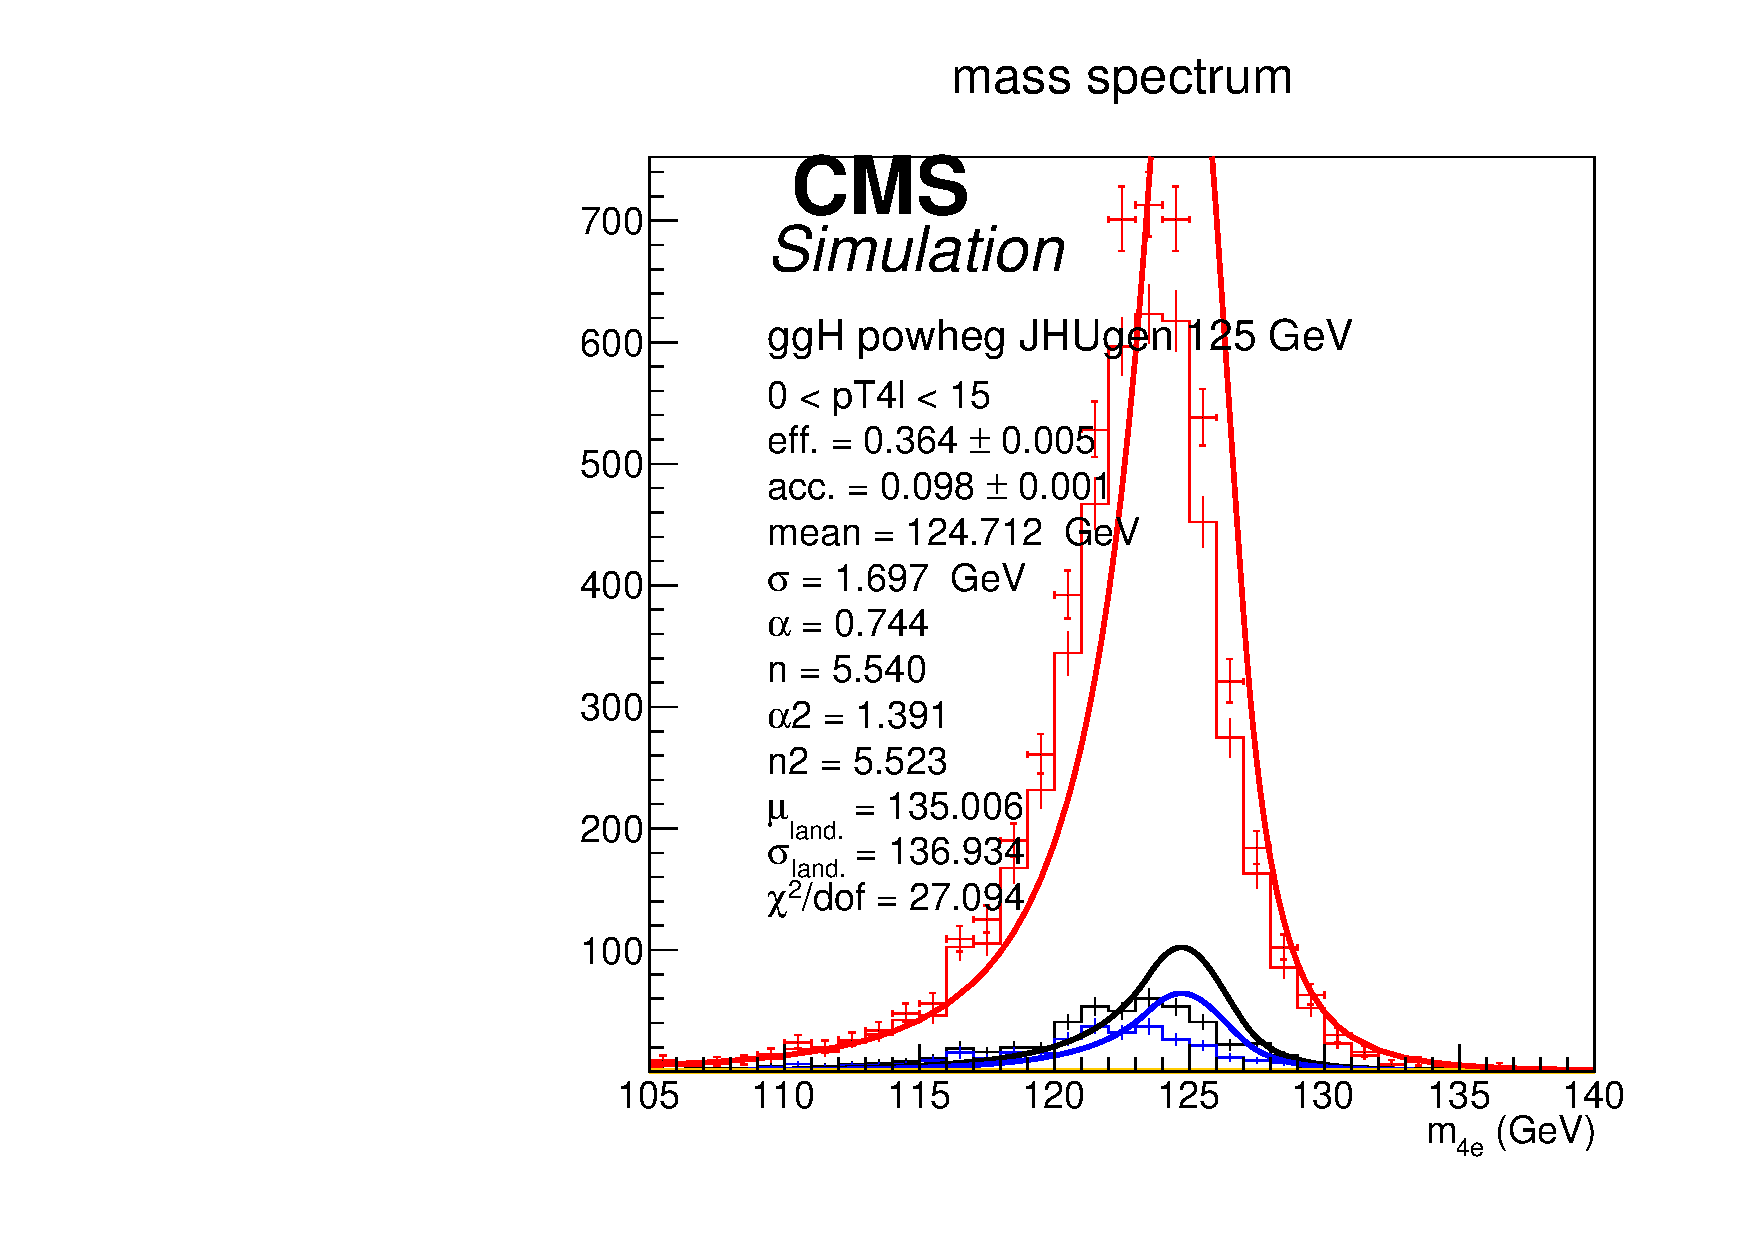
\includegraphics[width=0.3\textwidth,angle=0]{Figures/Appendix//ggH_powheg_JHUgen_125_4e_pT4l_genbin0_recobin0_effs_genWeight*pileupWeight*dataMCWeight.pdf}
      \label{fig:sigfits-pT4l-ggH-powheg15-JHUgen-125-maintext:a}
    }
    \subfigure[$15.0 < \pt(\mathrm{H}) < 30.0$]{
      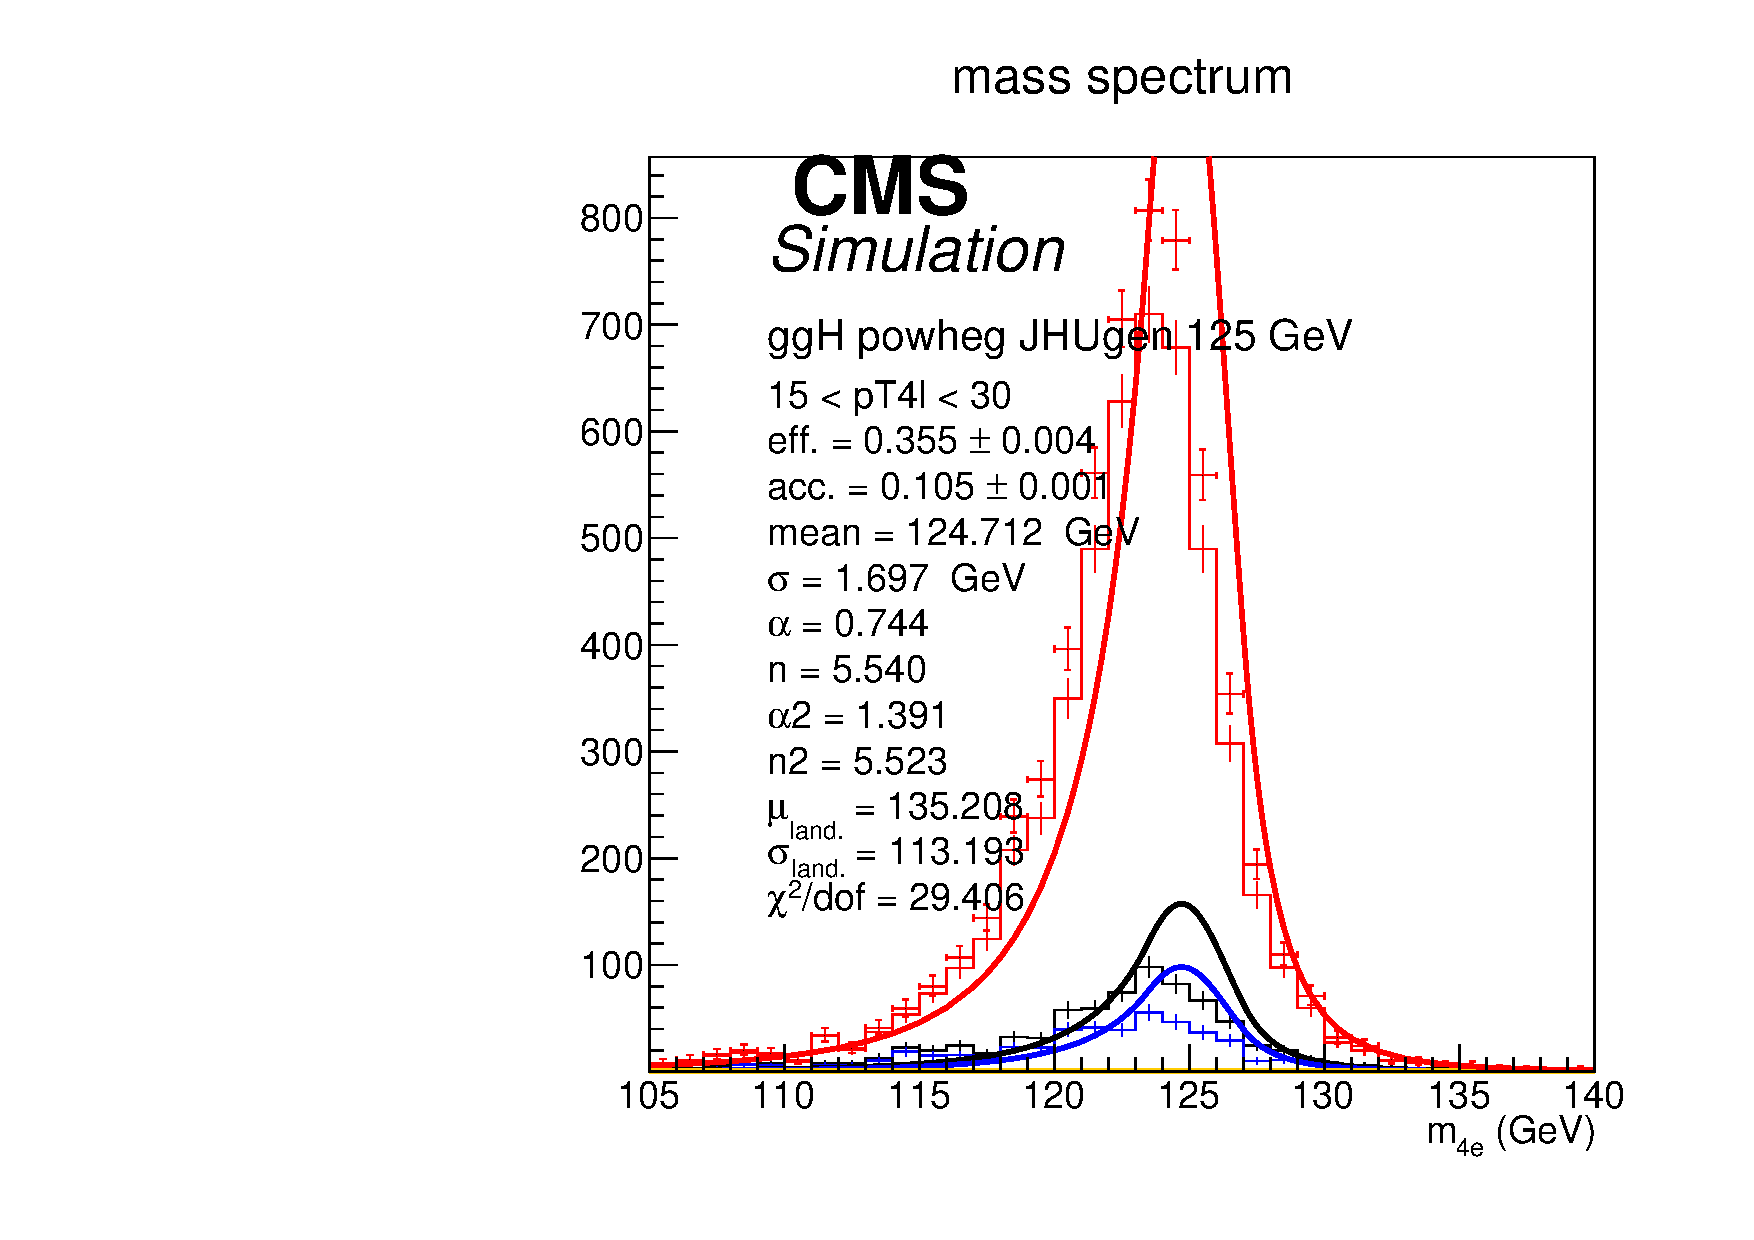
\includegraphics[width=0.3\textwidth,angle=0]{Figures/Appendix//ggH_powheg_JHUgen_125_4e_pT4l_genbin1_recobin1_effs_genWeight*pileupWeight*dataMCWeight.pdf}
      \label{fig:sigfits-pT4l-ggH-powheg15-JHUgen-125-maintext:b}
    }
   \subfigure[$30.0 < \pt(\mathrm{H}) < 45.0$]{
      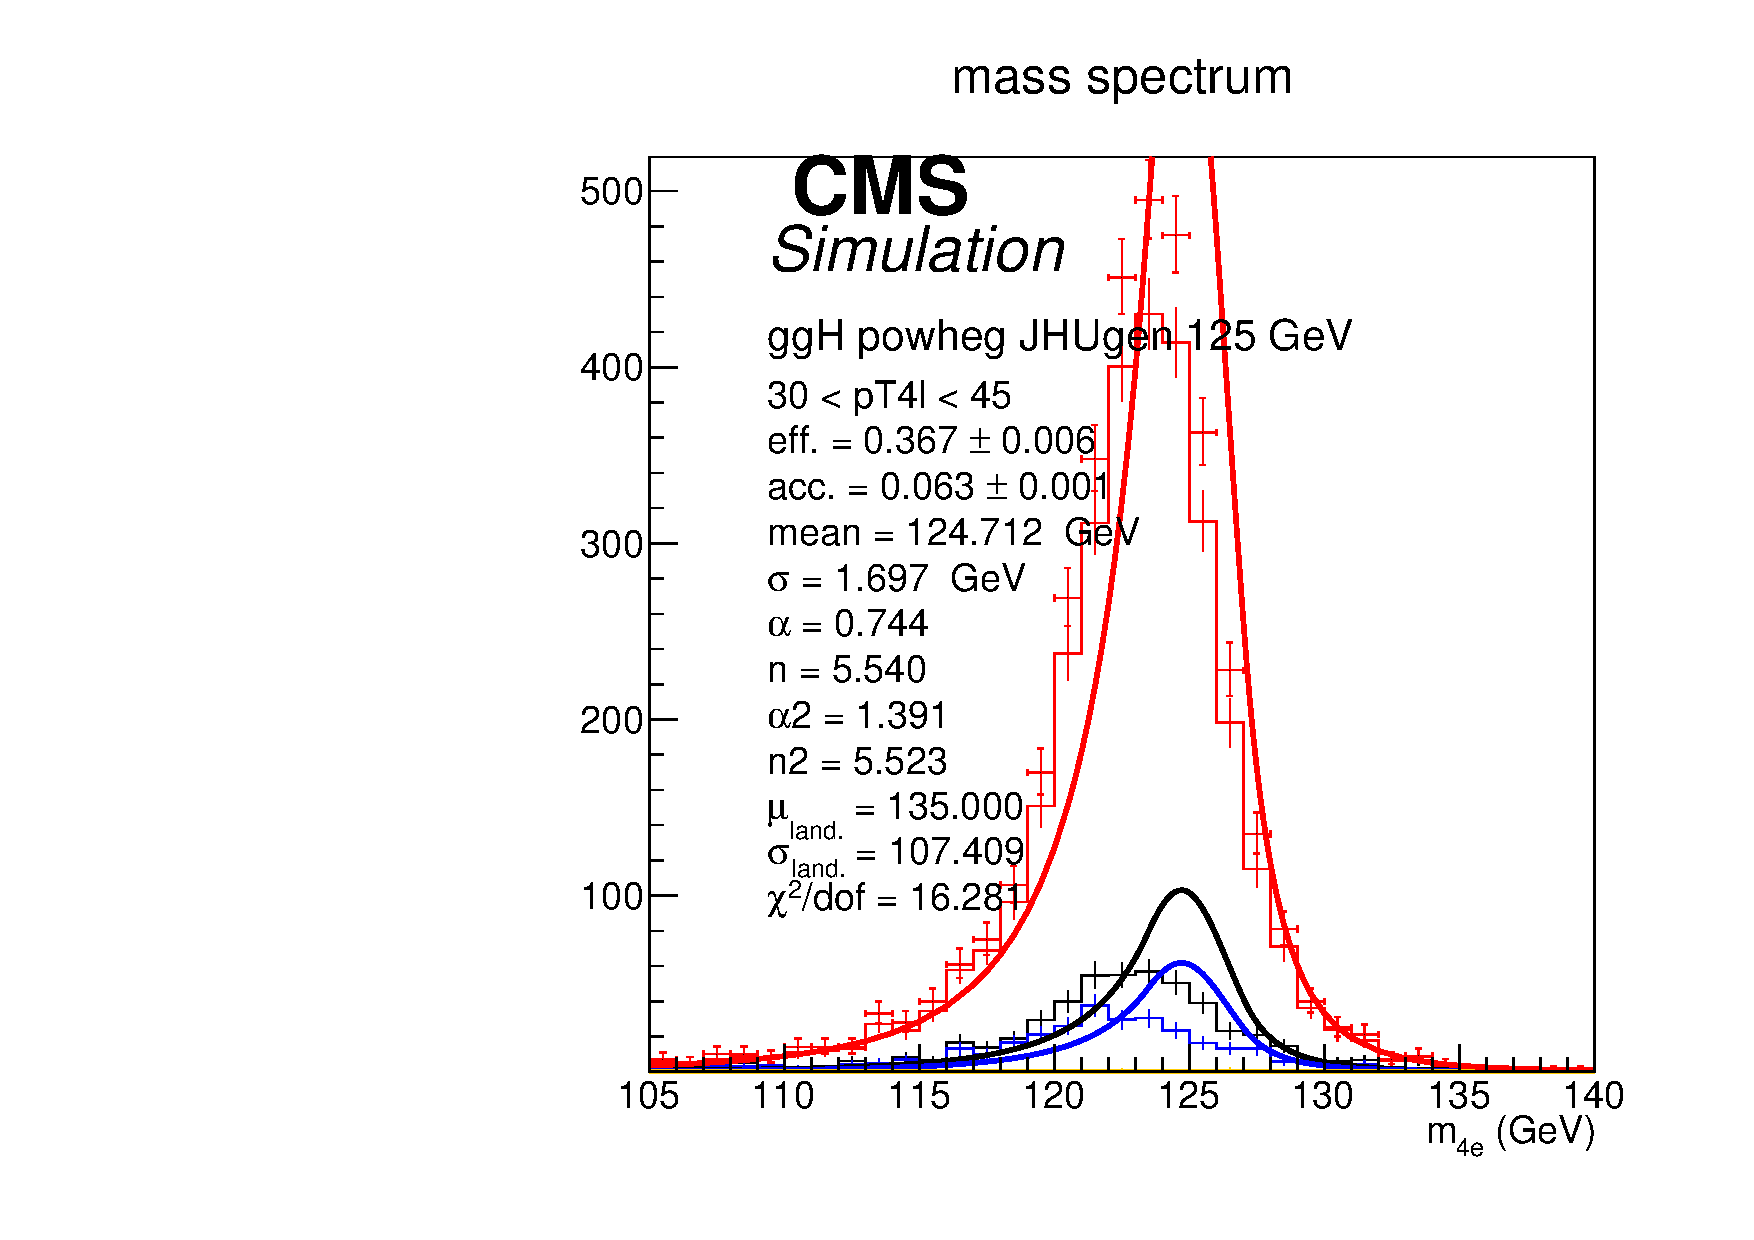
\includegraphics[width=0.3\textwidth,angle=0]{Figures/Appendix//ggH_powheg_JHUgen_125_4e_pT4l_genbin2_recobin2_effs_genWeight*pileupWeight*dataMCWeight.pdf}
      \label{fig:sigfits-pT4l-ggH-powheg15-JHUgen-125-maintext:c}
    }  \\
    \subfigure[$45.0 < \pt(\mathrm{H}) < 80.0$]{
      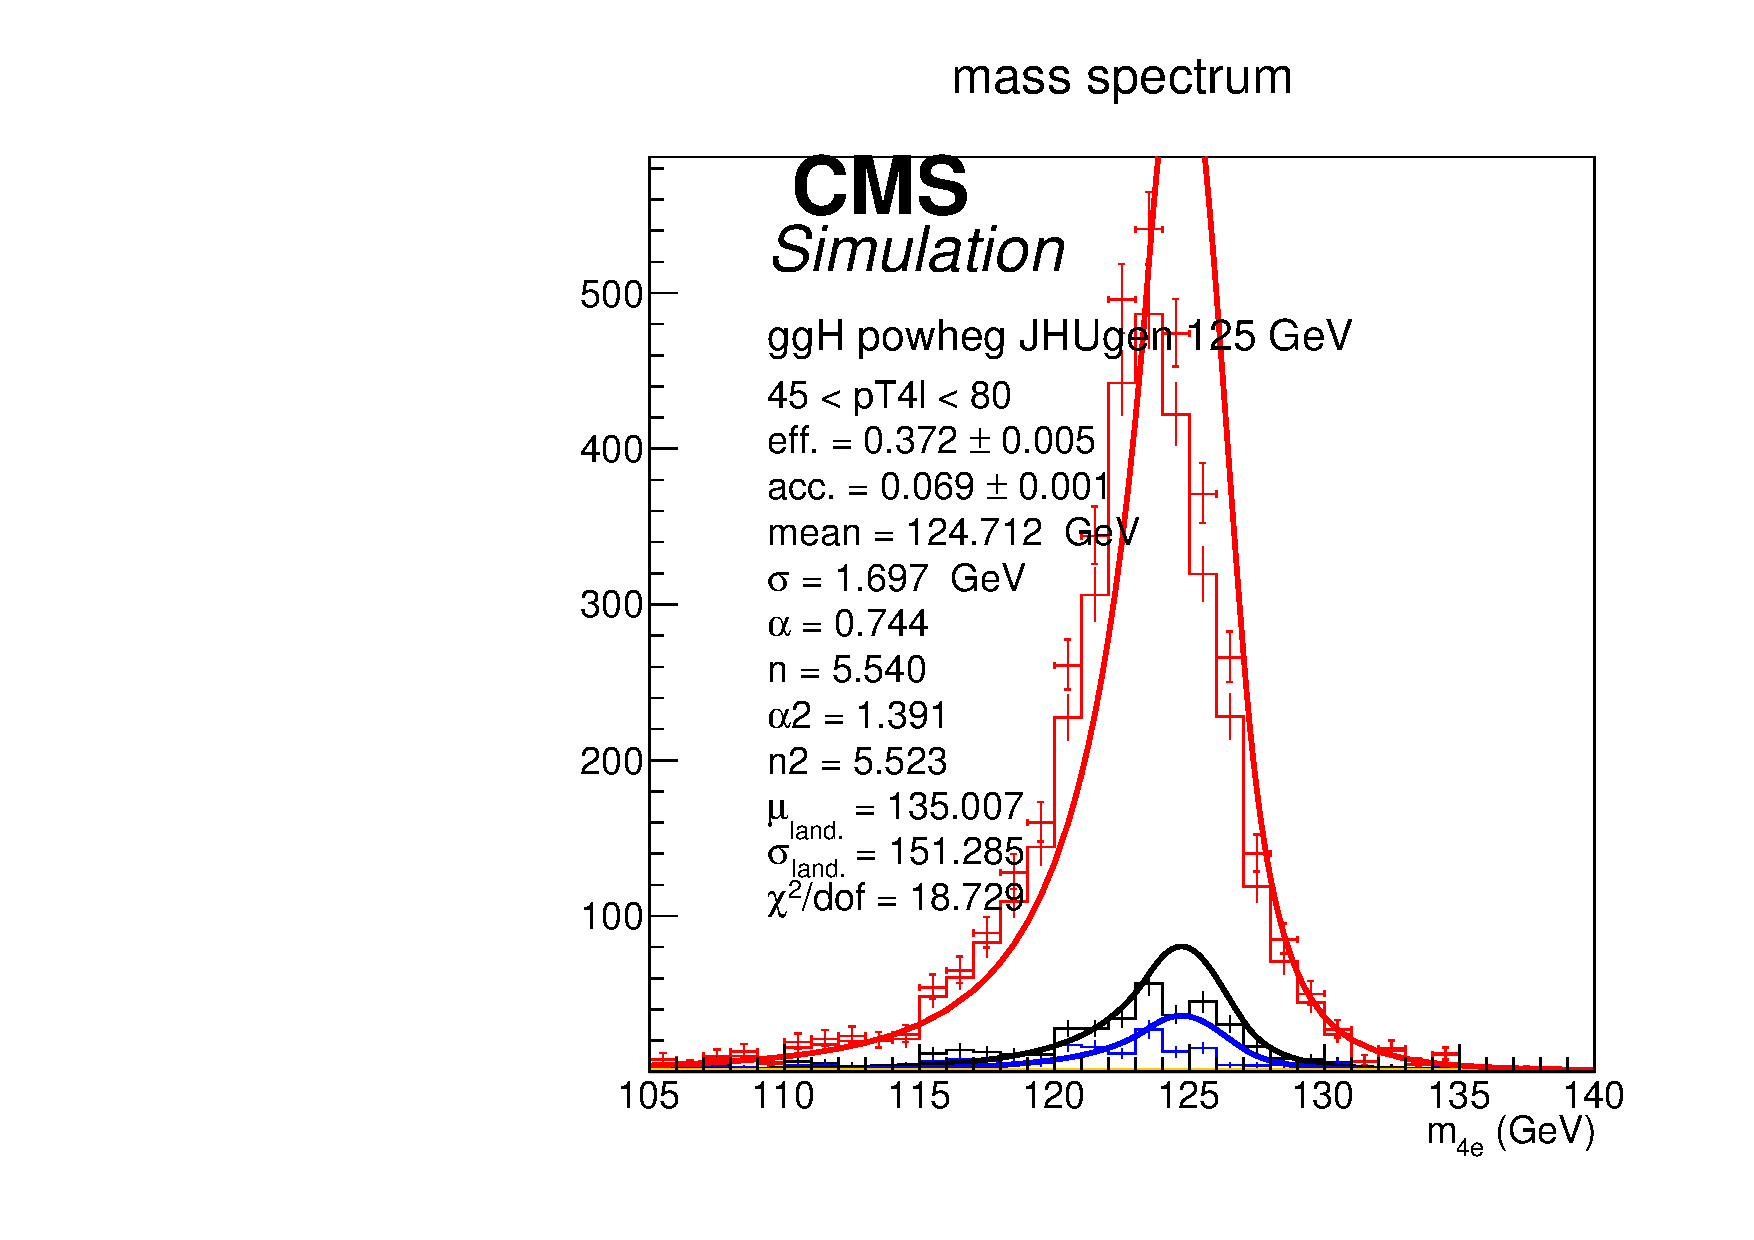
\includegraphics[width=0.3\textwidth,angle=0]{Figures/Appendix//ggH_powheg_JHUgen_125_4e_pT4l_genbin3_recobin3_effs_genWeight*pileupWeight*dataMCWeight.pdf}
      \label{fig:sigfits-pT4l-ggH-powheg15-JHUgen-125-maintext:d}
    }
    \subfigure[$80.0 < \pt(\mathrm{H}) < 120.0$]{
      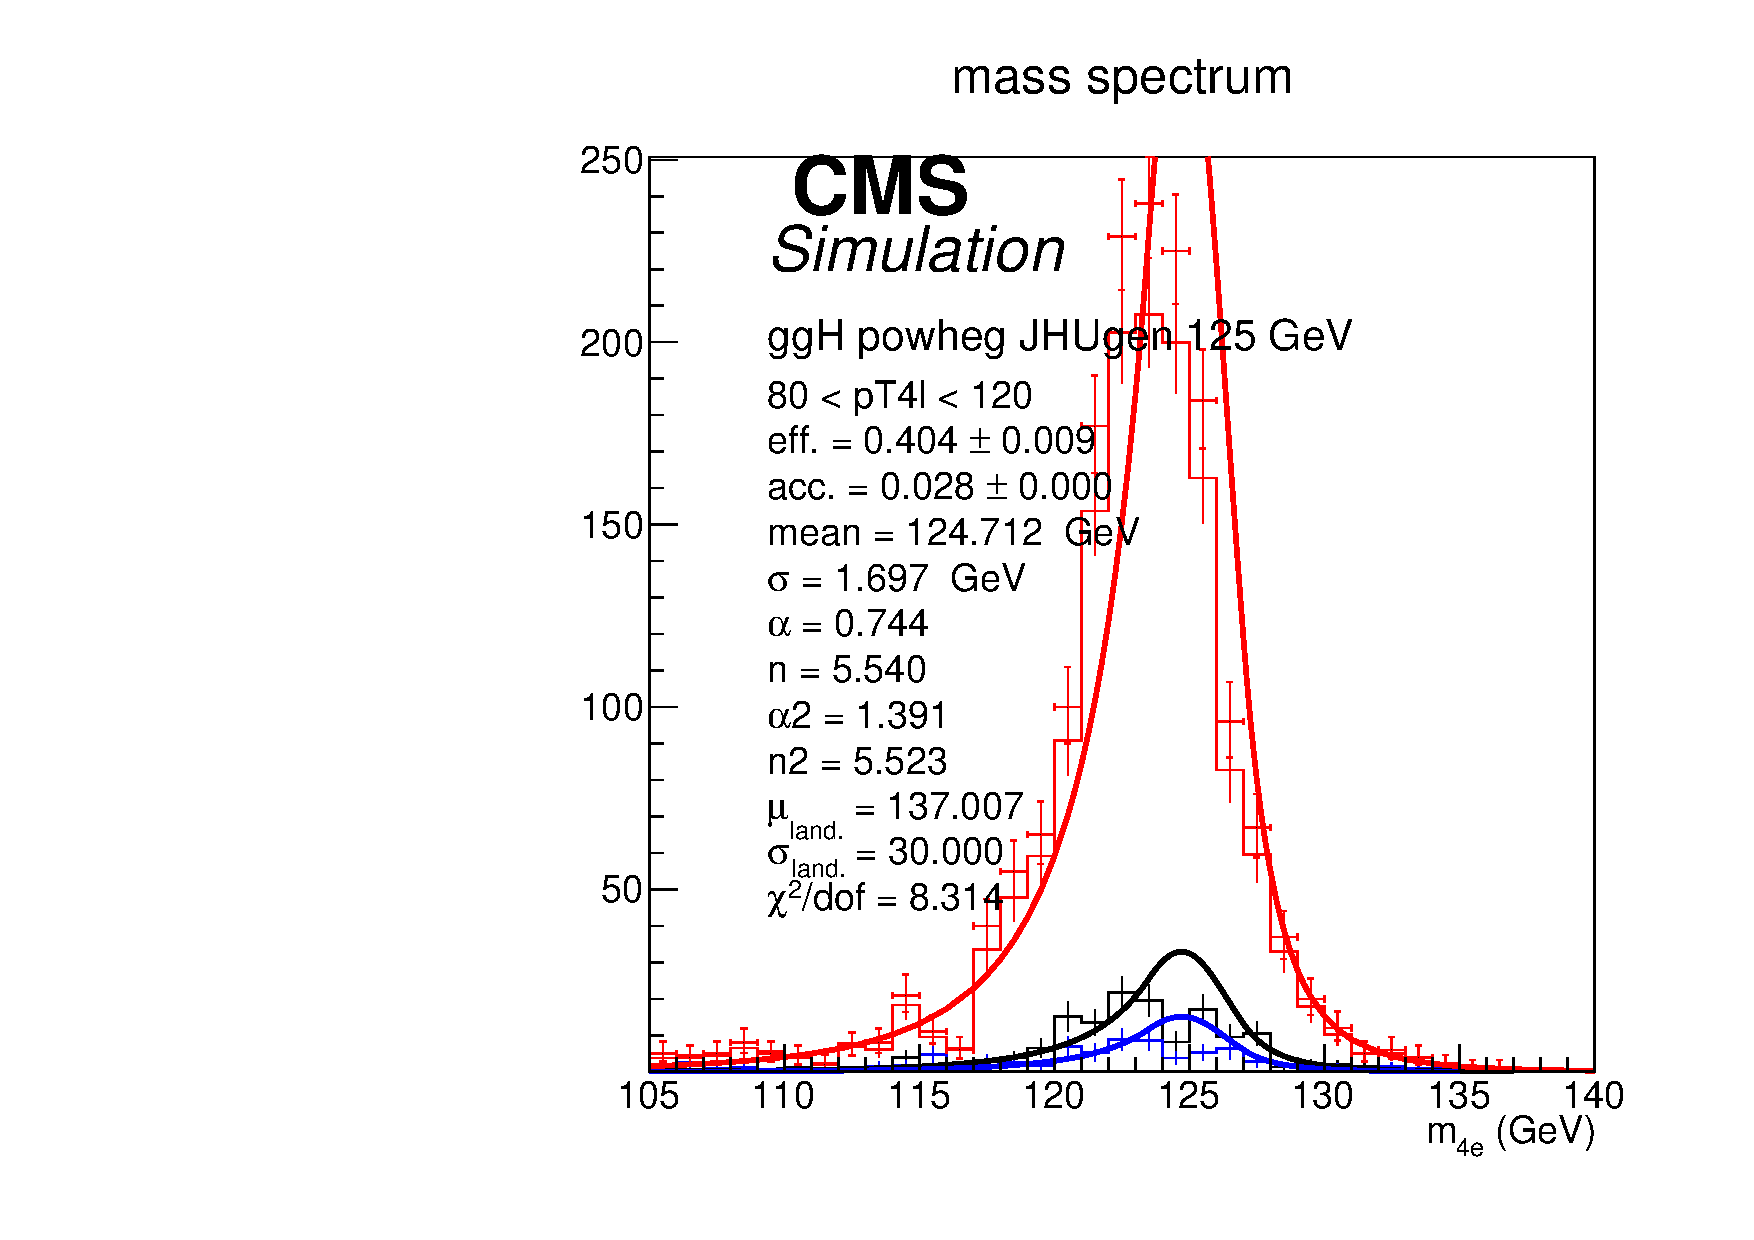
\includegraphics[width=0.3\textwidth,angle=0]{Figures/Appendix//ggH_powheg_JHUgen_125_4e_pT4l_genbin4_recobin4_effs_genWeight*pileupWeight*dataMCWeight.pdf}
      \label{fig:sigfits-pT4l-ggH-powheg15-JHUgen-125-maintext:e}
    }
    \subfigure[$120.0 < \pt(\mathrm{H}) < 200.0$]{
      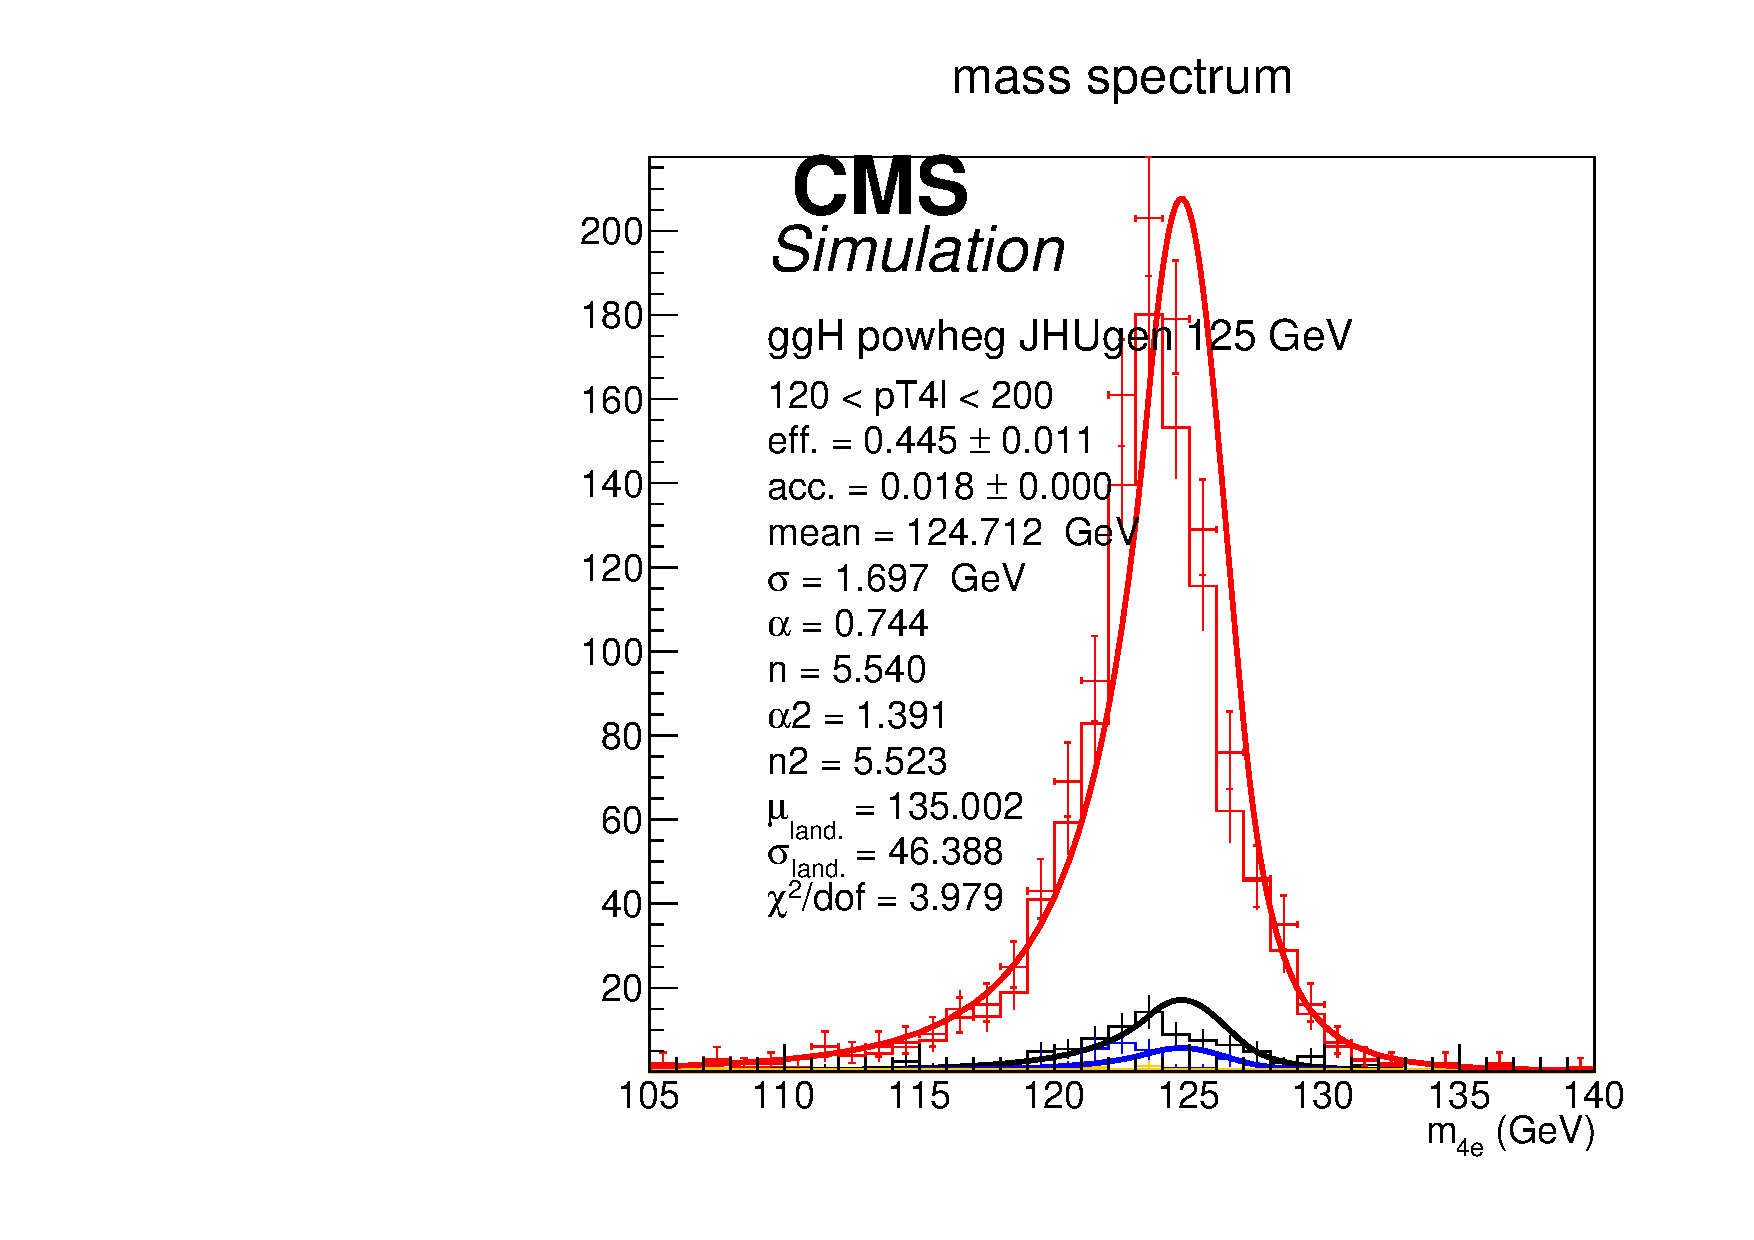
\includegraphics[width=0.3\textwidth,angle=0]{Figures/Appendix//ggH_powheg_JHUgen_125_4e_pT4l_genbin5_recobin5_effs_genWeight*pileupWeight*dataMCWeight.pdf}
      \label{fig:sigfits-pT4l-ggH-powheg15-JHUgen-125-maintext:f}
    } \\
    \subfigure[$200.0 < \pt(\mathrm{H}) < 13000.0$]{
      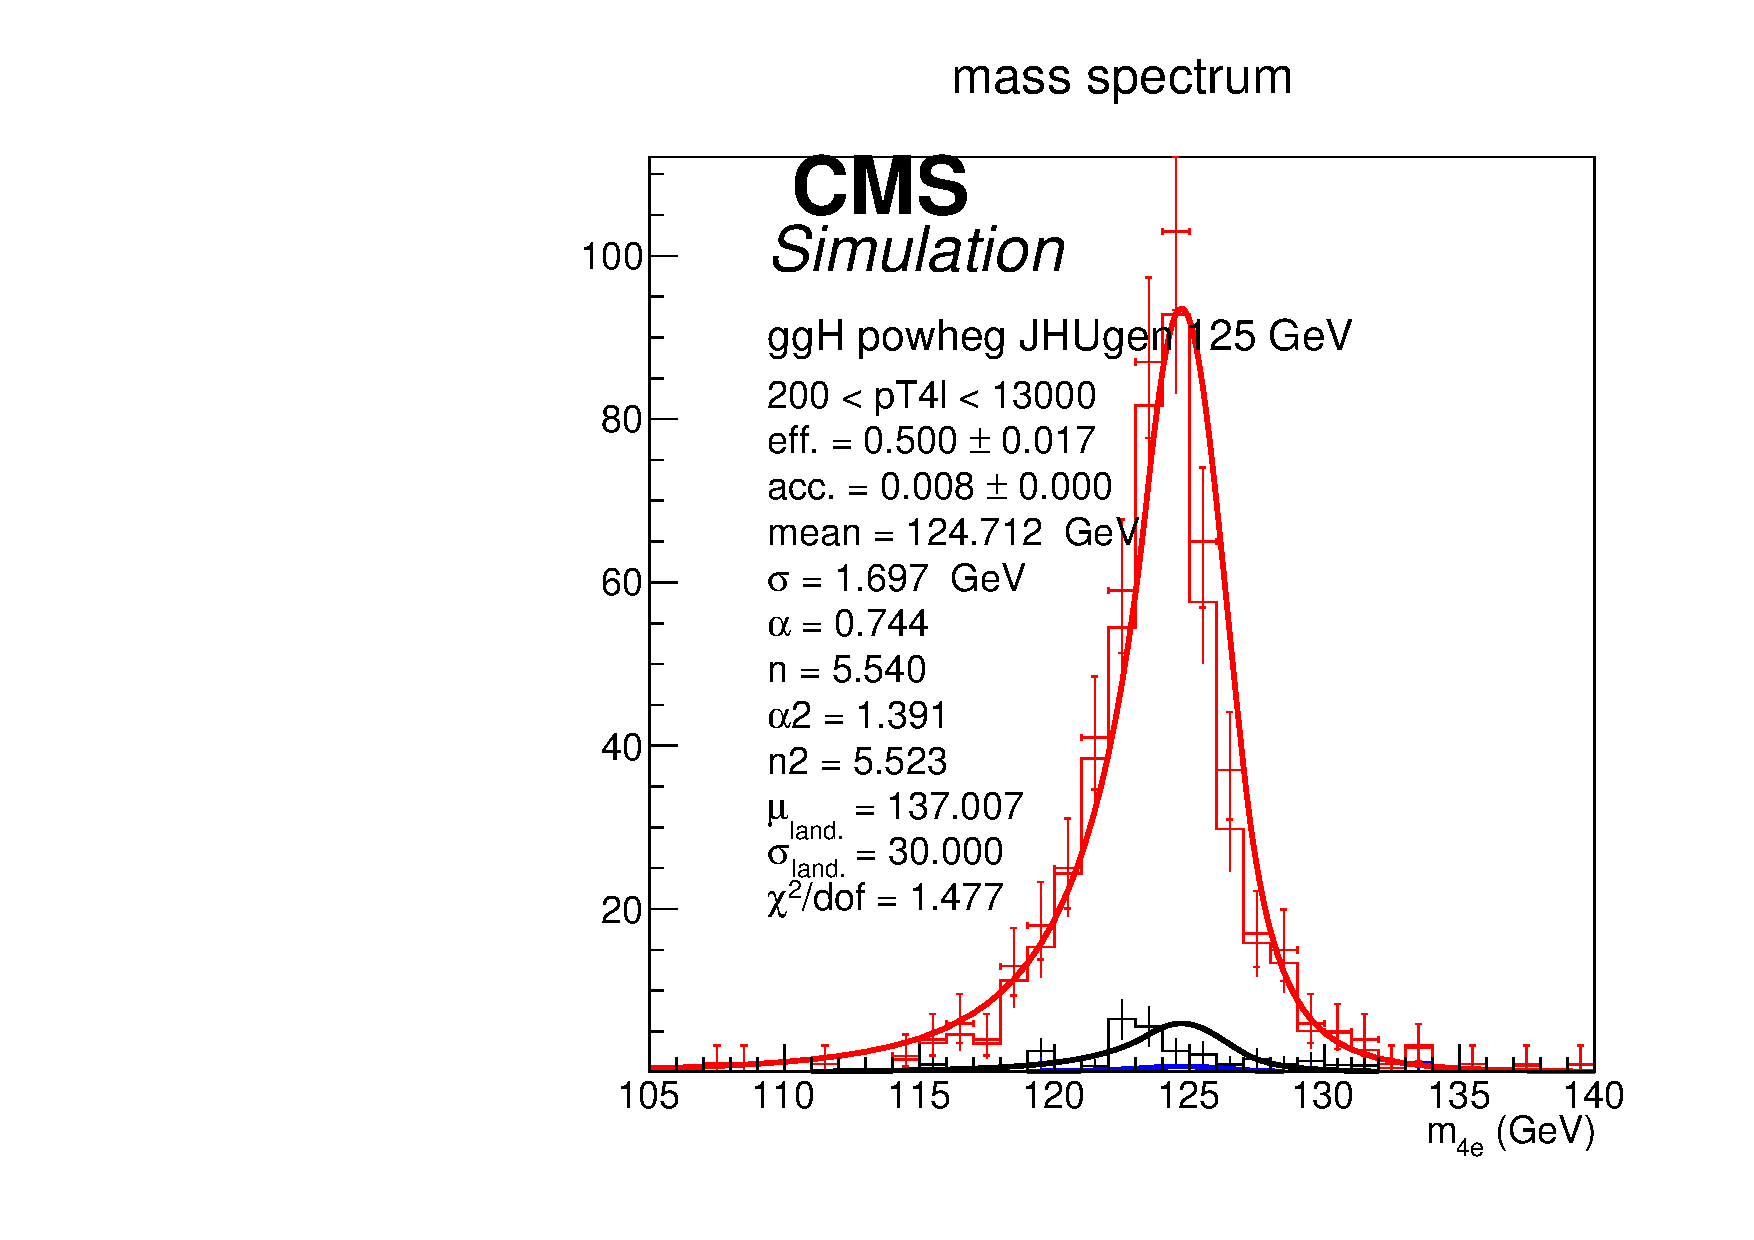
\includegraphics[width=0.3\textwidth,angle=0]{Figures/Appendix//ggH_powheg_JHUgen_125_4e_pT4l_genbin6_recobin6_effs_genWeight*pileupWeight*dataMCWeight.pdf}
      \label{fig:sigfits-pT4l-ggH-powheg15-JHUgen-125-maintext:g}
    }
    \\
    \caption{ Example signal shapes at reconstruction level for a resonance of m(4$\ell$) in $4e$ final state for the $gg\rightarrow \mathrm{H}$ production mode from {\sc powheg+JHUGen} in different bins of $\pt(\mathrm{H})$. The black curve represents events which do not pass the fiducial volume selection. The curve has no effect on the result.
    }
  \label{fig:sigfits-pT4l-ggH-powheg15-JHUgen-125-maintext}
 \end{center}
\end{figure} \clearpage

%% 4mu

\begin{figure}[htb]
  \begin{center}
    \subfigure[$0.0 < \pt(\mathrm{H}) < 15.0 $]{
      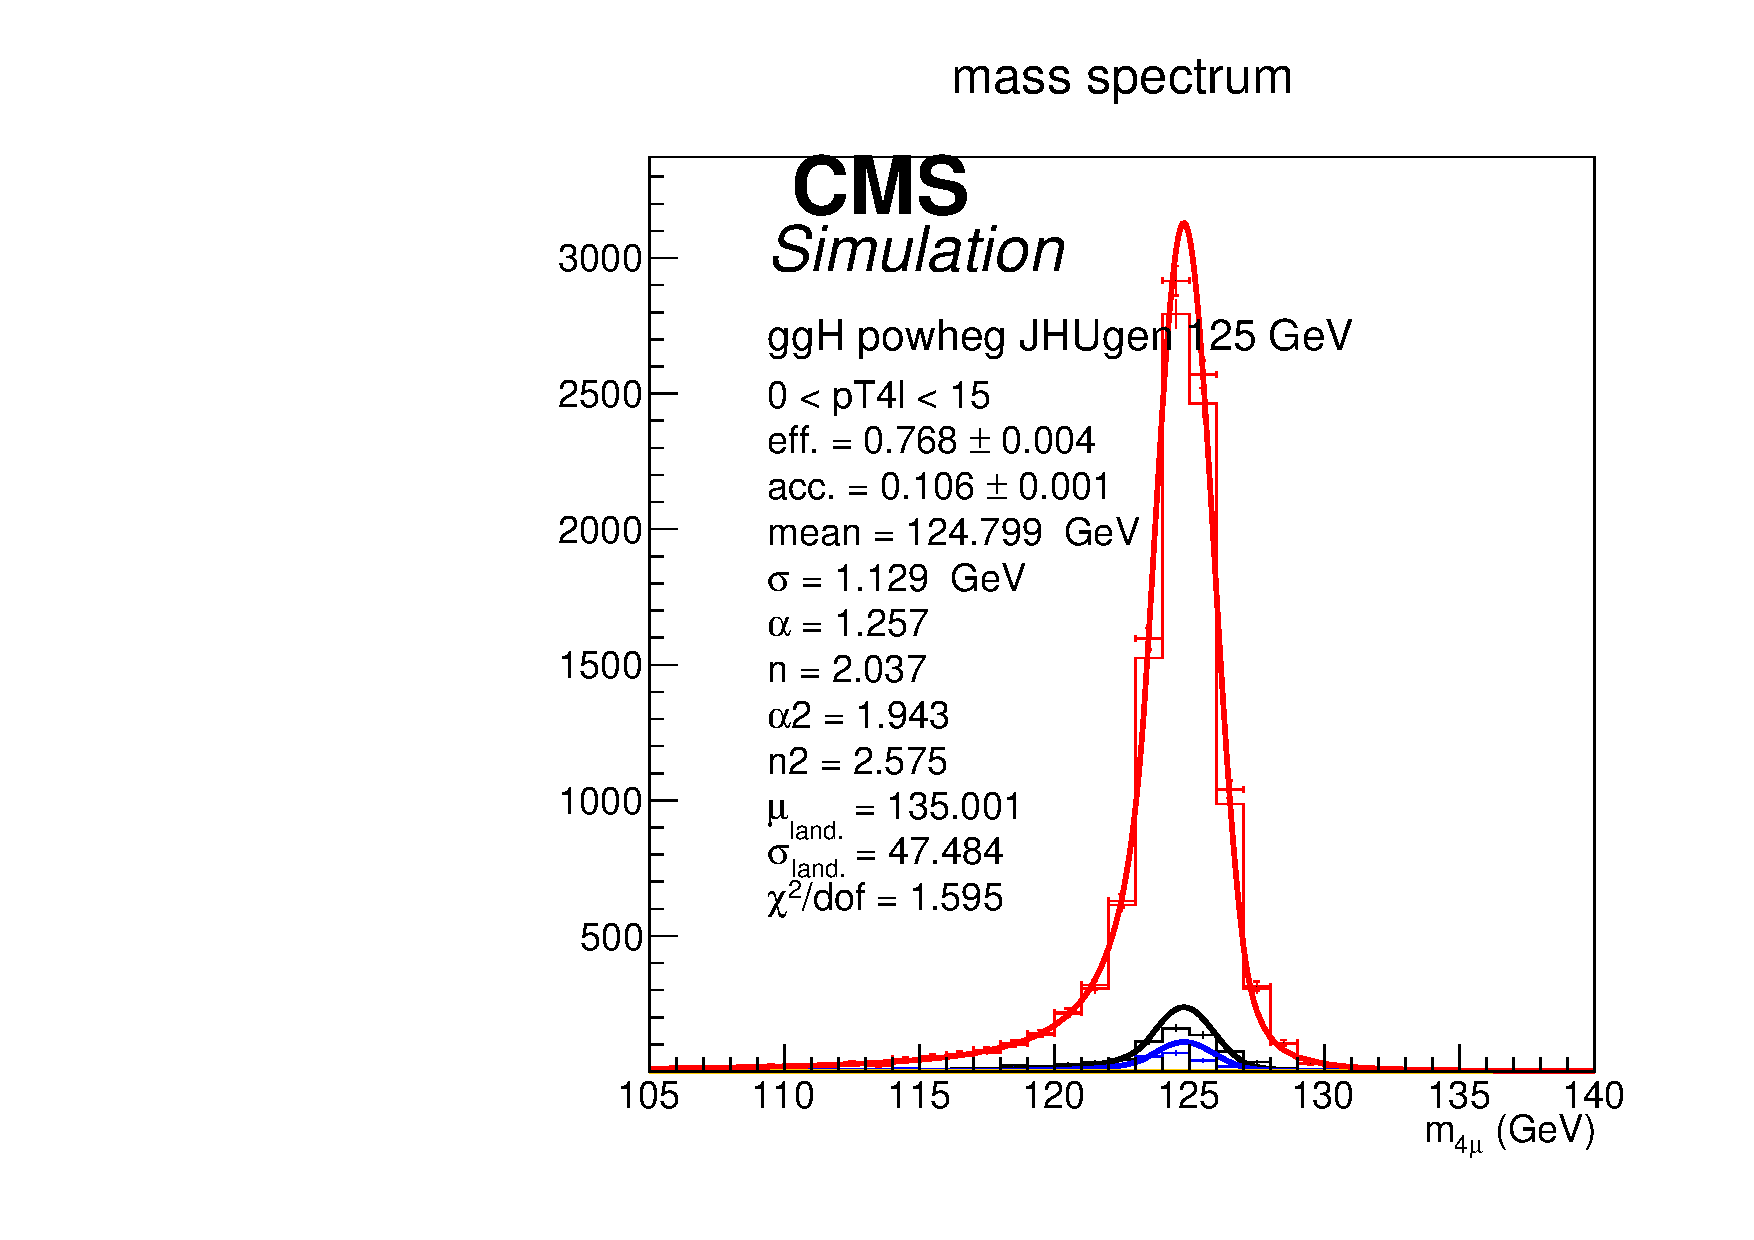
\includegraphics[width=0.3\textwidth,angle=0]{Figures/Appendix//ggH_powheg_JHUgen_125_4mu_pT4l_genbin0_recobin0_effs_genWeight*pileupWeight*dataMCWeight.pdf}
      \label{fig:sigfits-pT4l-ggH-powheg15-JHUgen-125-maintext:a}
    }
    \subfigure[$15.0 < \pt(\mathrm{H}) < 30.0$]{
      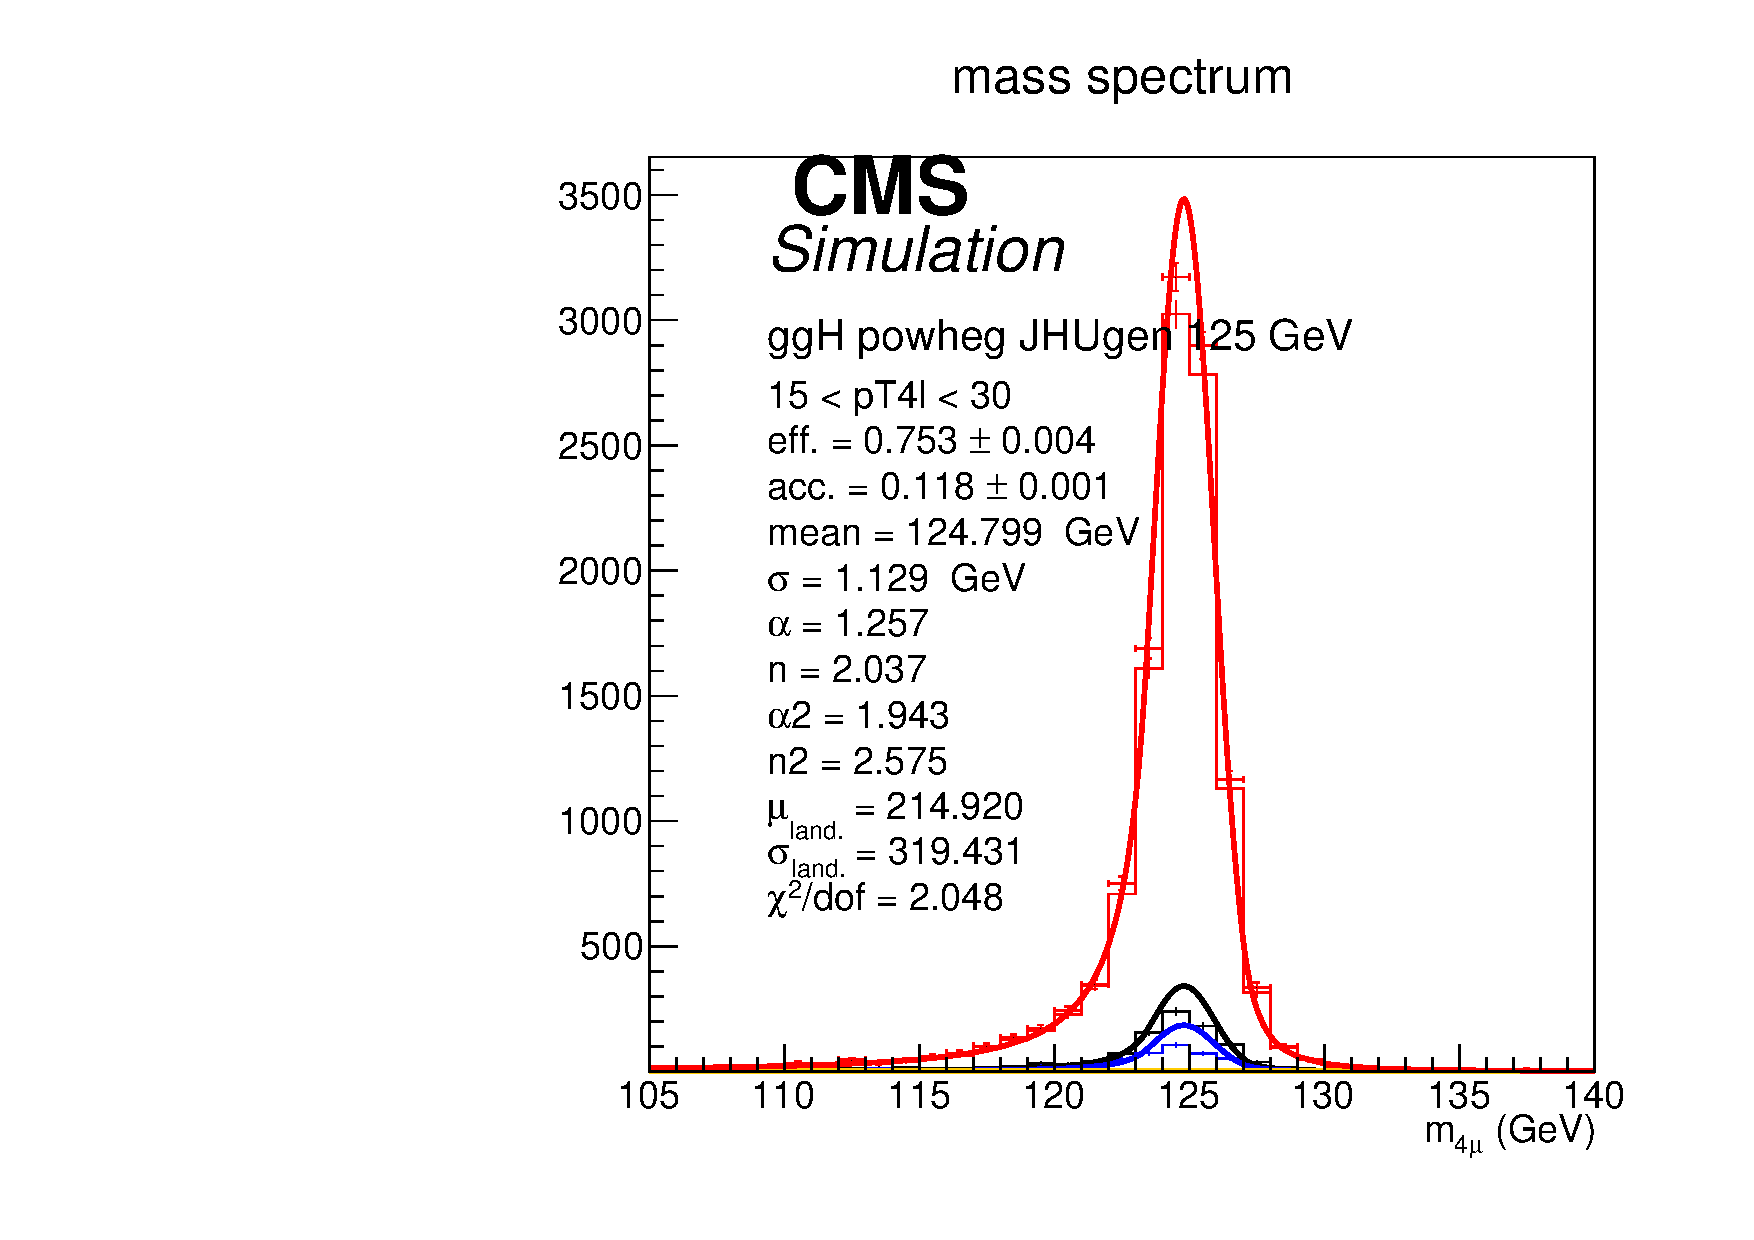
\includegraphics[width=0.3\textwidth,angle=0]{Figures/Appendix//ggH_powheg_JHUgen_125_4mu_pT4l_genbin1_recobin1_effs_genWeight*pileupWeight*dataMCWeight.pdf}
      \label{fig:sigfits-pT4l-ggH-powheg15-JHUgen-125-maintext:b}
    }
   \subfigure[$30.0 < \pt(\mathrm{H}) < 45.0$]{
      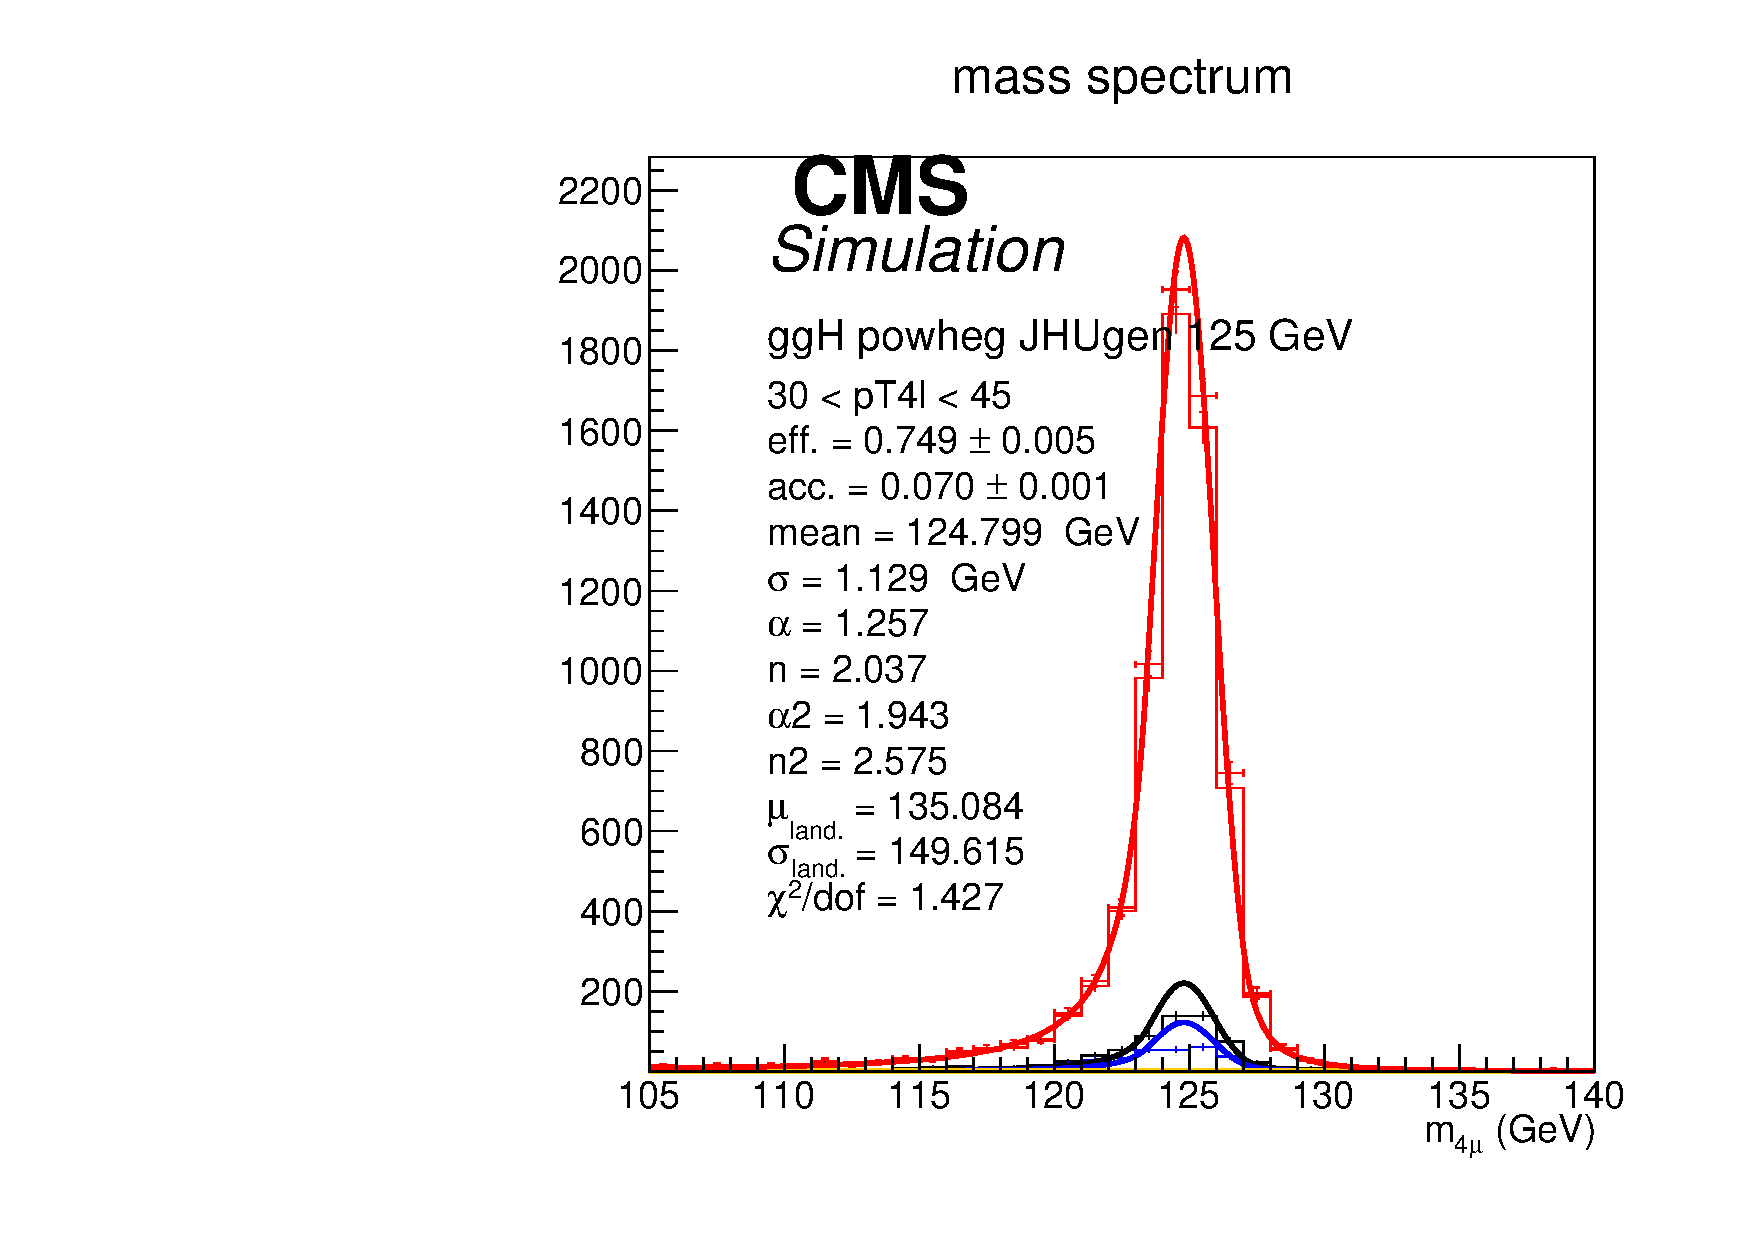
\includegraphics[width=0.3\textwidth,angle=0]{Figures/Appendix//ggH_powheg_JHUgen_125_4mu_pT4l_genbin2_recobin2_effs_genWeight*pileupWeight*dataMCWeight.pdf}
      \label{fig:sigfits-pT4l-ggH-powheg15-JHUgen-125-maintext:c}
    }  \\
    \subfigure[$45.0 < \pt(\mathrm{H}) < 80.0$]{
      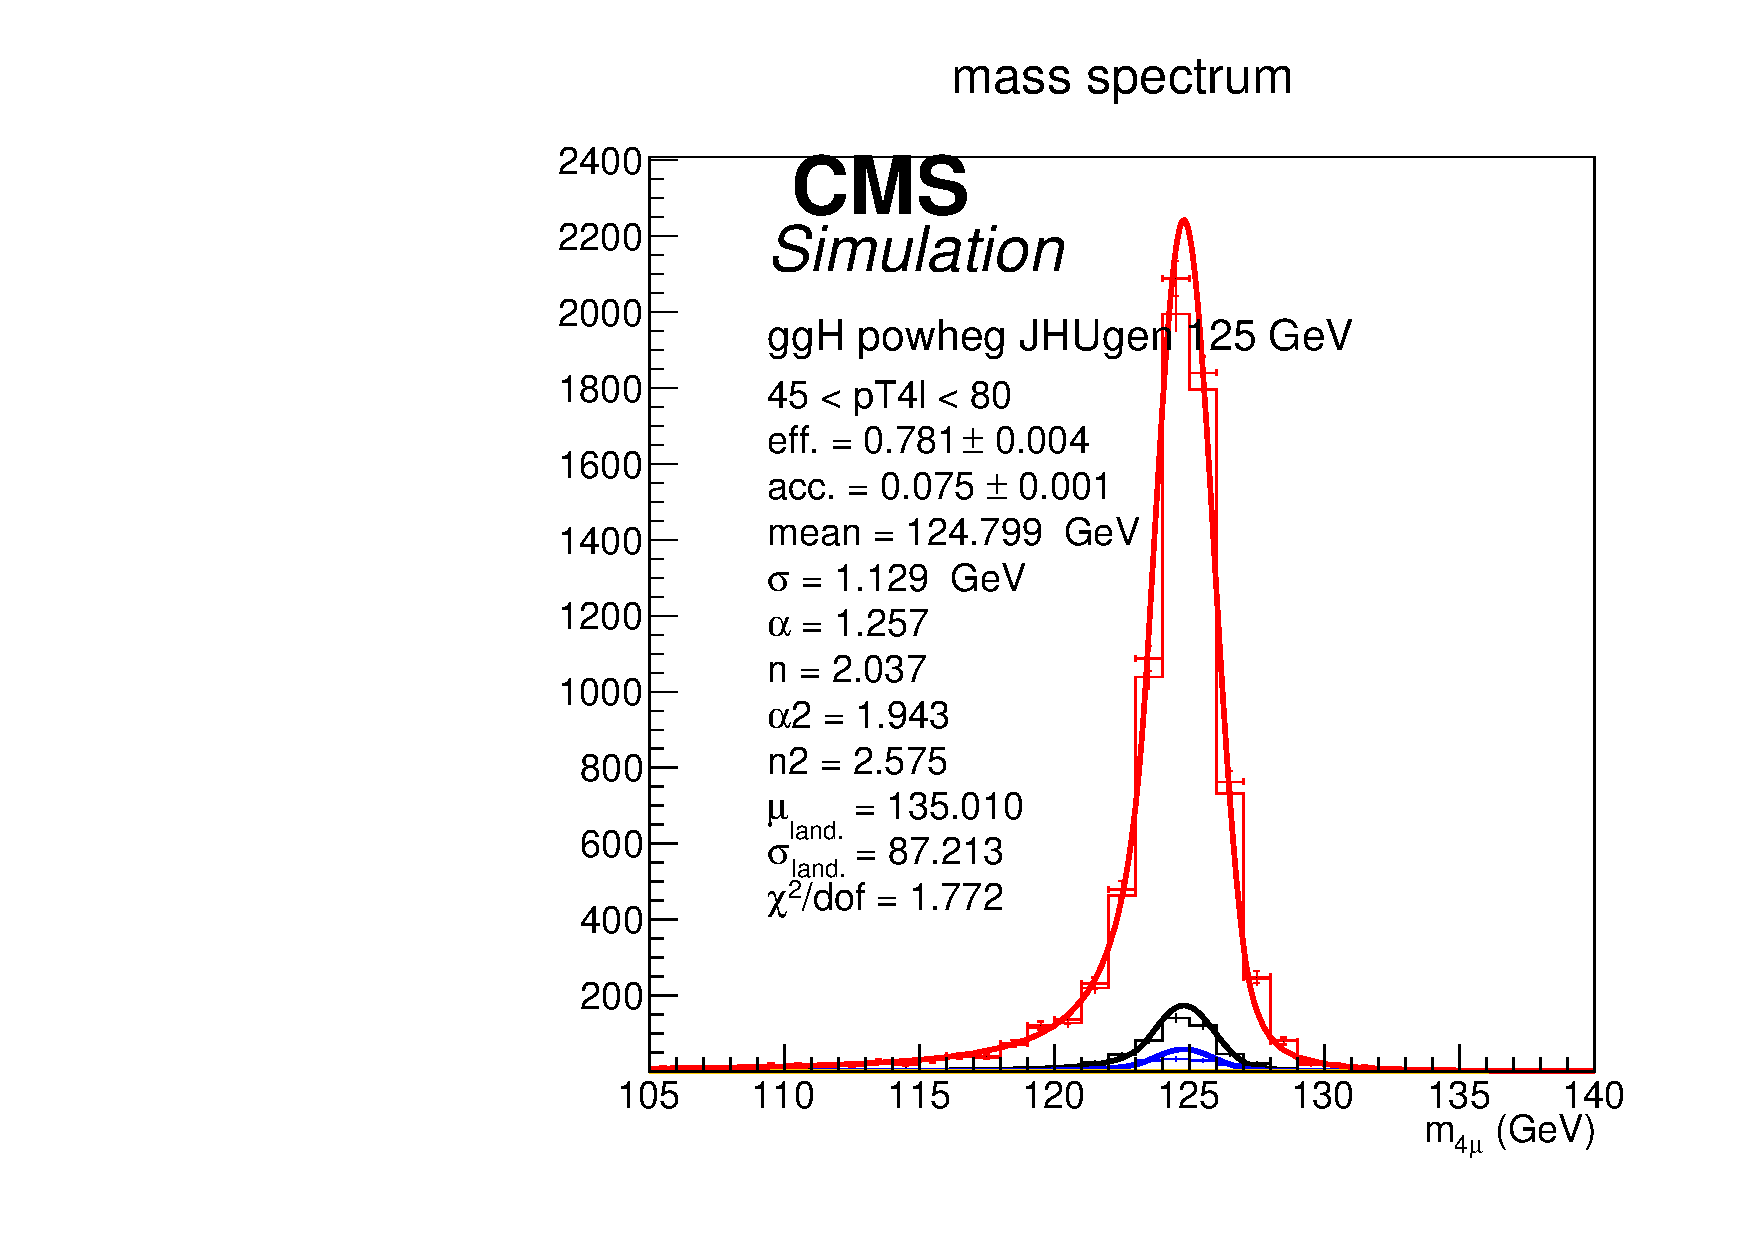
\includegraphics[width=0.3\textwidth,angle=0]{Figures/Appendix//ggH_powheg_JHUgen_125_4mu_pT4l_genbin3_recobin3_effs_genWeight*pileupWeight*dataMCWeight.pdf}
      \label{fig:sigfits-pT4l-ggH-powheg15-JHUgen-125-maintext:d}
    }
    \subfigure[$80.0 < \pt(\mathrm{H}) < 120.0$]{
      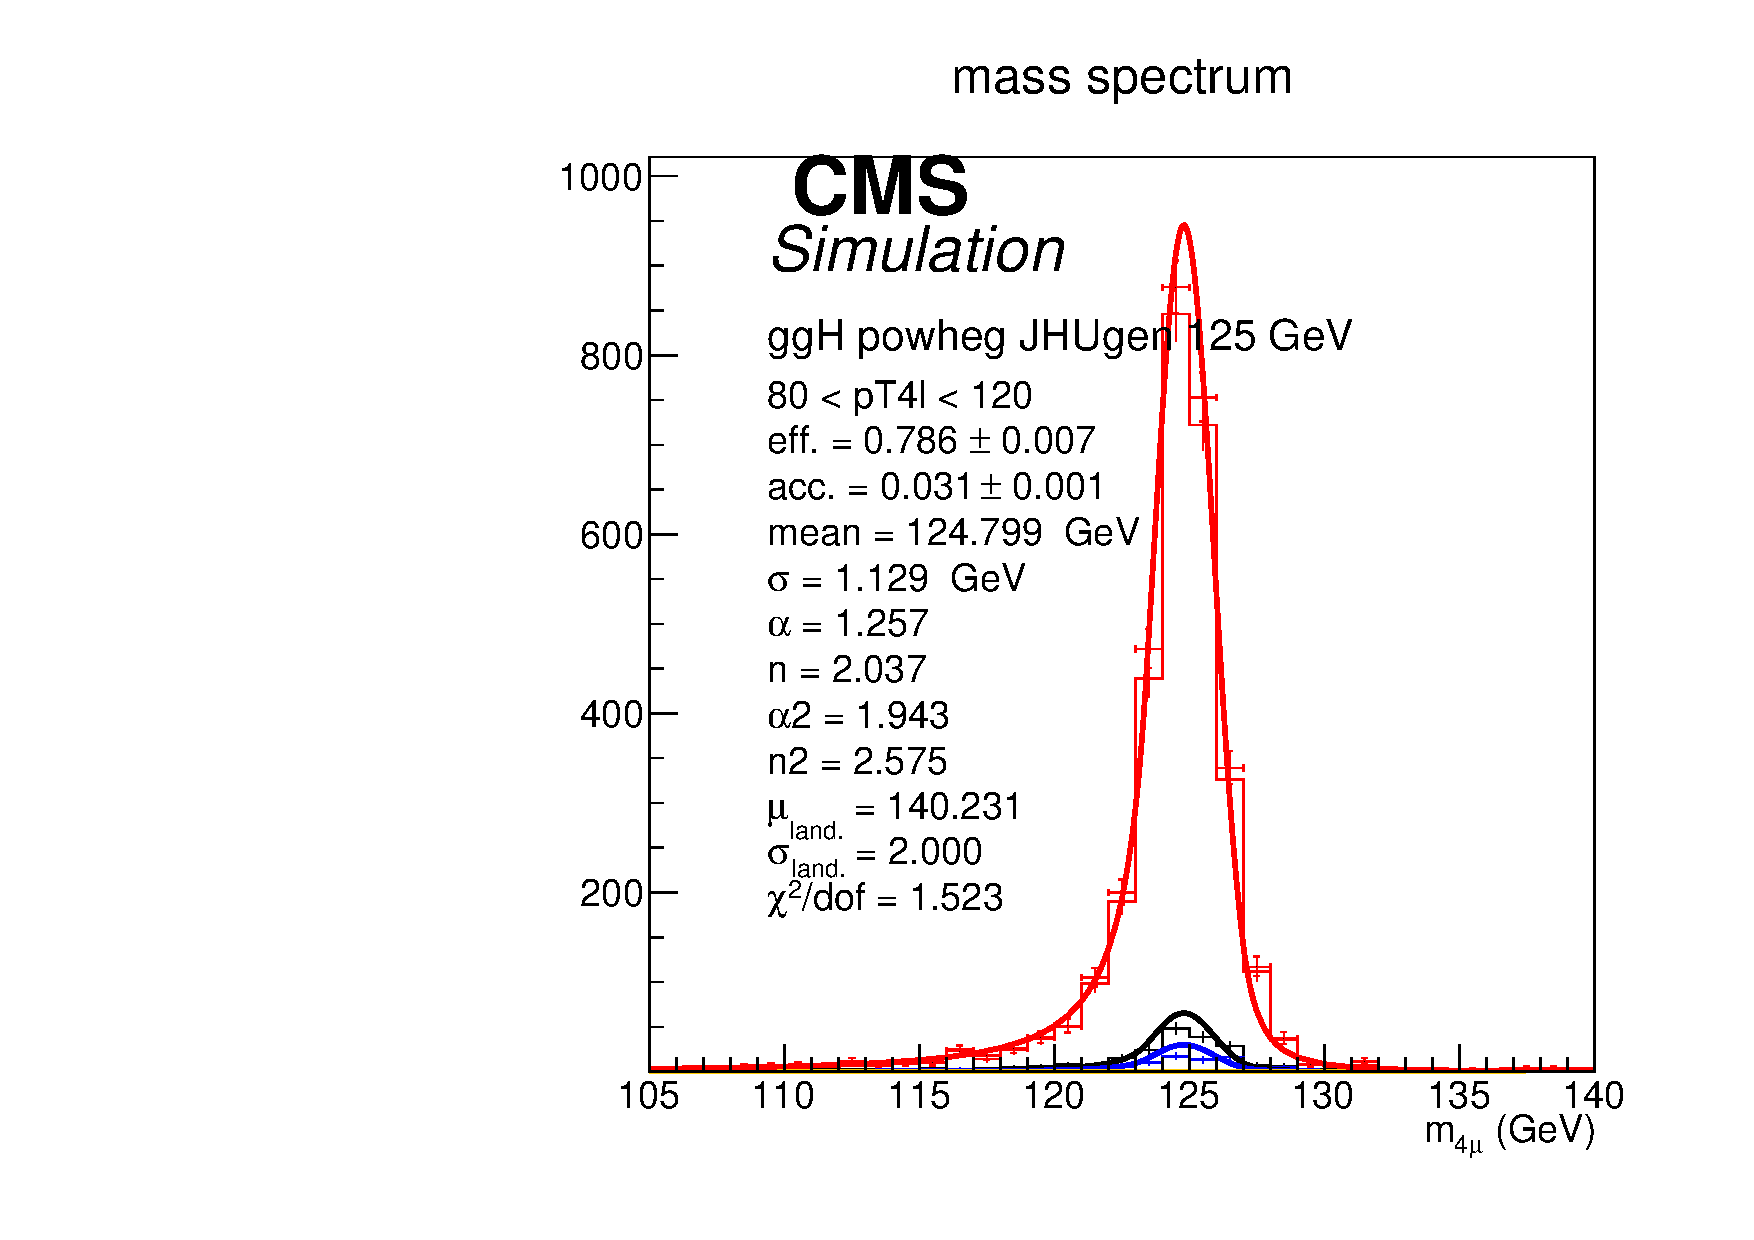
\includegraphics[width=0.3\textwidth,angle=0]{Figures/Appendix//ggH_powheg_JHUgen_125_4mu_pT4l_genbin4_recobin4_effs_genWeight*pileupWeight*dataMCWeight.pdf}
      \label{fig:sigfits-pT4l-ggH-powheg15-JHUgen-125-maintext:e}
    }
    \subfigure[$120.0 < \pt(\mathrm{H}) < 200.0$]{
      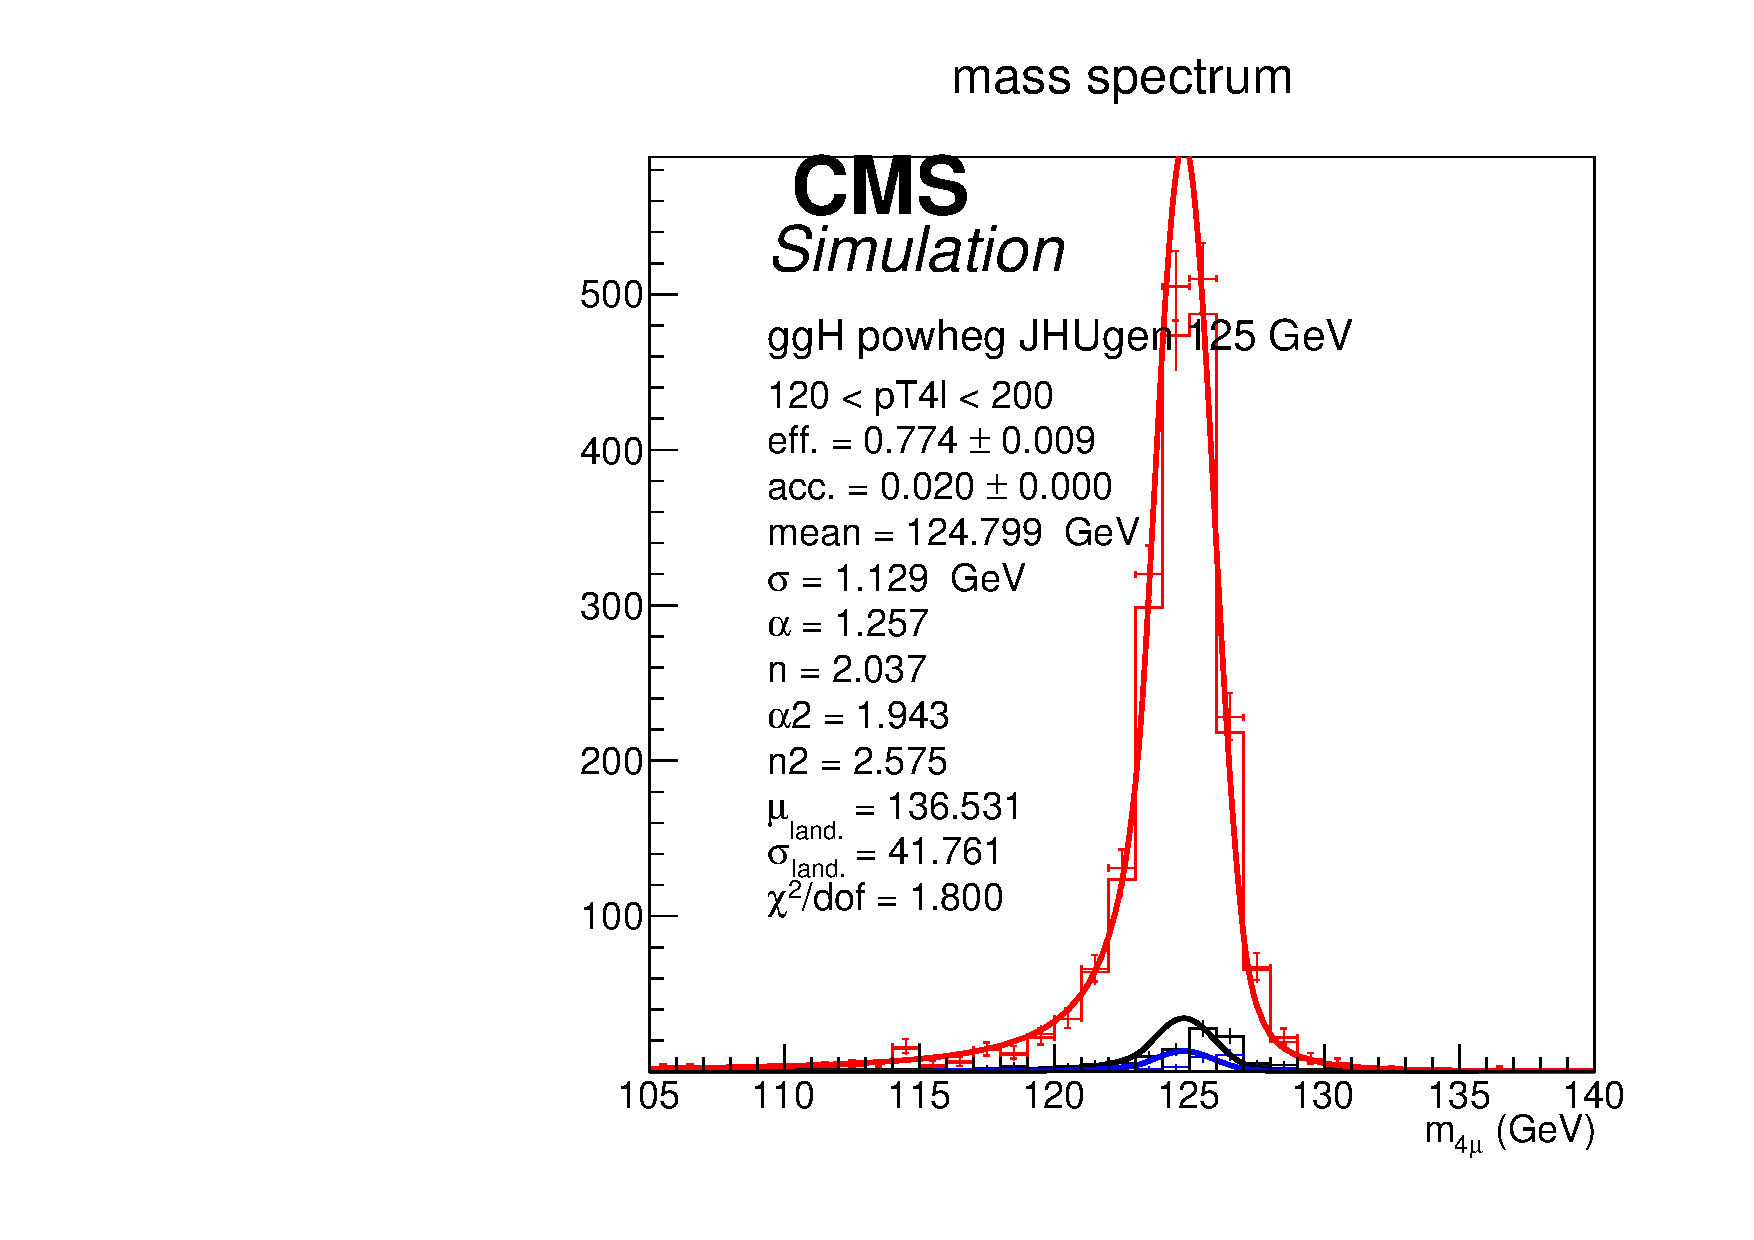
\includegraphics[width=0.3\textwidth,angle=0]{Figures/Appendix//ggH_powheg_JHUgen_125_4mu_pT4l_genbin5_recobin5_effs_genWeight*pileupWeight*dataMCWeight.pdf}
      \label{fig:sigfits-pT4l-ggH-powheg15-JHUgen-125-maintext:f}
    } \\
    \subfigure[$200.0 < \pt(\mathrm{H}) < 13000.0$]{
      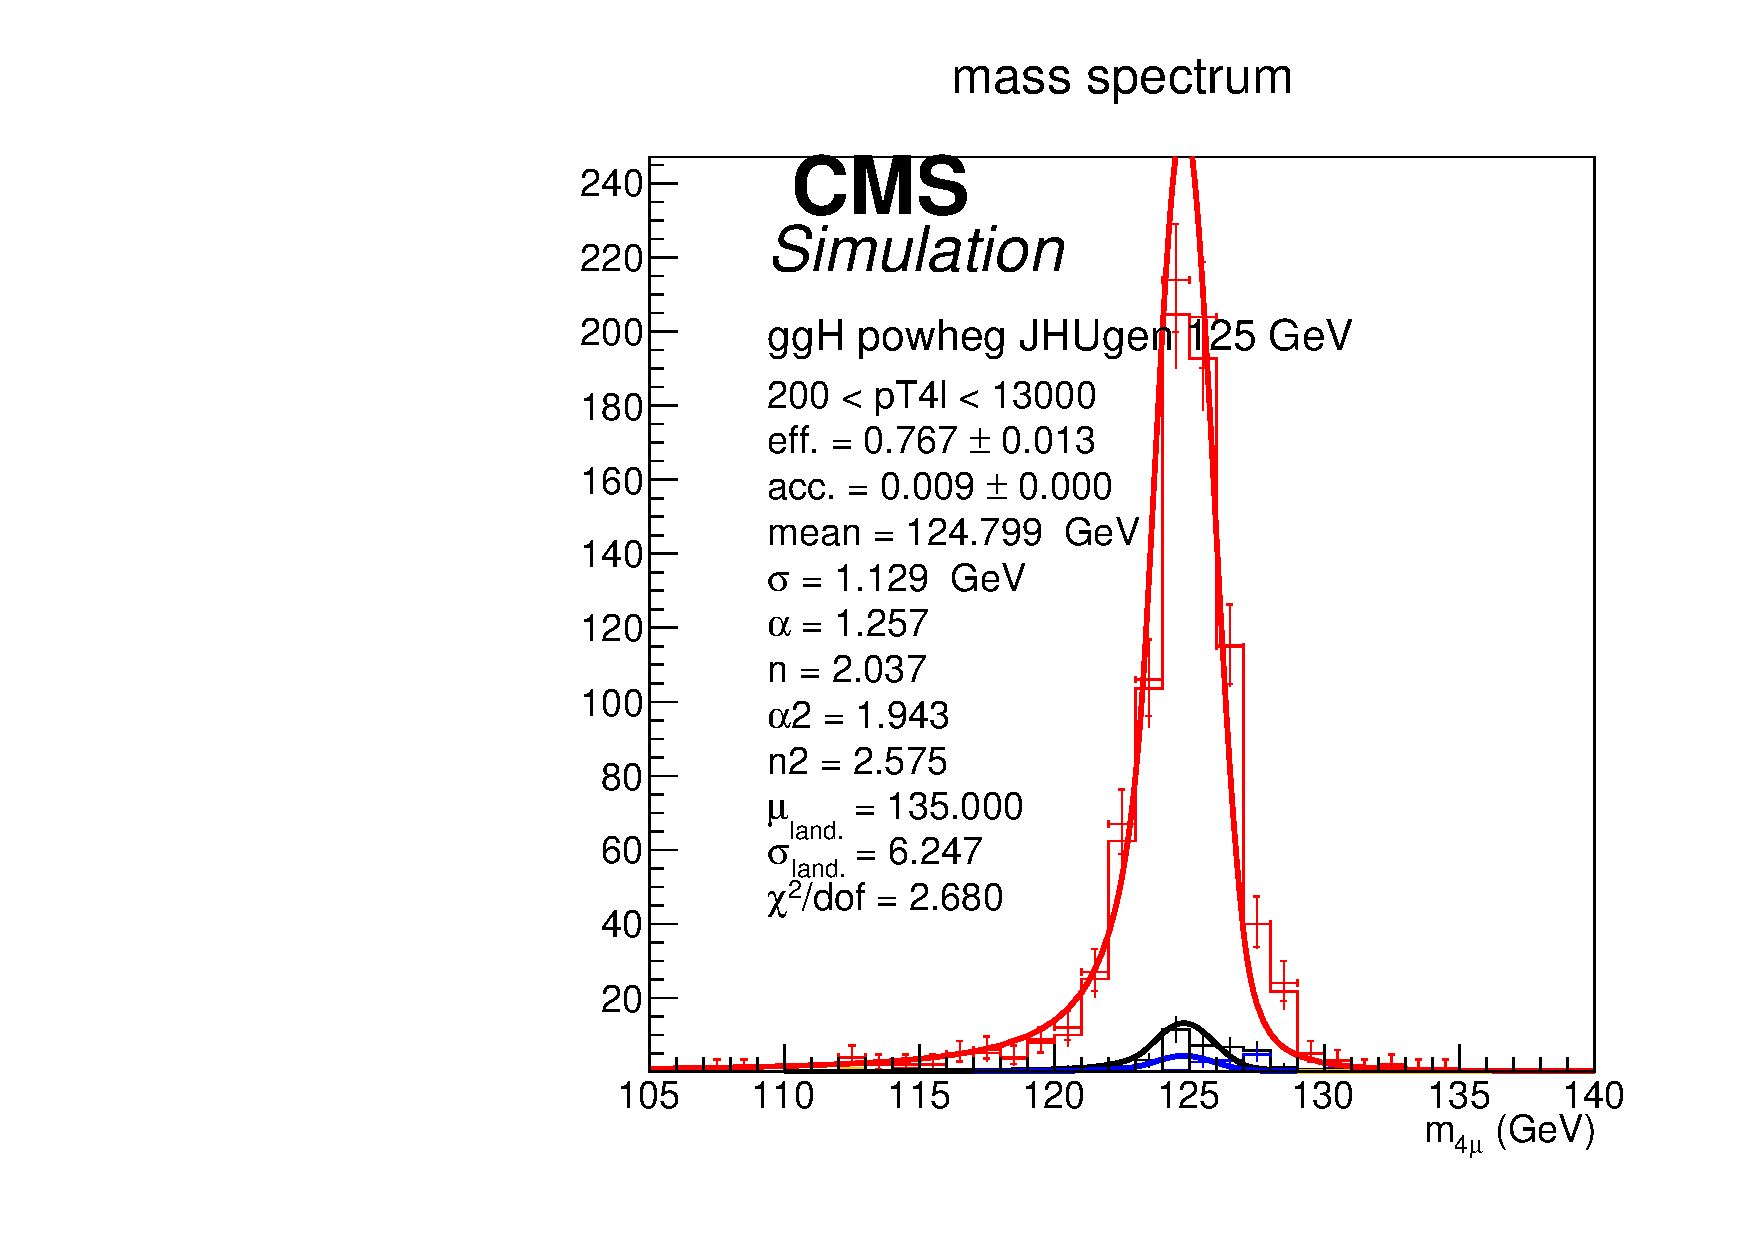
\includegraphics[width=0.3\textwidth,angle=0]{Figures/Appendix//ggH_powheg_JHUgen_125_4mu_pT4l_genbin6_recobin6_effs_genWeight*pileupWeight*dataMCWeight.pdf}
      \label{fig:sigfits-pT4l-ggH-powheg15-JHUgen-125-maintext:g}
    }
    \\
    \caption{ Example signal shapes at reconstruction level for a resonance of m(4$\ell$) in $4\mu$ final state for the $gg\rightarrow \mathrm{H}$ production mode from {\sc powheg+JHUGen} in different bins of $\pt(\mathrm{H})$. The black curve represents events which do not pass the fiducial volume selection. The curve has no effect on the result.
    }
  \label{fig:sigfits-pT4l-ggH-powheg15-JHUgen-125-maintext}
 \end{center}
\end{figure} \clearpage


%%%%%%%%%%%%%%%%%%%%%%%%%%%%%%%%%%%%%%%%%%%%%%%%%%%%%%%%%%%%% VBF %%%%%%%%%%%%%%%%%%%%%%%

\begin{figure}[htb]
  \begin{center}
    \subfigure[$0.0 < \pt(\mathrm{H}) < 15.0 $]{
      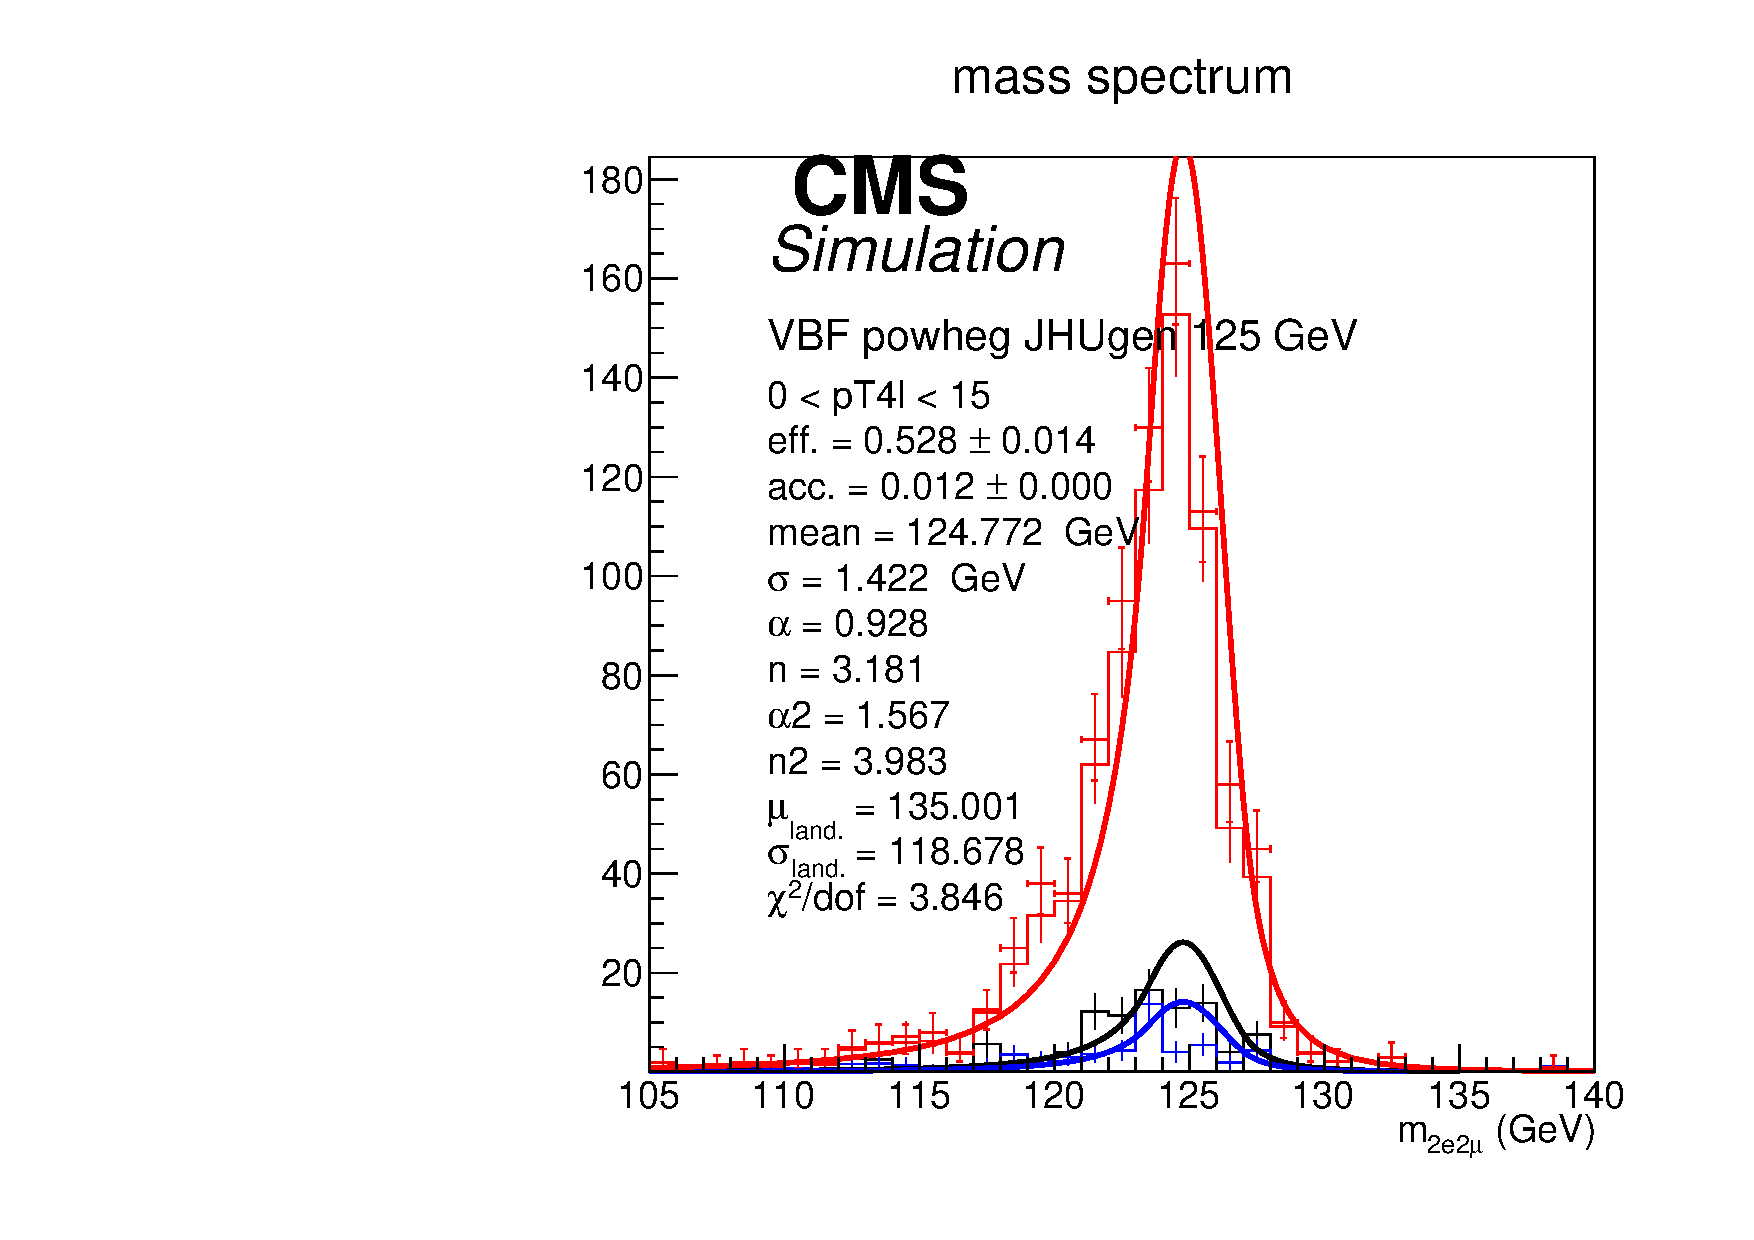
\includegraphics[width=0.3\textwidth,angle=0]{Figures/Appendix//VBF_powheg_JHUgen_125_2e2mu_pT4l_genbin0_recobin0_effs_genWeight*pileupWeight*dataMCWeight.pdf}
      \label{fig:sigfits-pT4l-VBF-powheg15-JHUgen-125-maintext:a}
    }
    \subfigure[$15.0 < \pt(\mathrm{H}) < 30.0$]{
      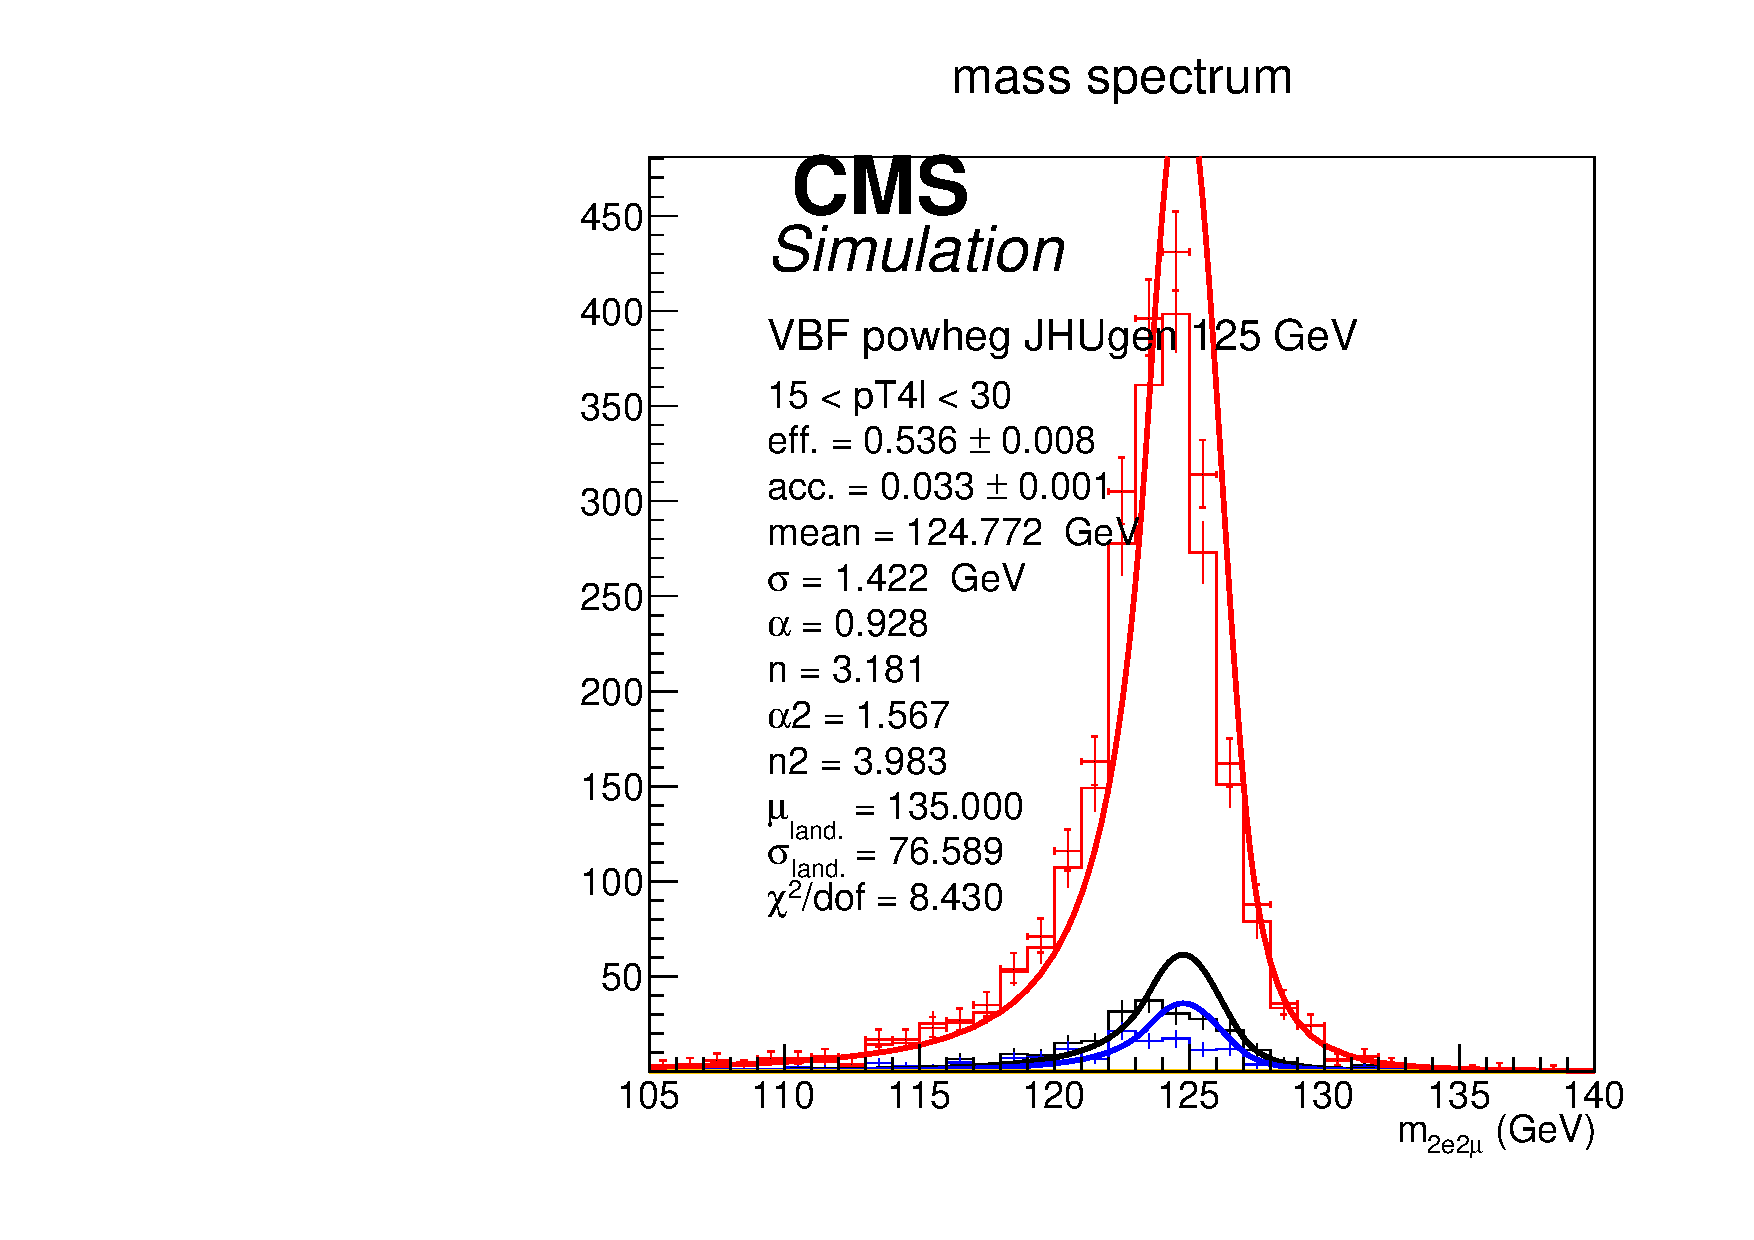
\includegraphics[width=0.3\textwidth,angle=0]{Figures/Appendix//VBF_powheg_JHUgen_125_2e2mu_pT4l_genbin1_recobin1_effs_genWeight*pileupWeight*dataMCWeight.pdf}
      \label{fig:sigfits-pT4l-VBF-powheg15-JHUgen-125-maintext:b}
    }
   \subfigure[$30.0 < \pt(\mathrm{H}) < 45.0$]{
      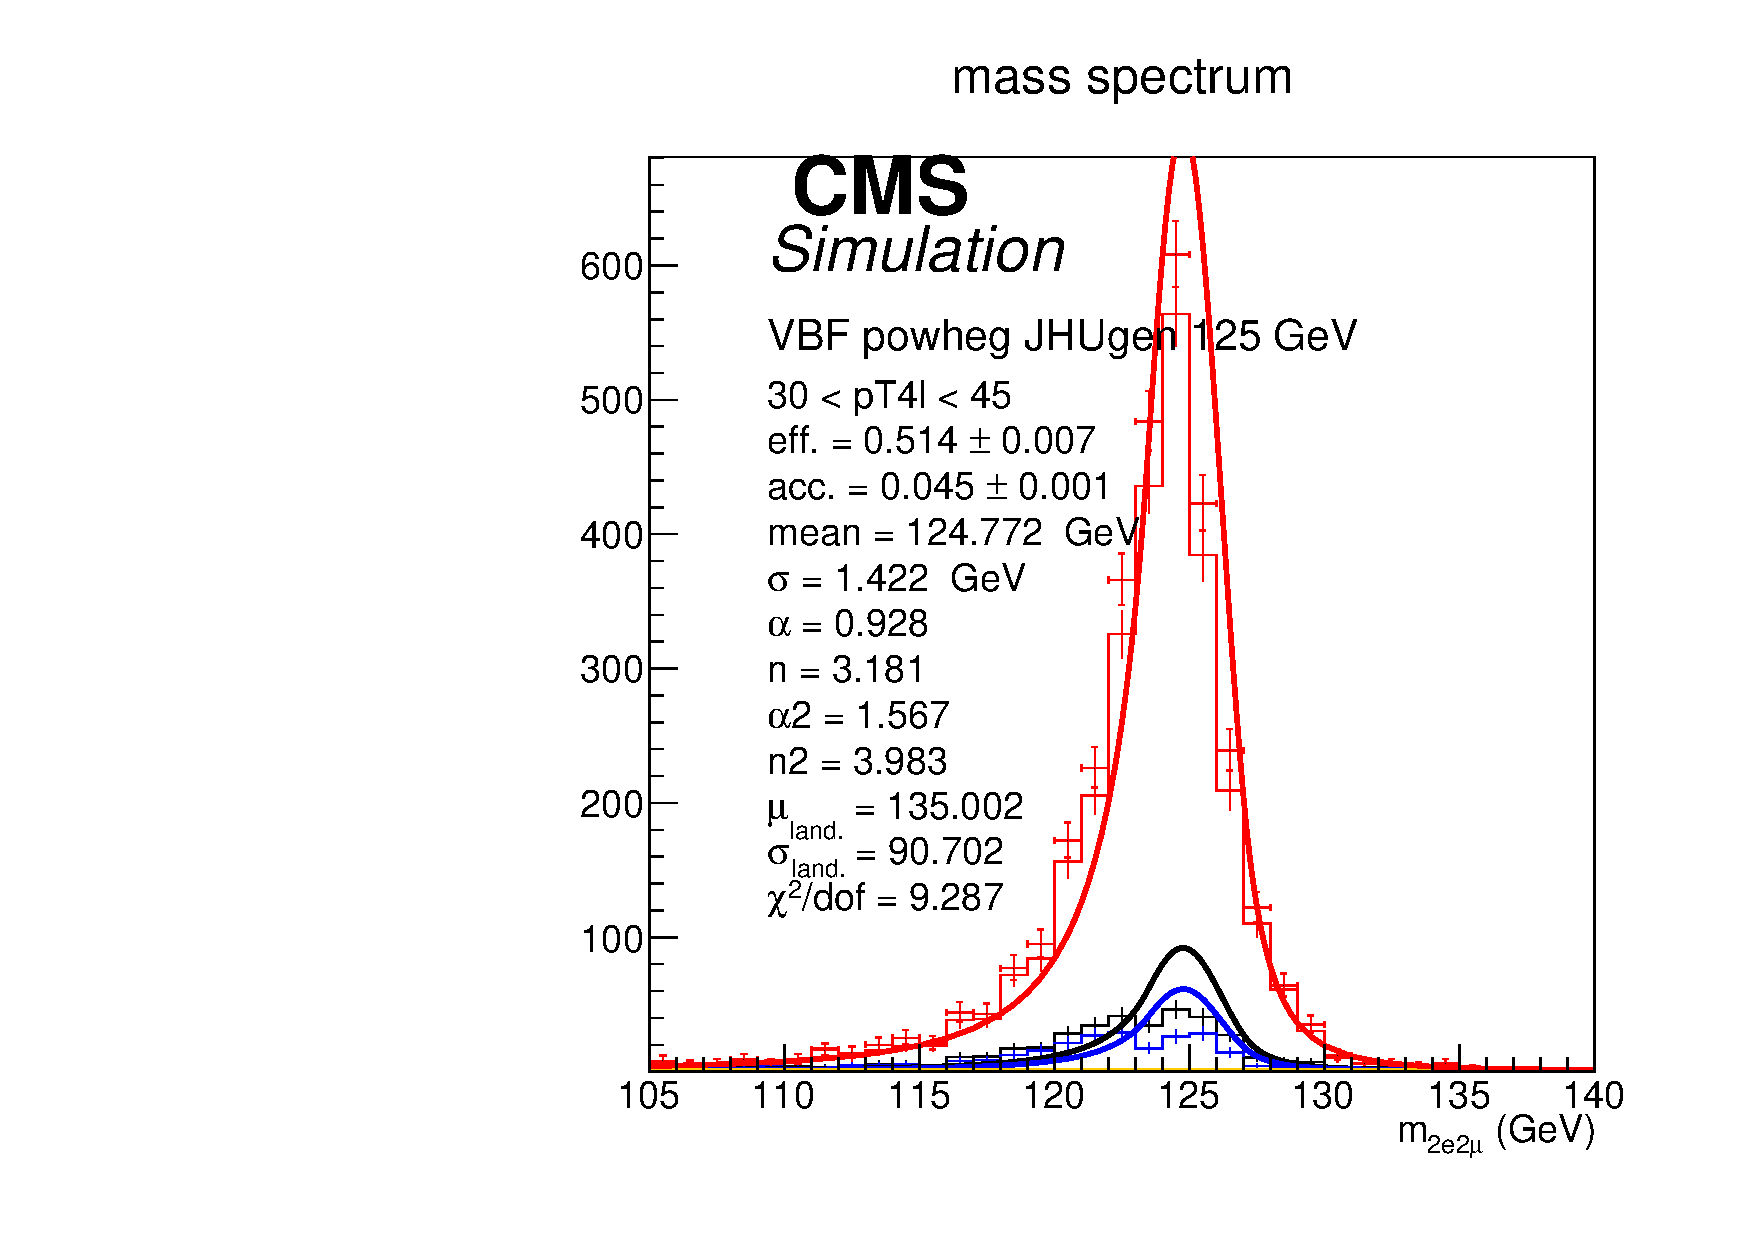
\includegraphics[width=0.3\textwidth,angle=0]{Figures/Appendix//VBF_powheg_JHUgen_125_2e2mu_pT4l_genbin2_recobin2_effs_genWeight*pileupWeight*dataMCWeight.pdf}
      \label{fig:sigfits-pT4l-VBF-powheg15-JHUgen-125-maintext:c}
    }  \\
    \subfigure[$45.0 < \pt(\mathrm{H}) < 80.0$]{
      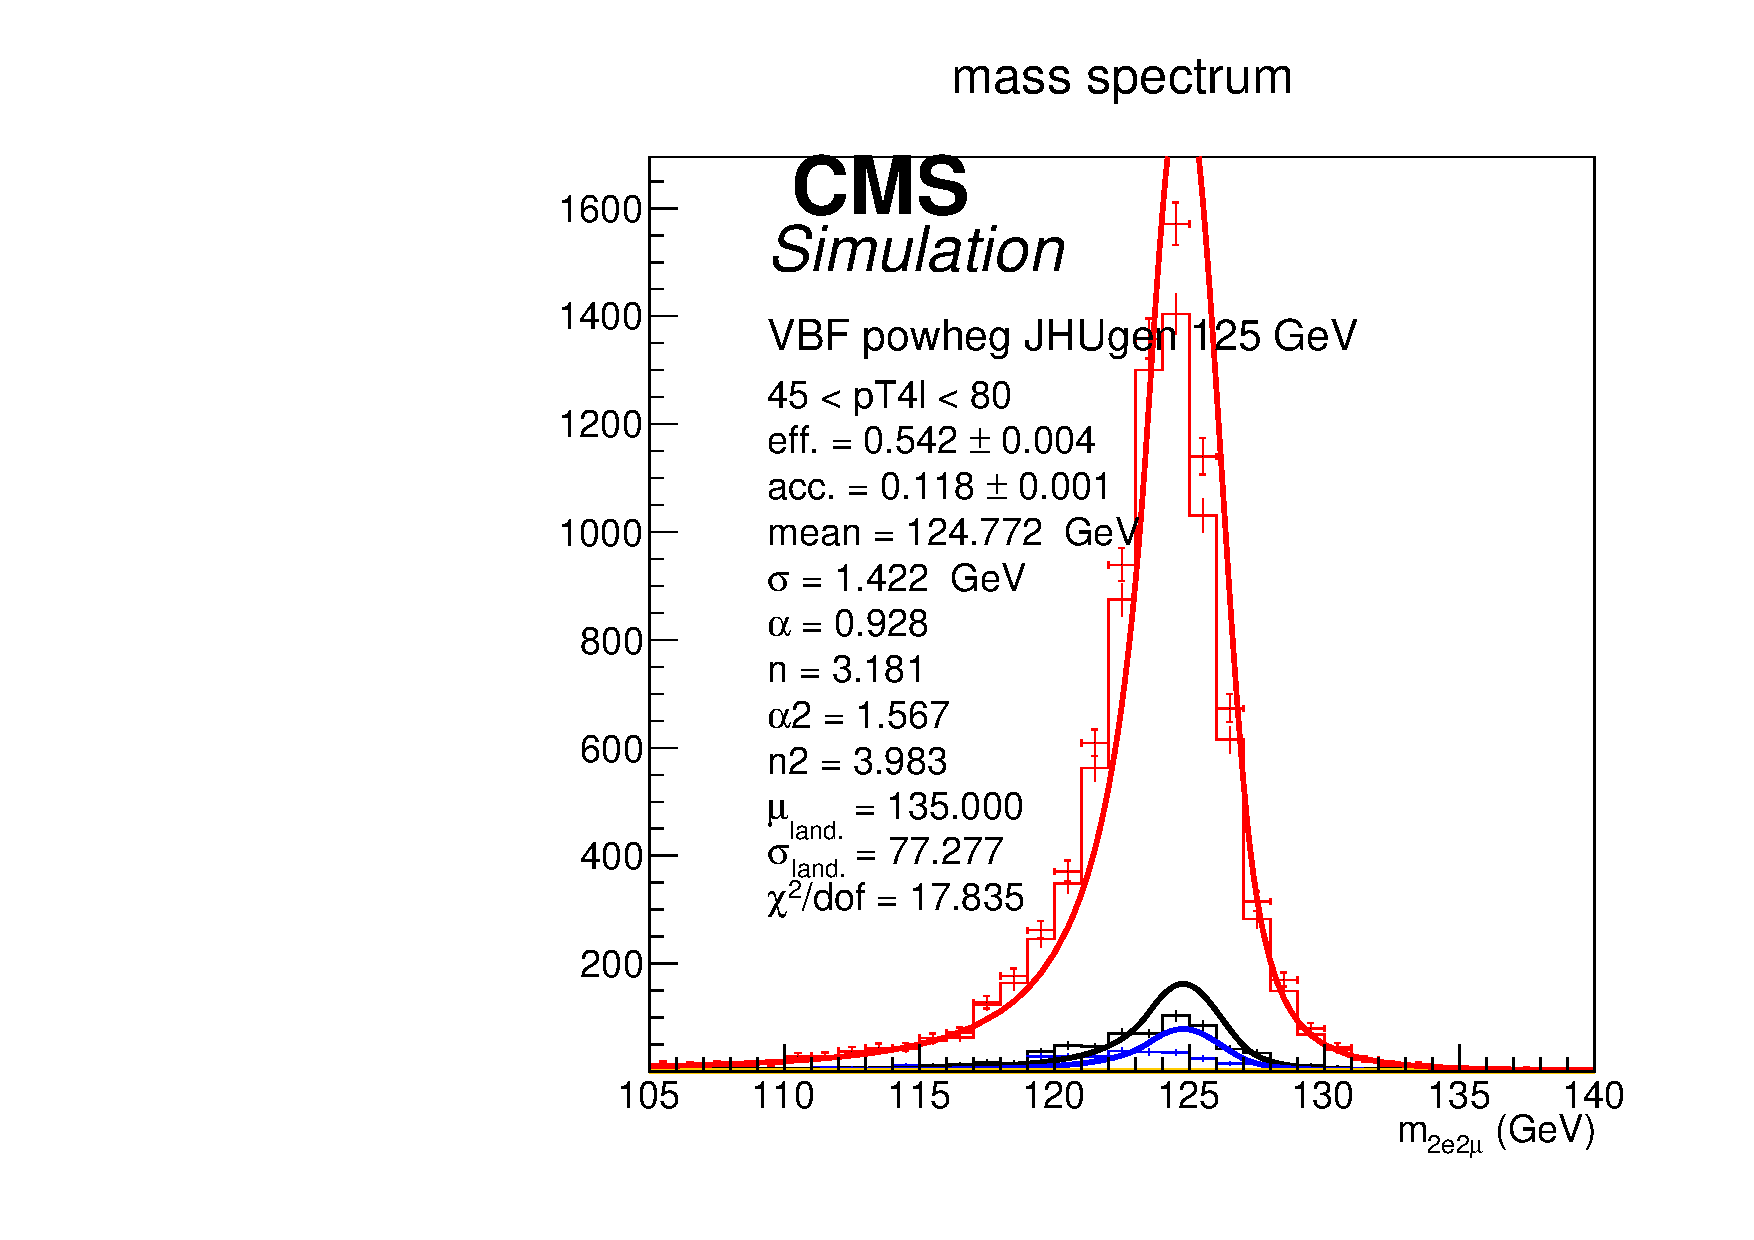
\includegraphics[width=0.3\textwidth,angle=0]{Figures/Appendix//VBF_powheg_JHUgen_125_2e2mu_pT4l_genbin3_recobin3_effs_genWeight*pileupWeight*dataMCWeight.pdf}
      \label{fig:sigfits-pT4l-VBF-powheg15-JHUgen-125-maintext:d}
    }
    \subfigure[$80.0 < \pt(\mathrm{H}) < 120.0$]{
      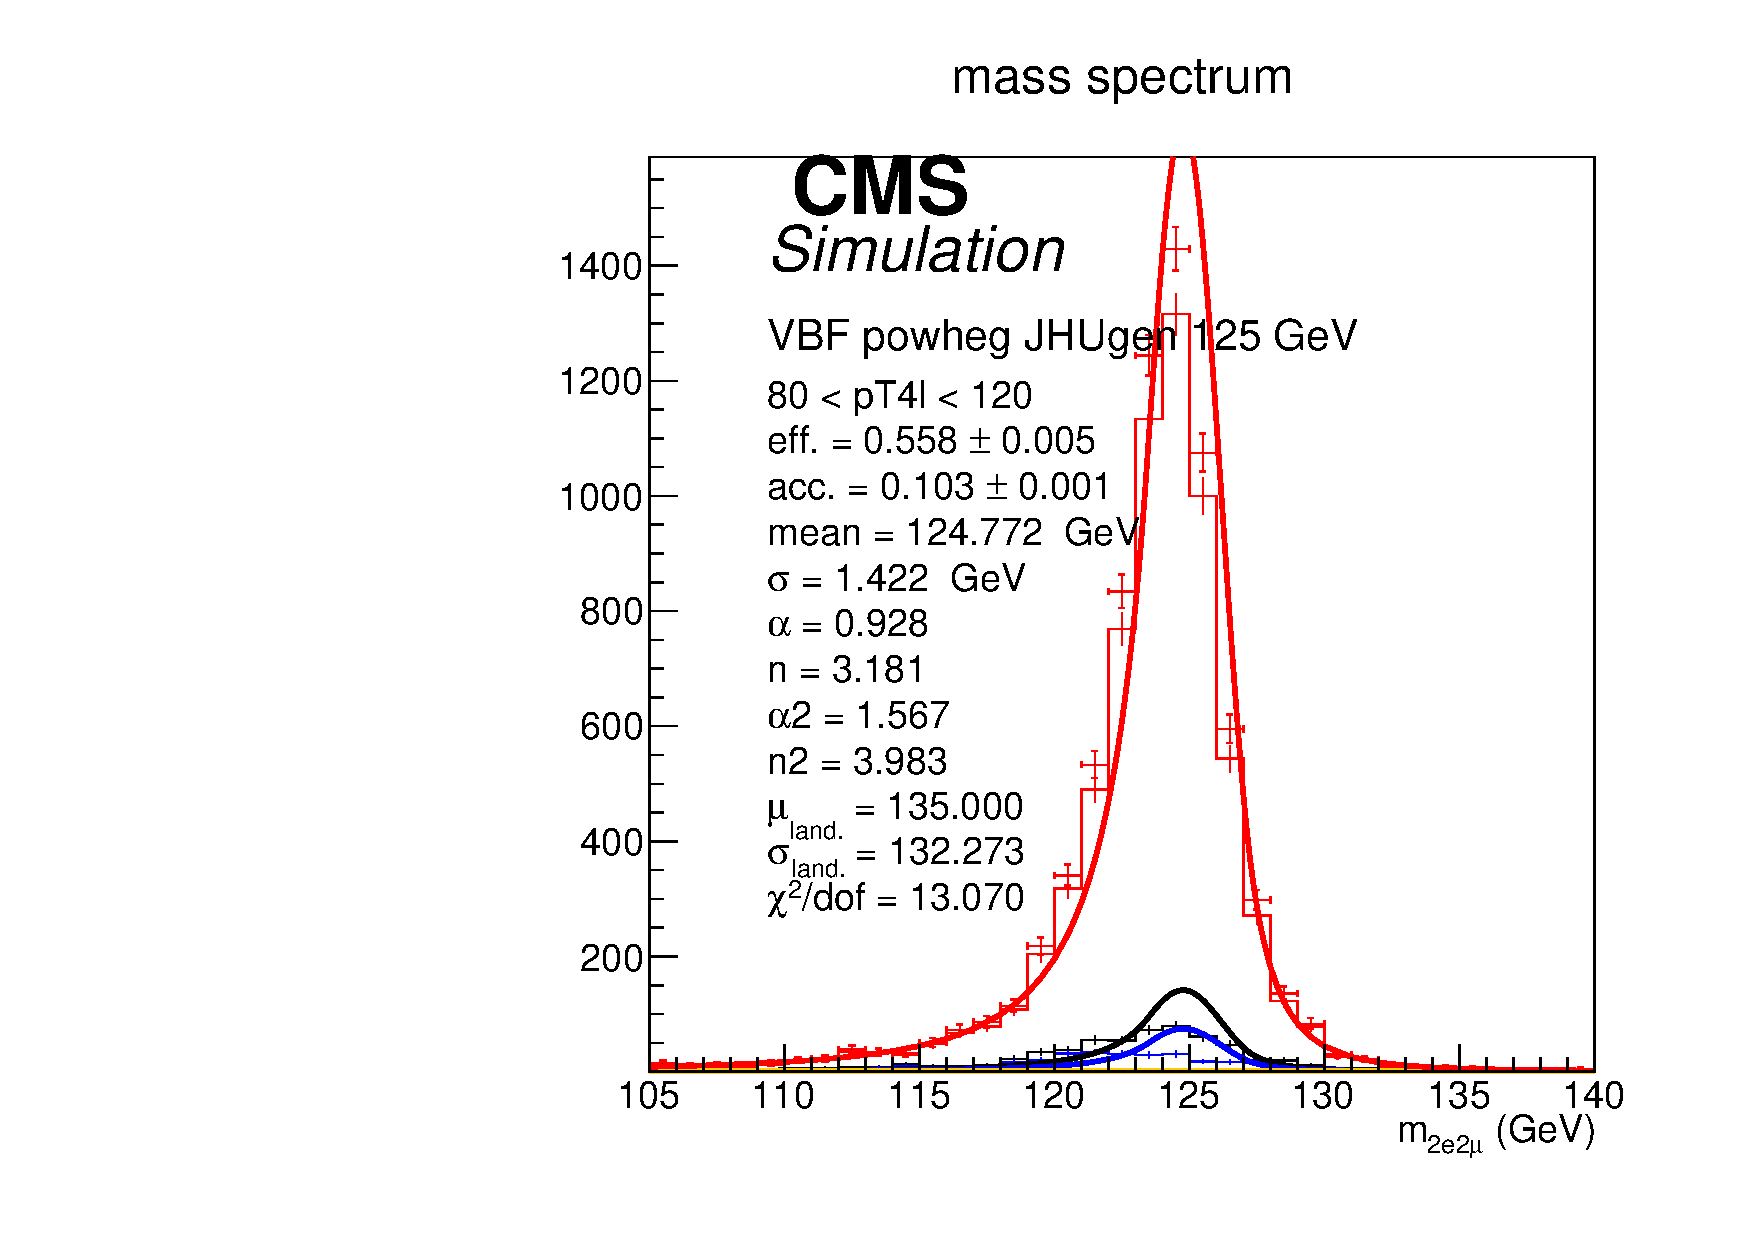
\includegraphics[width=0.3\textwidth,angle=0]{Figures/Appendix//VBF_powheg_JHUgen_125_2e2mu_pT4l_genbin4_recobin4_effs_genWeight*pileupWeight*dataMCWeight.pdf}
      \label{fig:sigfits-pT4l-VBF-powheg15-JHUgen-125-maintext:e}
    }
    \subfigure[$120.0 < \pt(\mathrm{H}) < 200.0$]{
      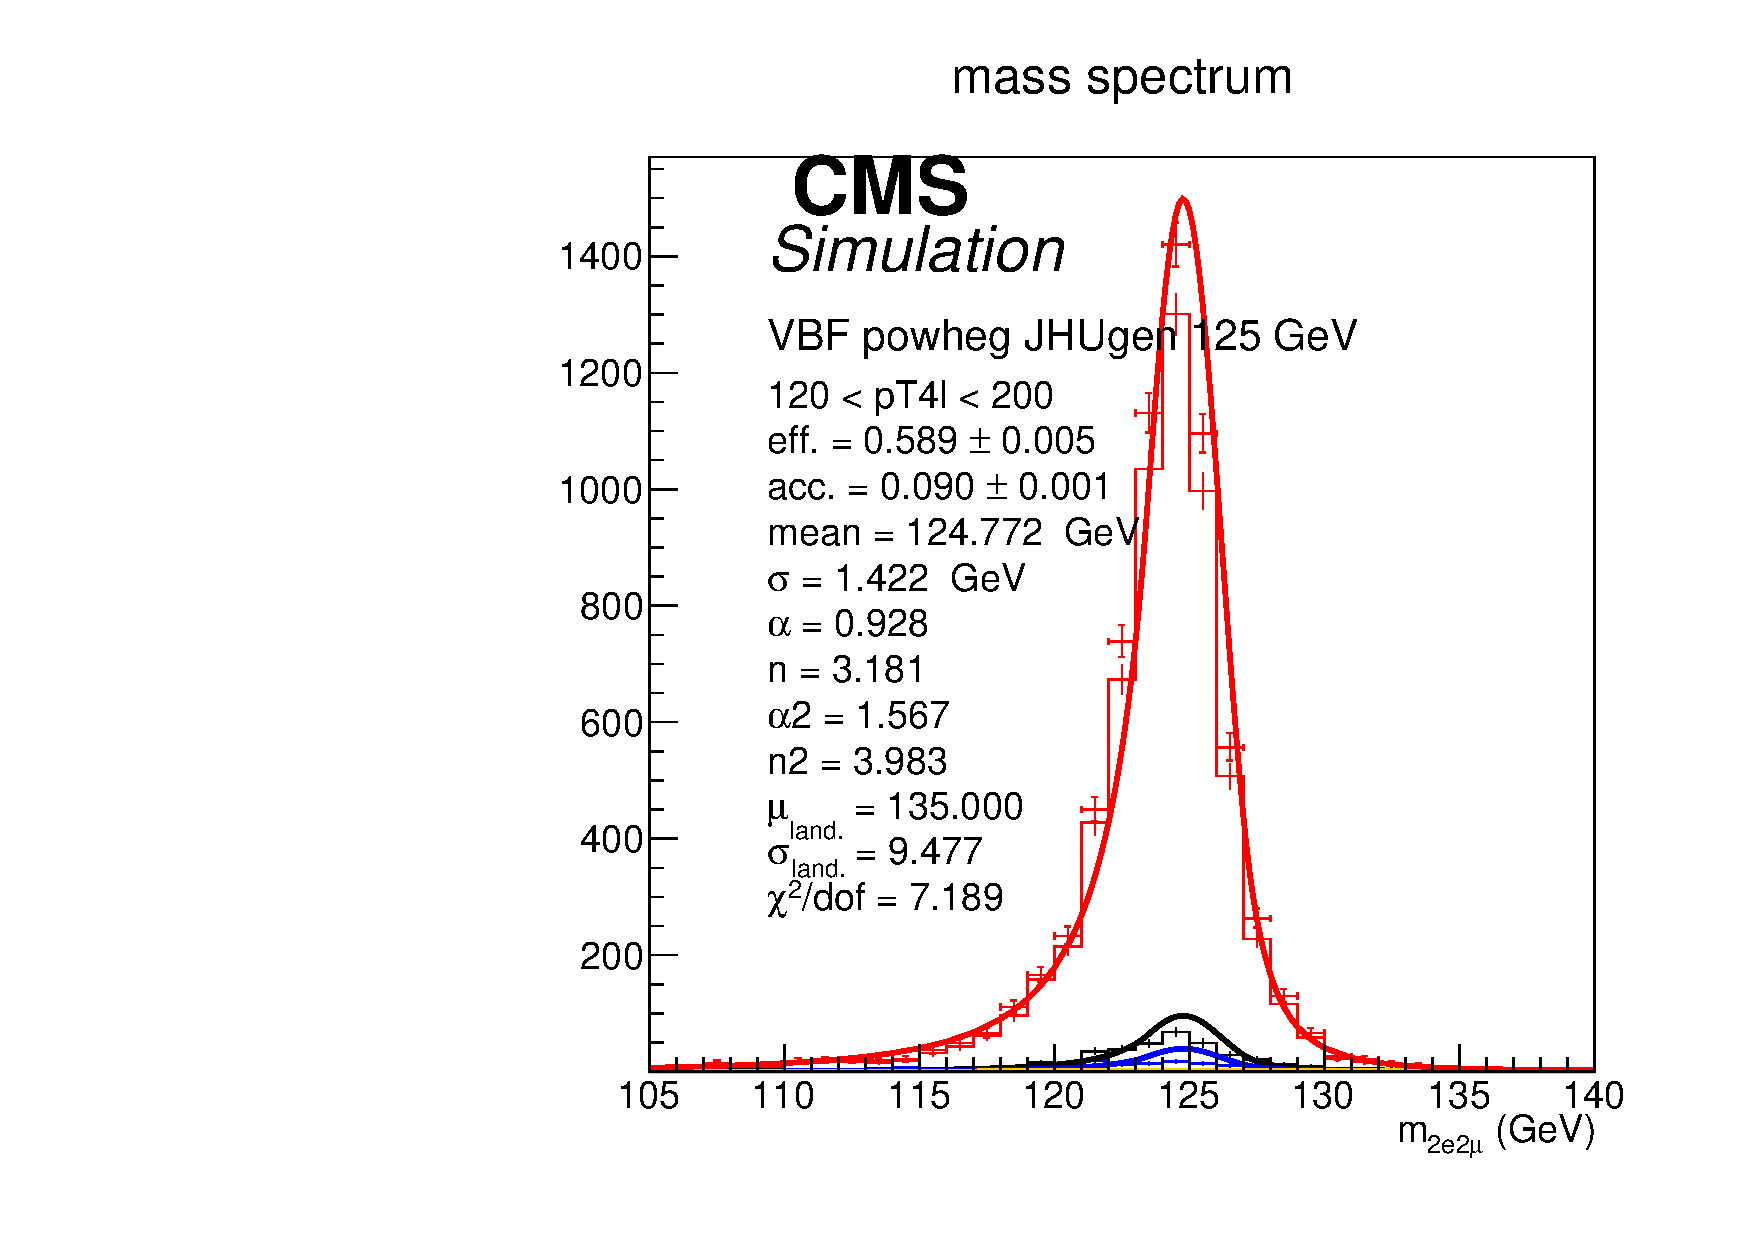
\includegraphics[width=0.3\textwidth,angle=0]{Figures/Appendix//VBF_powheg_JHUgen_125_2e2mu_pT4l_genbin5_recobin5_effs_genWeight*pileupWeight*dataMCWeight.pdf}
      \label{fig:sigfits-pT4l-VBF-powheg15-JHUgen-125-maintext:f}
    } \\
    \subfigure[$200.0 < \pt(\mathrm{H}) < 13000.0$]{
      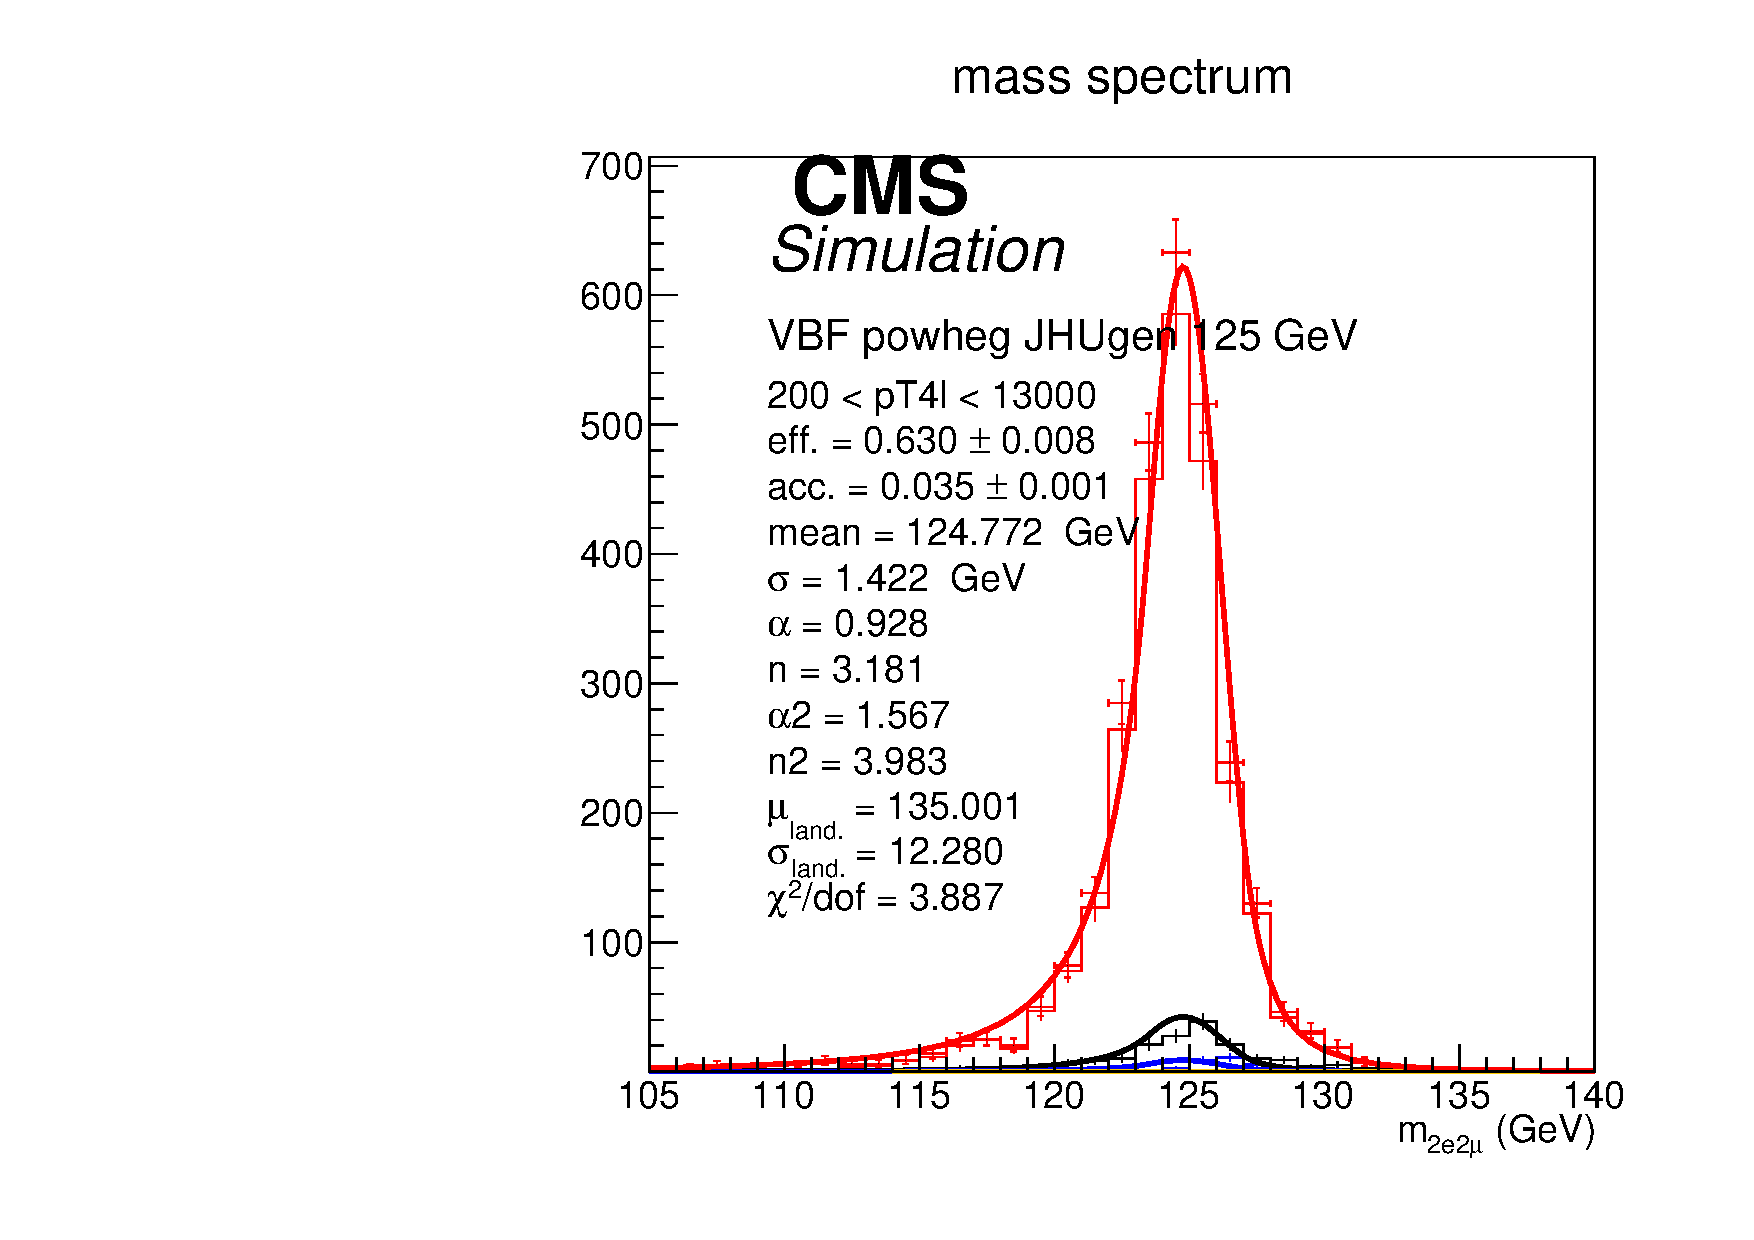
\includegraphics[width=0.3\textwidth,angle=0]{Figures/Appendix//VBF_powheg_JHUgen_125_2e2mu_pT4l_genbin6_recobin6_effs_genWeight*pileupWeight*dataMCWeight.pdf}
      \label{fig:sigfits-pT4l-VBF-powheg15-JHUgen-125-maintext:g}
    }
    \\
    \caption{ Example signal shapes at reconstruction level for a resonance of m(4$\ell$) in $2e2\mu$ final state for the $VBF$ production mode from {\sc powheg+JHUGen} in different bins of $\pt(\mathrm{H})$. The black curve represents events which do not pass the fiducial volume selection. The curve has no effect on the result.
    }
  \label{fig:sigfits-pT4l-VBF-powheg15-JHUgen-125-maintext}
 \end{center}
\end{figure} \clearpage

\begin{figure}[htb]
  \begin{center}
    \subfigure[$0.0 < \pt(\mathrm{H}) < 15.0 $]{
      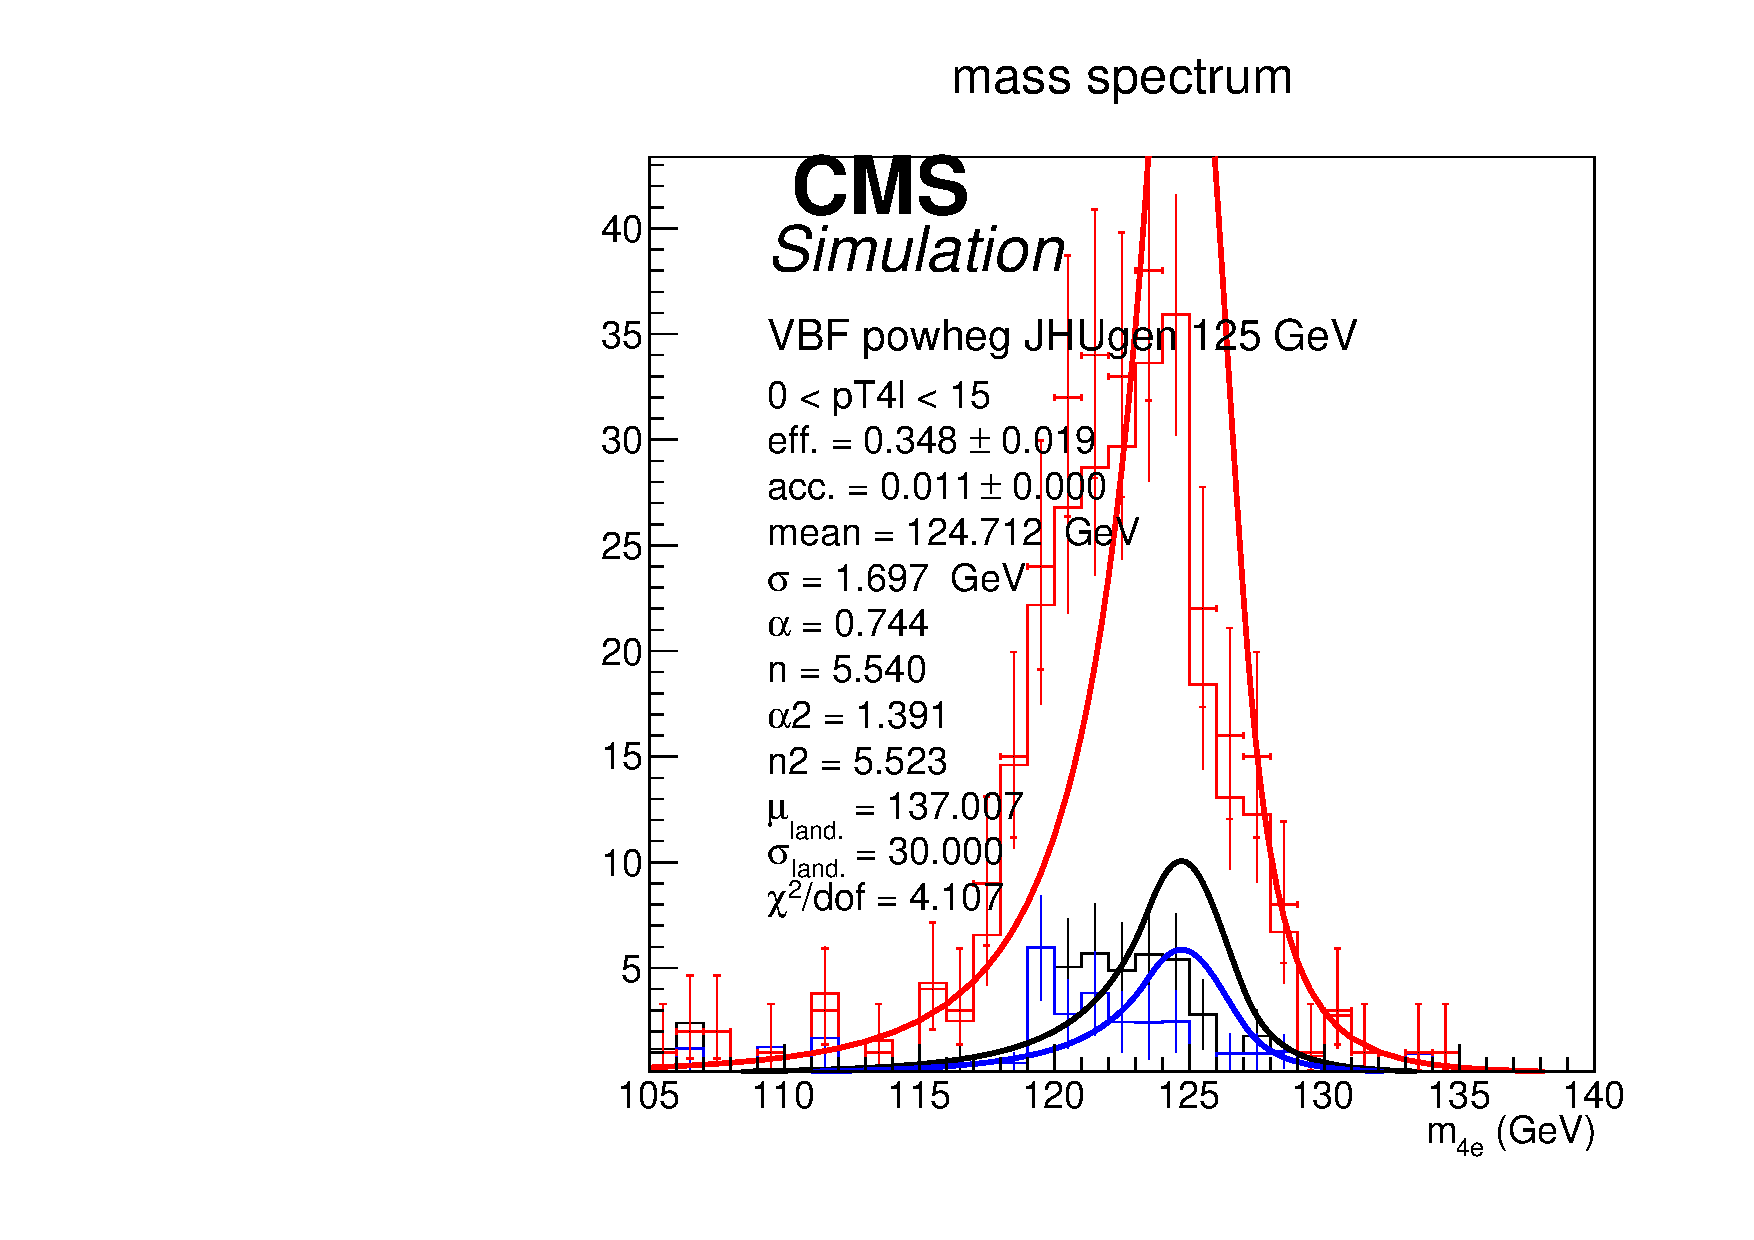
\includegraphics[width=0.3\textwidth,angle=0]{Figures/Appendix//VBF_powheg_JHUgen_125_4e_pT4l_genbin0_recobin0_effs_genWeight*pileupWeight*dataMCWeight.pdf}
      \label{fig:sigfits-pT4l-VBF-powheg15-JHUgen-125-maintext:a}
    }
    \subfigure[$15.0 < \pt(\mathrm{H}) < 30.0$]{
      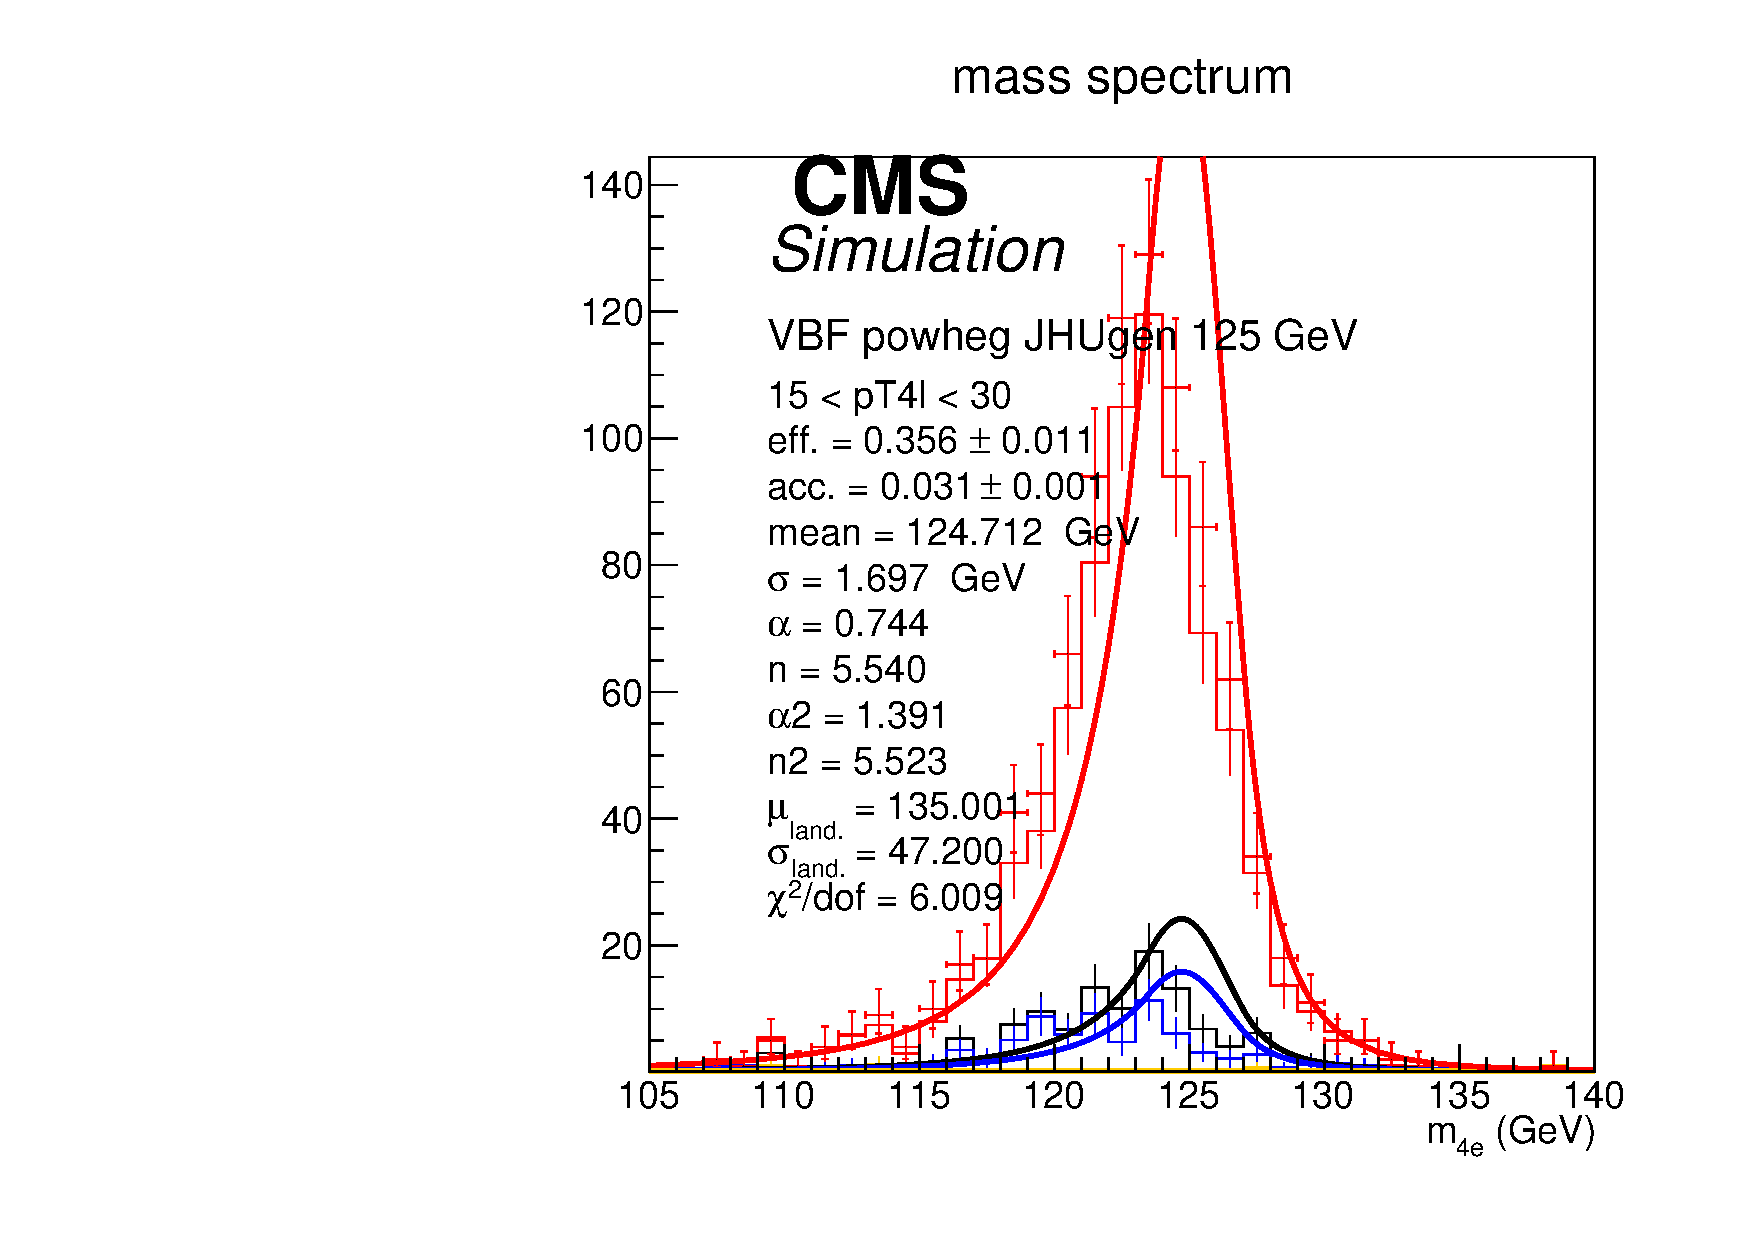
\includegraphics[width=0.3\textwidth,angle=0]{Figures/Appendix//VBF_powheg_JHUgen_125_4e_pT4l_genbin1_recobin1_effs_genWeight*pileupWeight*dataMCWeight.pdf}
      \label{fig:sigfits-pT4l-VBF-powheg15-JHUgen-125-maintext:b}
    }
   \subfigure[$30.0 < \pt(\mathrm{H}) < 45.0$]{
      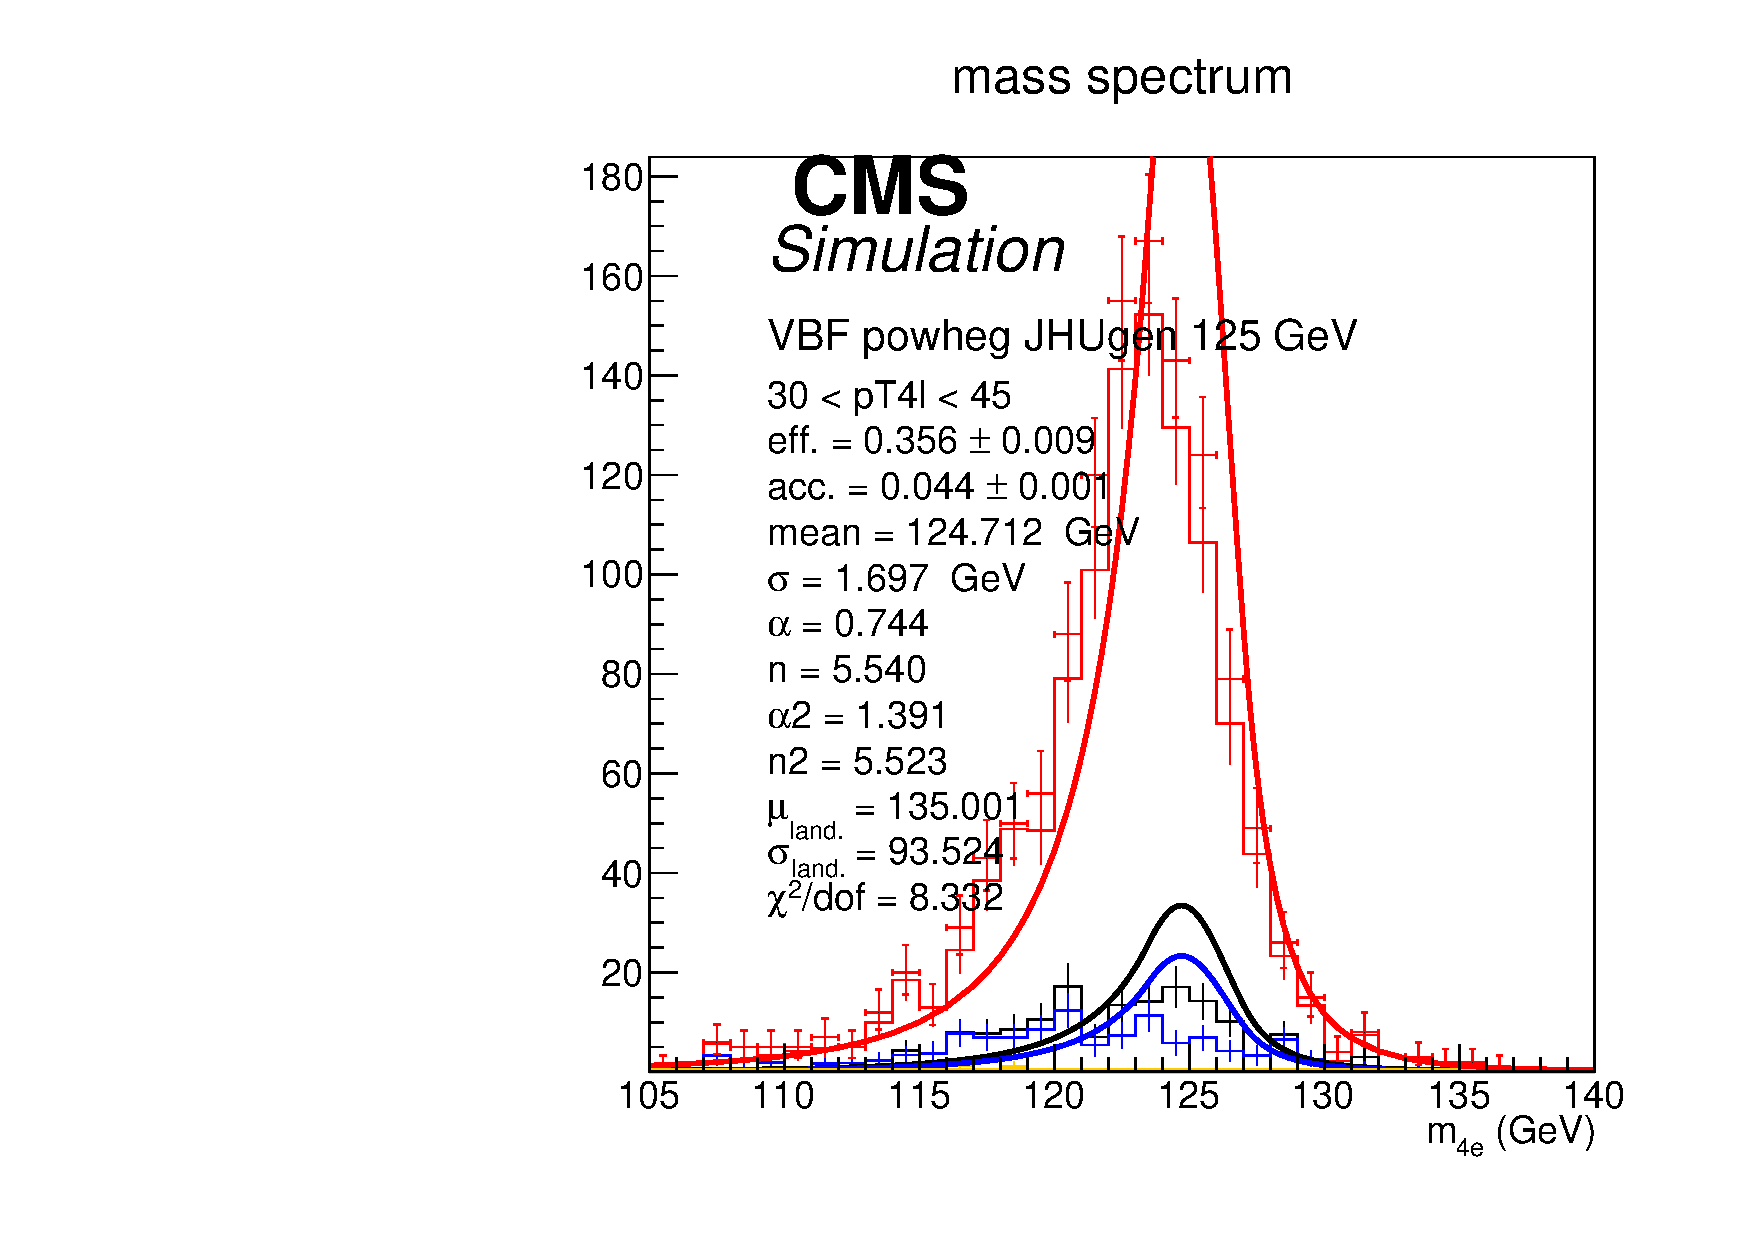
\includegraphics[width=0.3\textwidth,angle=0]{Figures/Appendix//VBF_powheg_JHUgen_125_4e_pT4l_genbin2_recobin2_effs_genWeight*pileupWeight*dataMCWeight.pdf}
      \label{fig:sigfits-pT4l-VBF-powheg15-JHUgen-125-maintext:c}
    }  \\
    \subfigure[$45.0 < \pt(\mathrm{H}) < 80.0$]{
      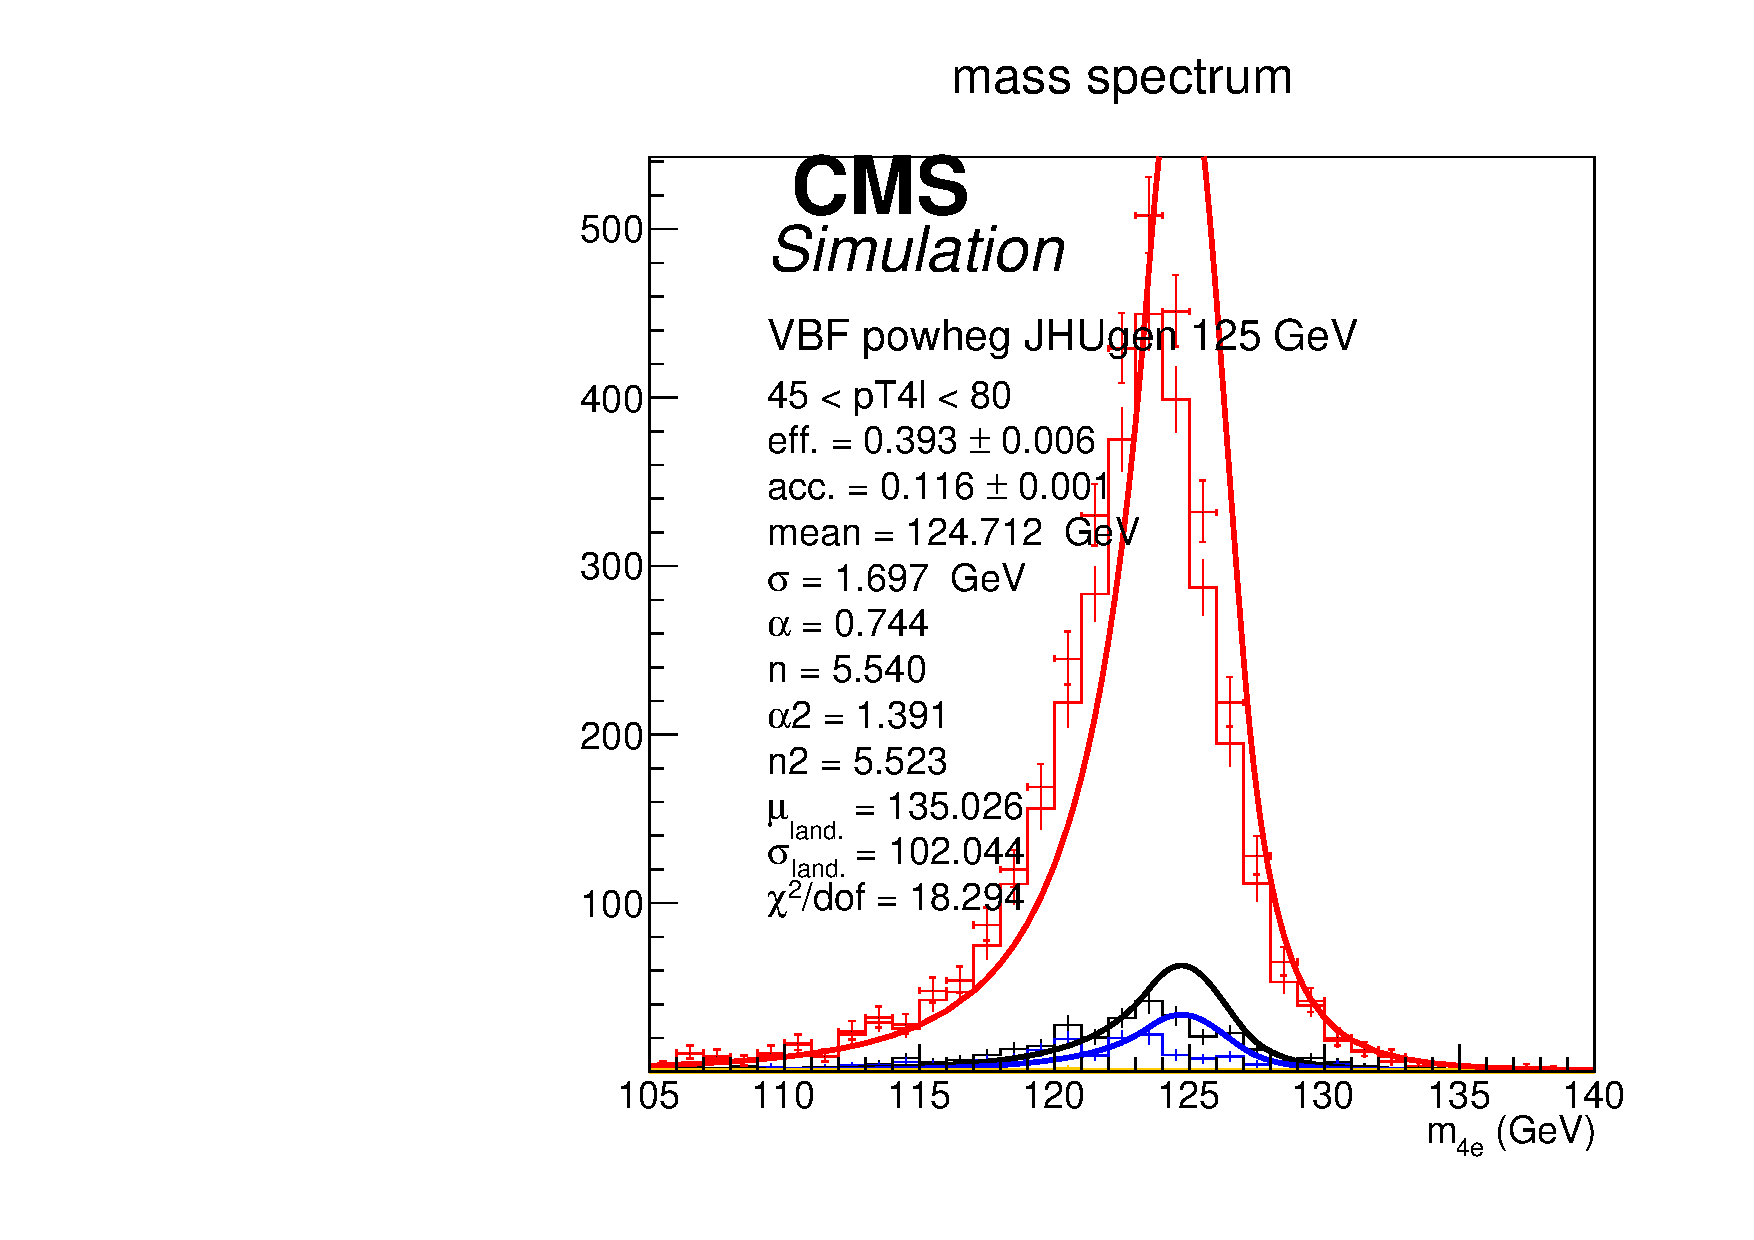
\includegraphics[width=0.3\textwidth,angle=0]{Figures/Appendix//VBF_powheg_JHUgen_125_4e_pT4l_genbin3_recobin3_effs_genWeight*pileupWeight*dataMCWeight.pdf}
      \label{fig:sigfits-pT4l-VBF-powheg15-JHUgen-125-maintext:d}
    }
    \subfigure[$80.0 < \pt(\mathrm{H}) < 120.0$]{
      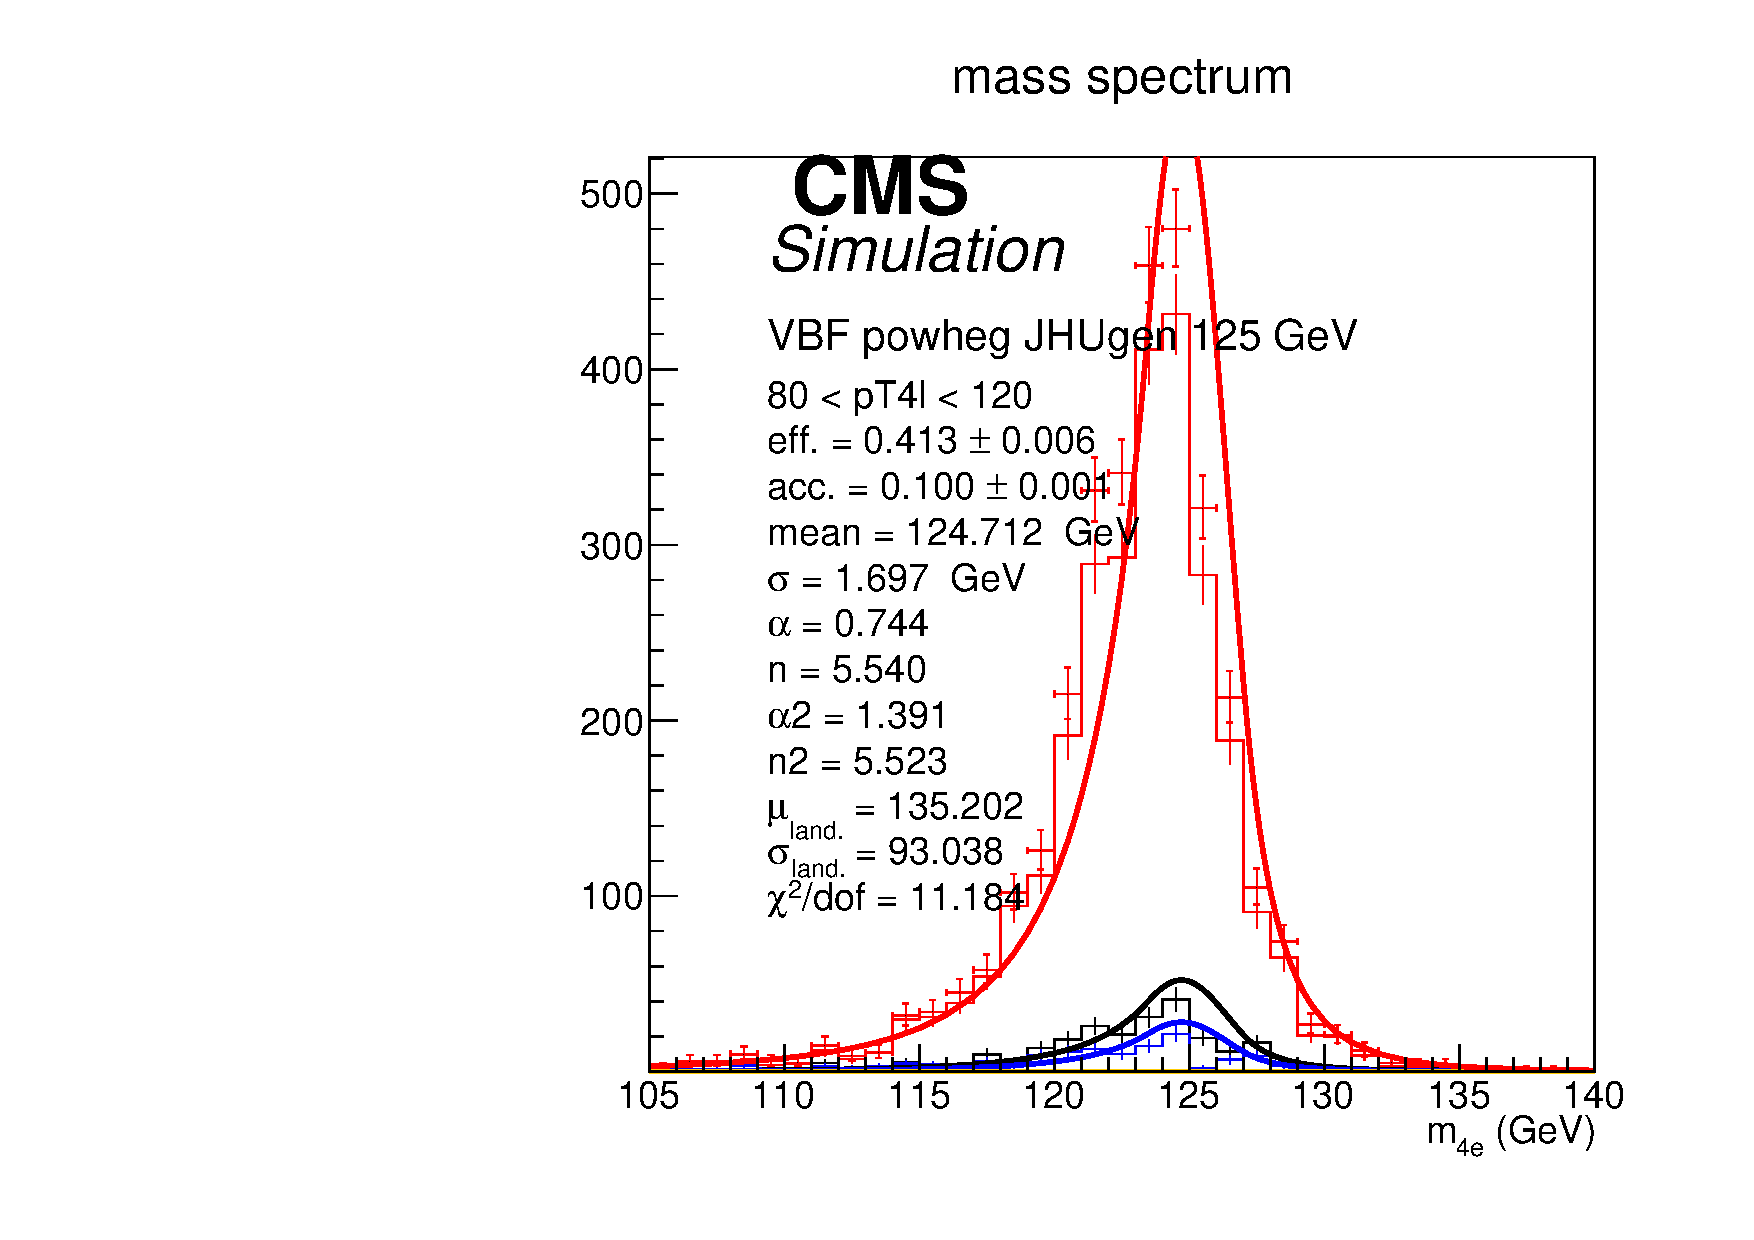
\includegraphics[width=0.3\textwidth,angle=0]{Figures/Appendix//VBF_powheg_JHUgen_125_4e_pT4l_genbin4_recobin4_effs_genWeight*pileupWeight*dataMCWeight.pdf}
      \label{fig:sigfits-pT4l-VBF-powheg15-JHUgen-125-maintext:e}
    }
    \subfigure[$120.0 < \pt(\mathrm{H}) < 200.0$]{
      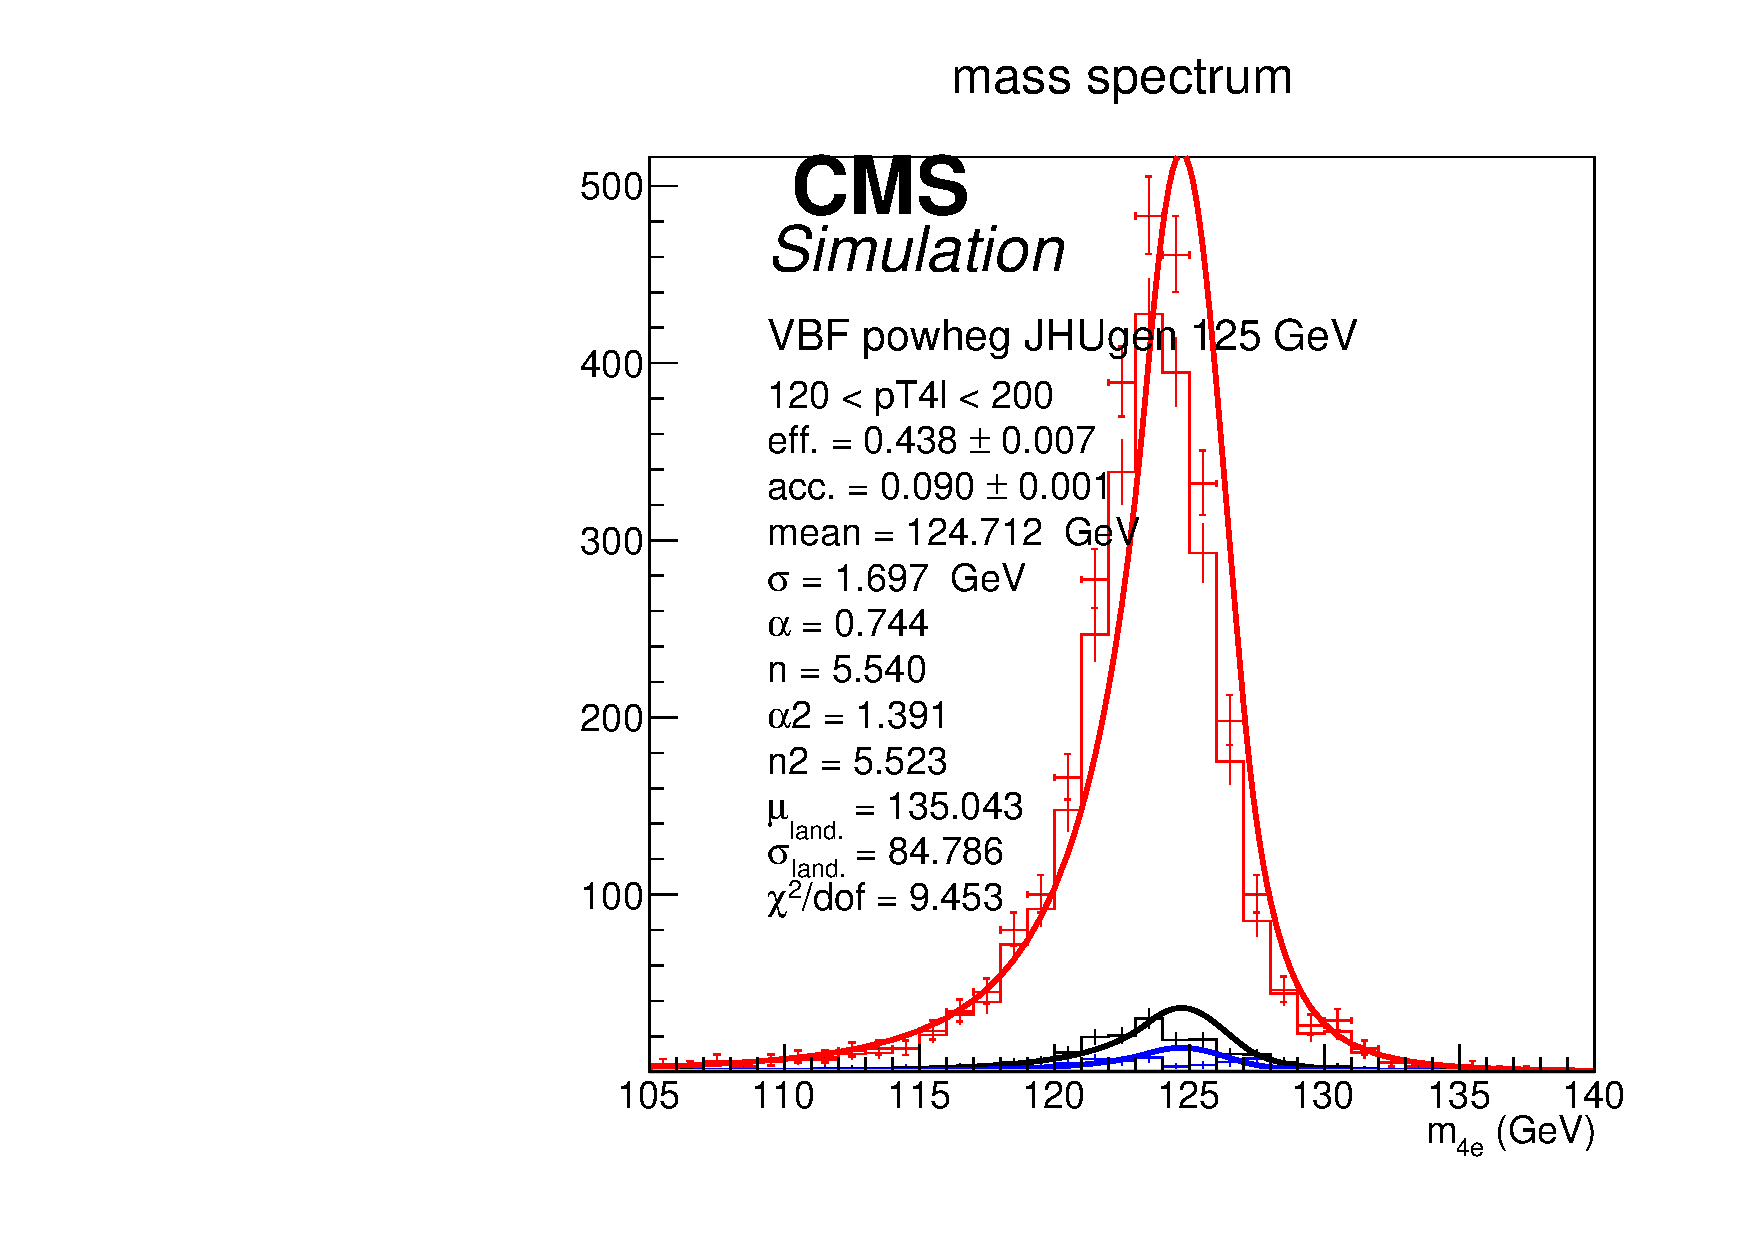
\includegraphics[width=0.3\textwidth,angle=0]{Figures/Appendix//VBF_powheg_JHUgen_125_4e_pT4l_genbin5_recobin5_effs_genWeight*pileupWeight*dataMCWeight.pdf}
      \label{fig:sigfits-pT4l-VBF-powheg15-JHUgen-125-maintext:f}
    } \\
    \subfigure[$200.0 < \pt(\mathrm{H}) < 13000.0$]{
      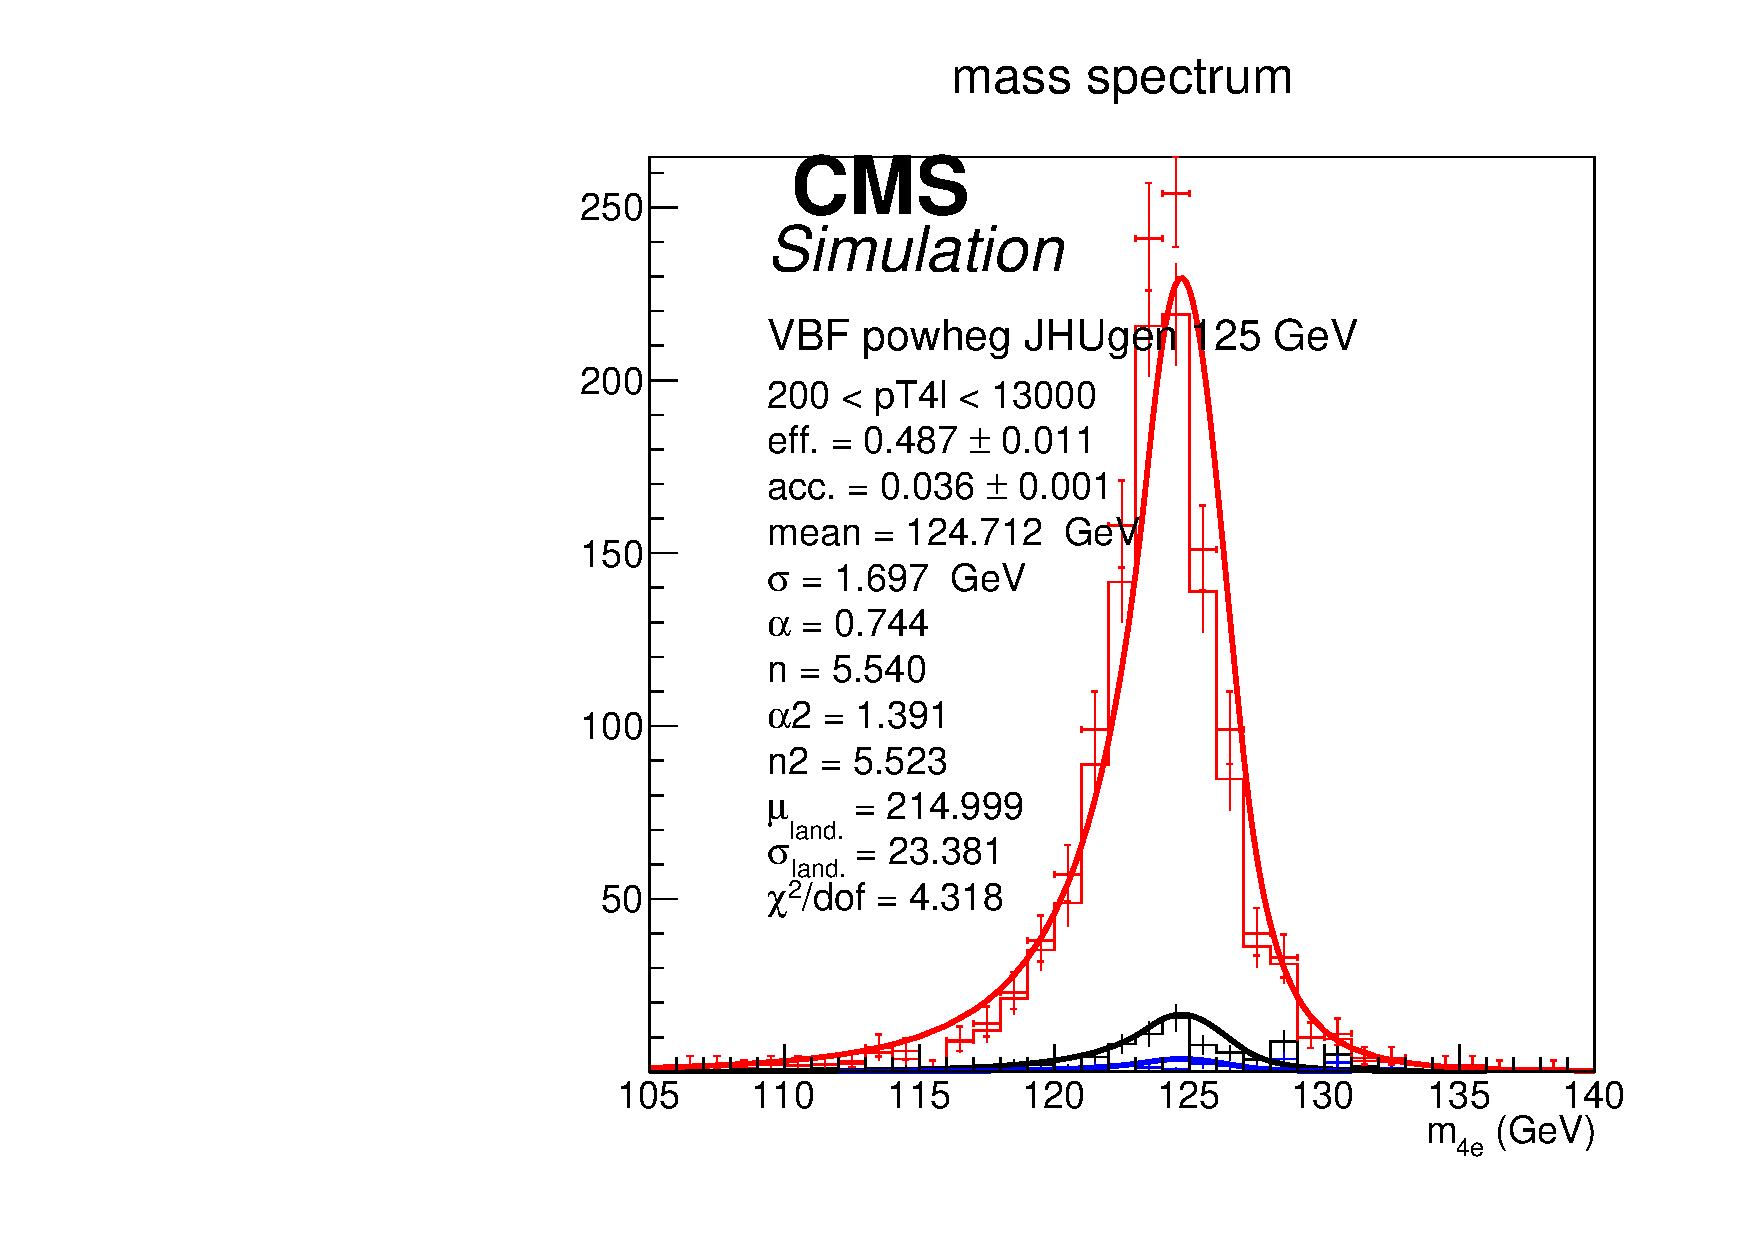
\includegraphics[width=0.3\textwidth,angle=0]{Figures/Appendix//VBF_powheg_JHUgen_125_4e_pT4l_genbin6_recobin6_effs_genWeight*pileupWeight*dataMCWeight.pdf}
      \label{fig:sigfits-pT4l-VBF-powheg15-JHUgen-125-maintext:g}
    }
    \\
    \caption{ Example signal shapes at reconstruction level for a resonance of m(4$\ell$) in $4e$ final state for the $VBF$ production mode from {\sc powheg+JHUGen} in different bins of $\pt(\mathrm{H})$. The black curve represents events which do not pass the fiducial volume selection. The curve has no effect on the result.
    }
  \label{fig:sigfits-pT4l-VBF-powheg15-JHUgen-125-maintext}
 \end{center}
\end{figure} \clearpage


\begin{figure}[htb]
  \begin{center}
    \subfigure[$0.0 < \pt(\mathrm{H}) < 15.0 $]{
      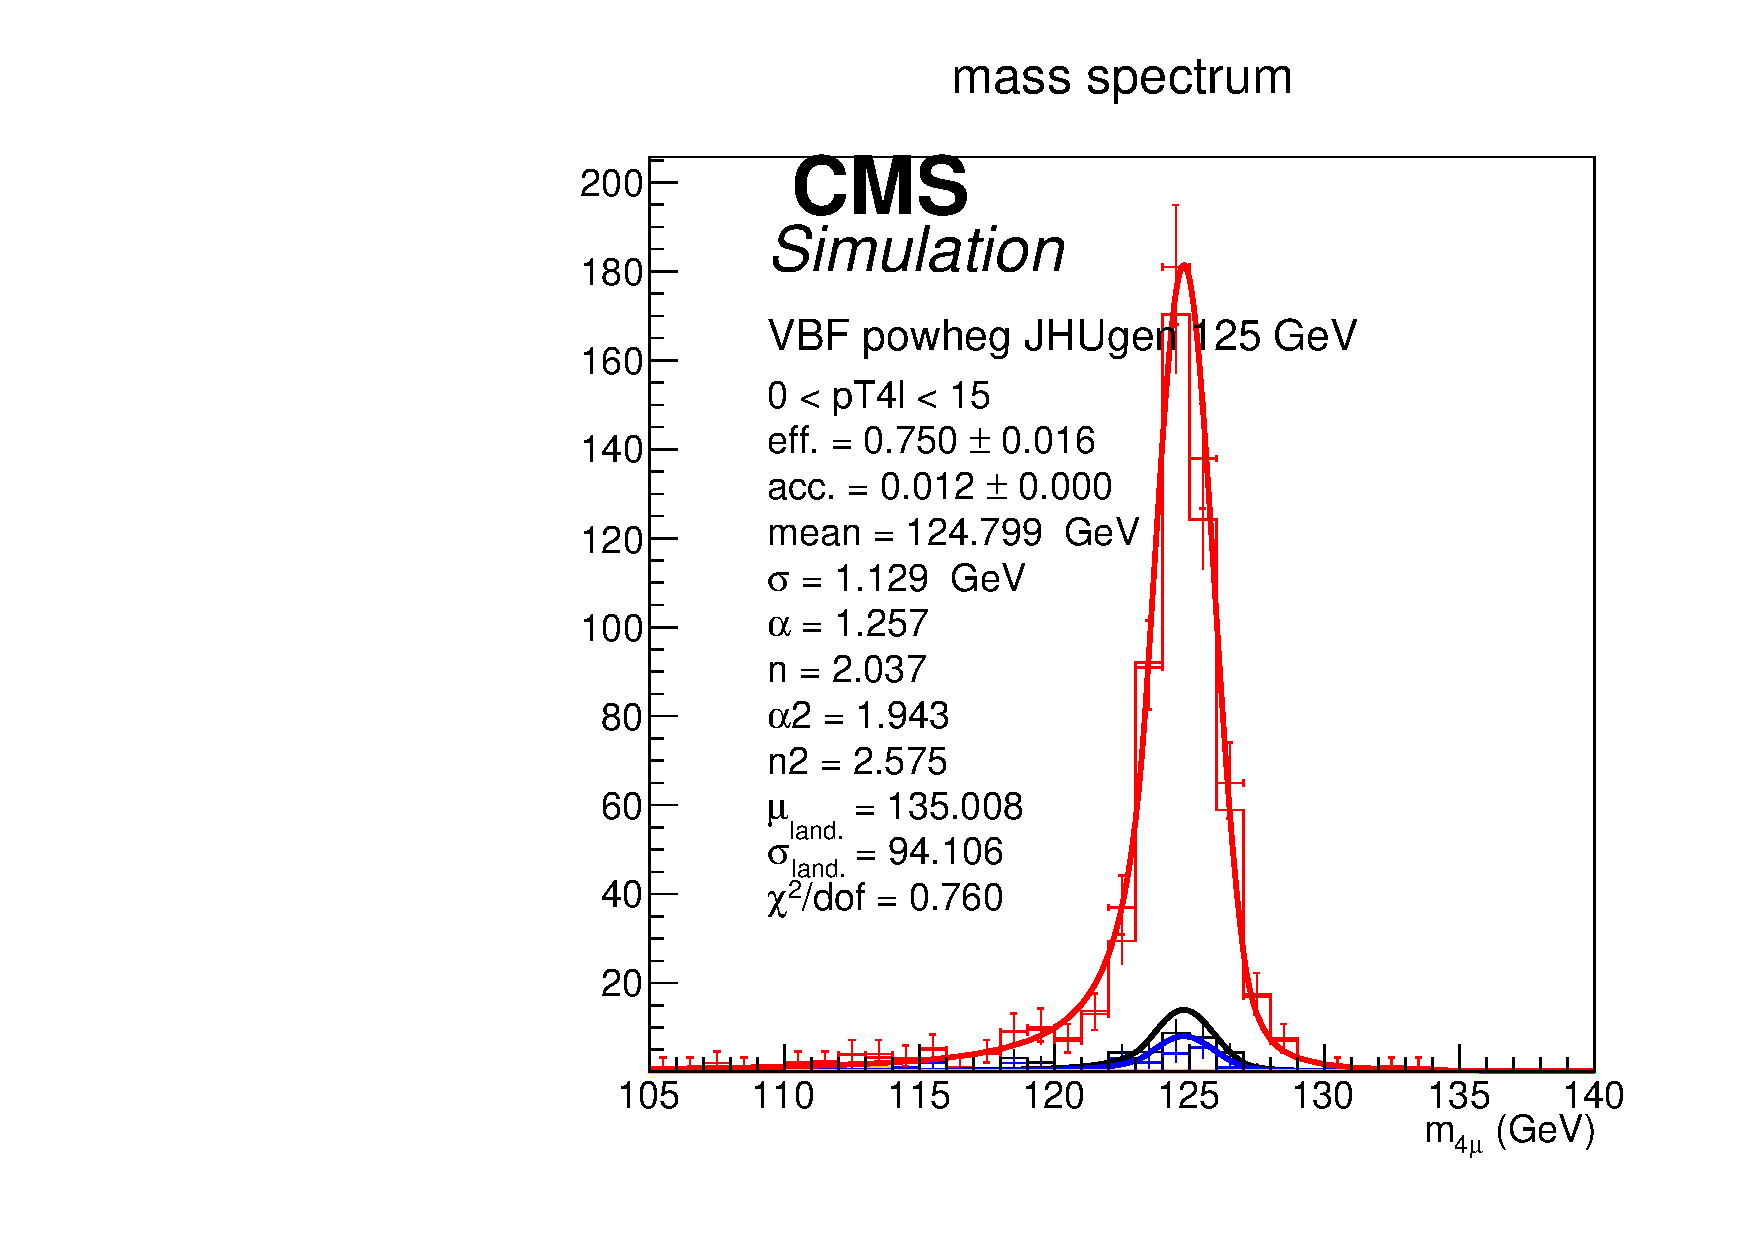
\includegraphics[width=0.3\textwidth,angle=0]{Figures/Appendix//VBF_powheg_JHUgen_125_4mu_pT4l_genbin0_recobin0_effs_genWeight*pileupWeight*dataMCWeight.pdf}
      \label{fig:sigfits-pT4l-VBF-powheg15-JHUgen-125-maintext:a}
    }
    \subfigure[$15.0 < \pt(\mathrm{H}) < 30.0$]{
      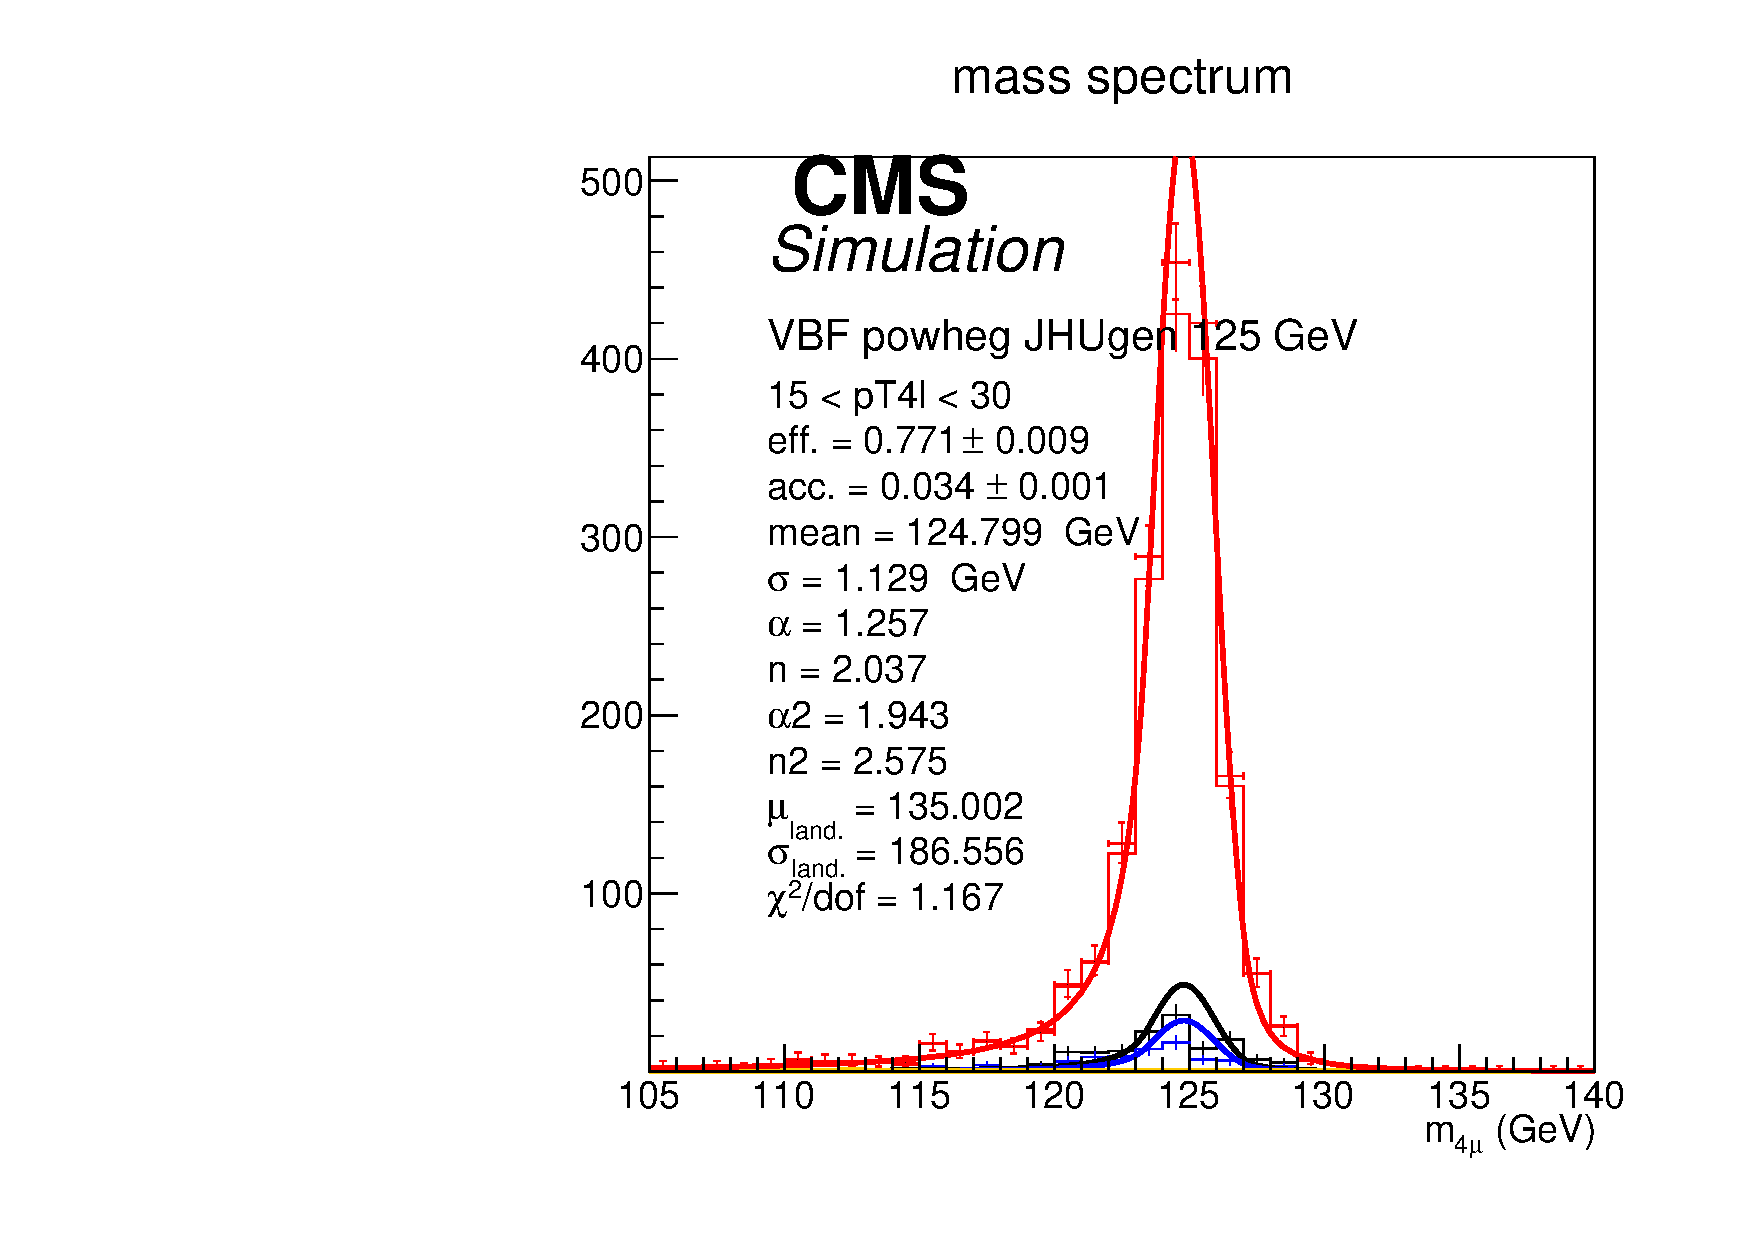
\includegraphics[width=0.3\textwidth,angle=0]{Figures/Appendix//VBF_powheg_JHUgen_125_4mu_pT4l_genbin1_recobin1_effs_genWeight*pileupWeight*dataMCWeight.pdf}
      \label{fig:sigfits-pT4l-VBF-powheg15-JHUgen-125-maintext:b}
    }
   \subfigure[$30.0 < \pt(\mathrm{H}) < 45.0$]{
      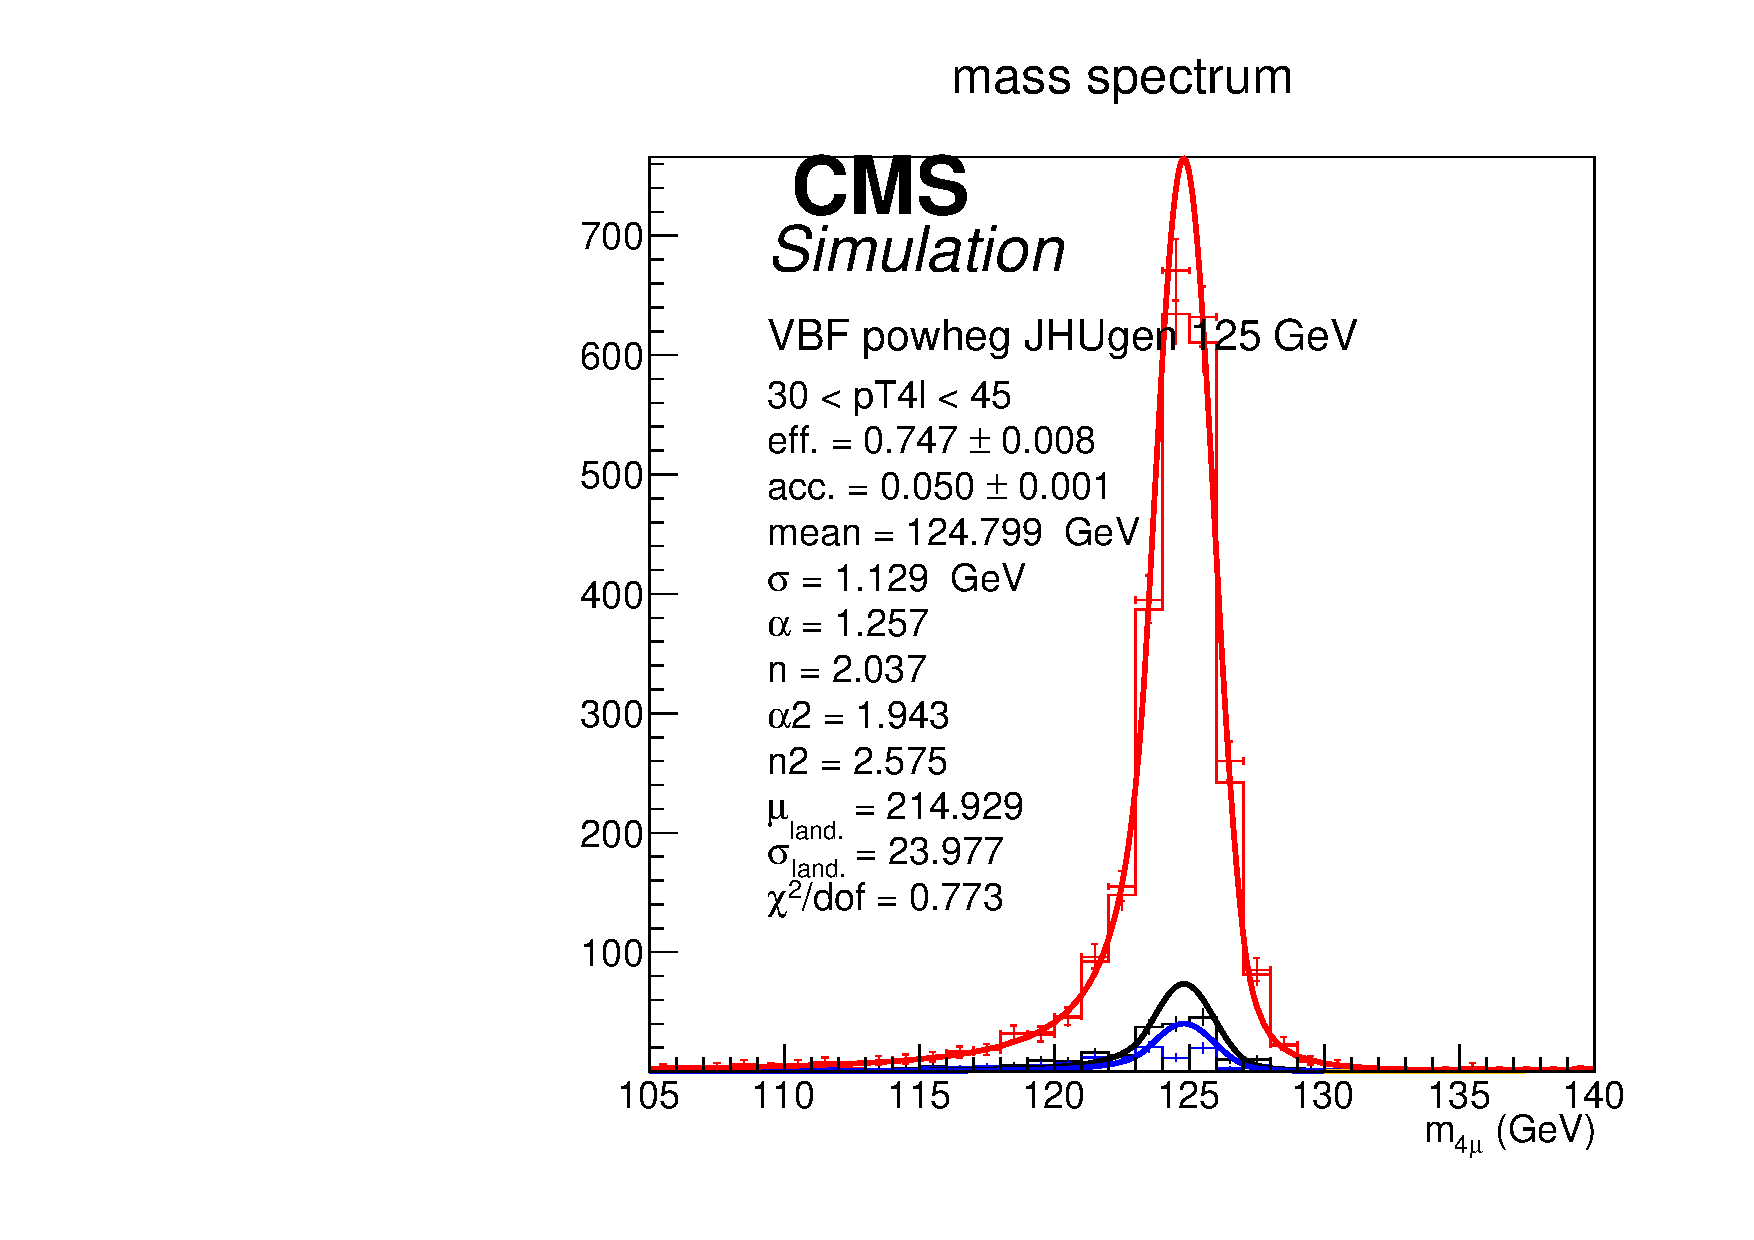
\includegraphics[width=0.3\textwidth,angle=0]{Figures/Appendix//VBF_powheg_JHUgen_125_4mu_pT4l_genbin2_recobin2_effs_genWeight*pileupWeight*dataMCWeight.pdf}
      \label{fig:sigfits-pT4l-VBF-powheg15-JHUgen-125-maintext:c}
    }  \\
    \subfigure[$45.0 < \pt(\mathrm{H}) < 80.0$]{
      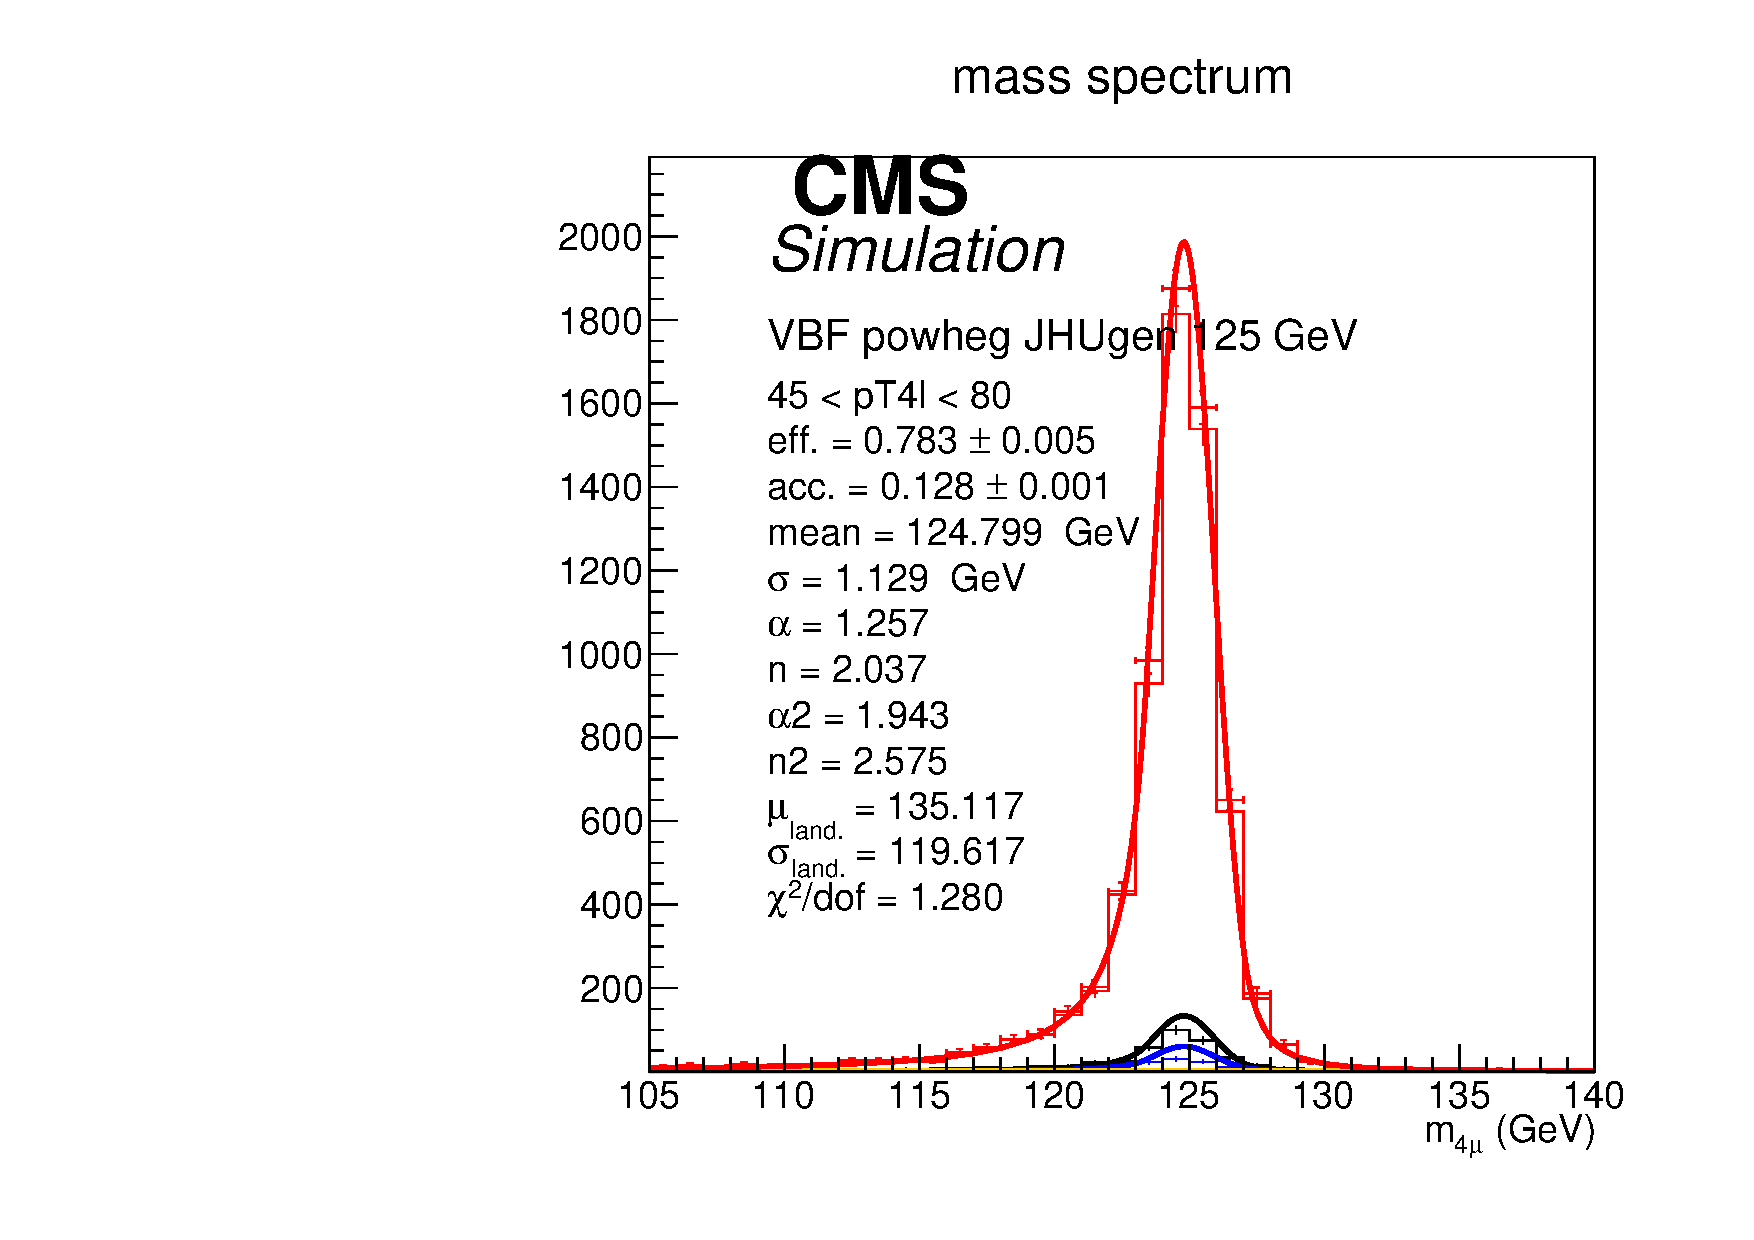
\includegraphics[width=0.3\textwidth,angle=0]{Figures/Appendix//VBF_powheg_JHUgen_125_4mu_pT4l_genbin3_recobin3_effs_genWeight*pileupWeight*dataMCWeight.pdf}
      \label{fig:sigfits-pT4l-VBF-powheg15-JHUgen-125-maintext:d}
    }
    \subfigure[$80.0 < \pt(\mathrm{H}) < 120.0$]{
      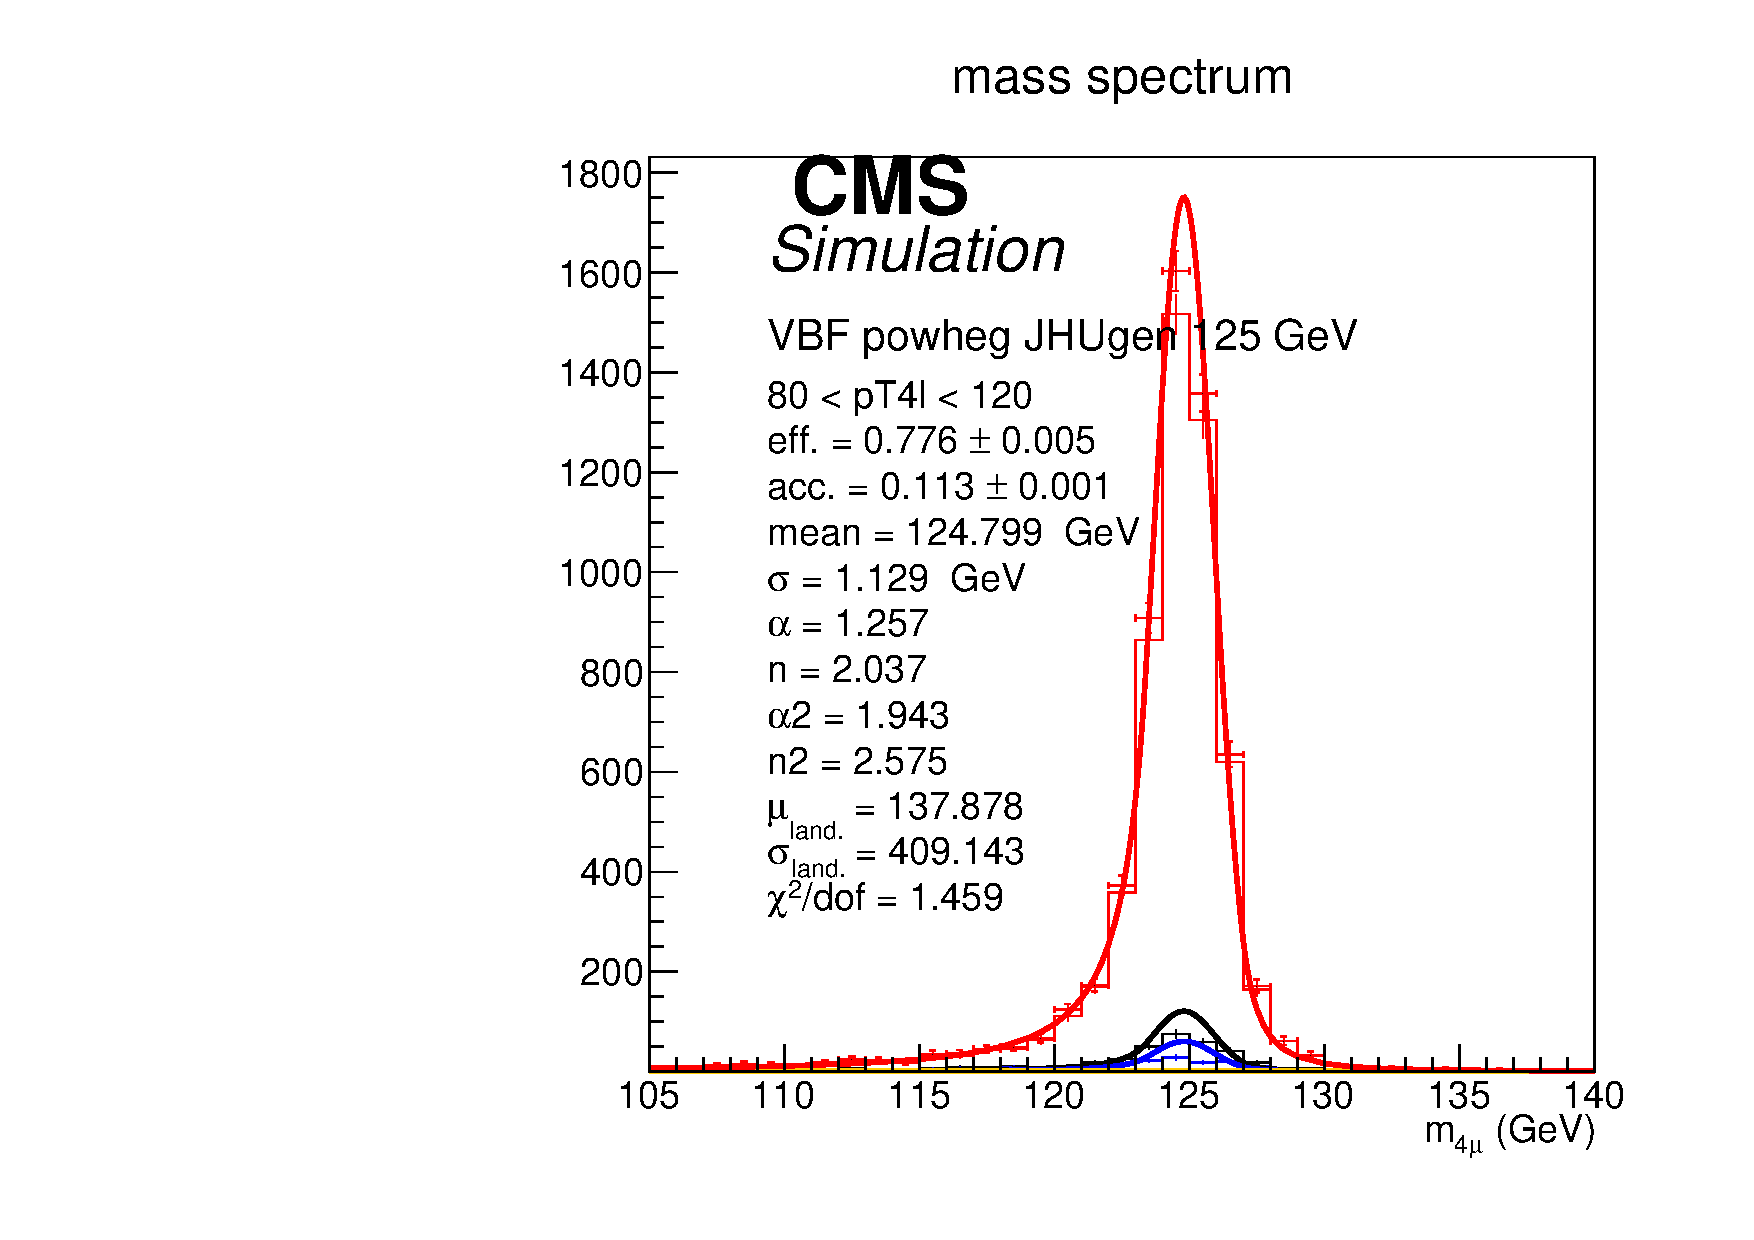
\includegraphics[width=0.3\textwidth,angle=0]{Figures/Appendix//VBF_powheg_JHUgen_125_4mu_pT4l_genbin4_recobin4_effs_genWeight*pileupWeight*dataMCWeight.pdf}
      \label{fig:sigfits-pT4l-VBF-powheg15-JHUgen-125-maintext:e}
    }
    \subfigure[$120.0 < \pt(\mathrm{H}) < 200.0$]{
      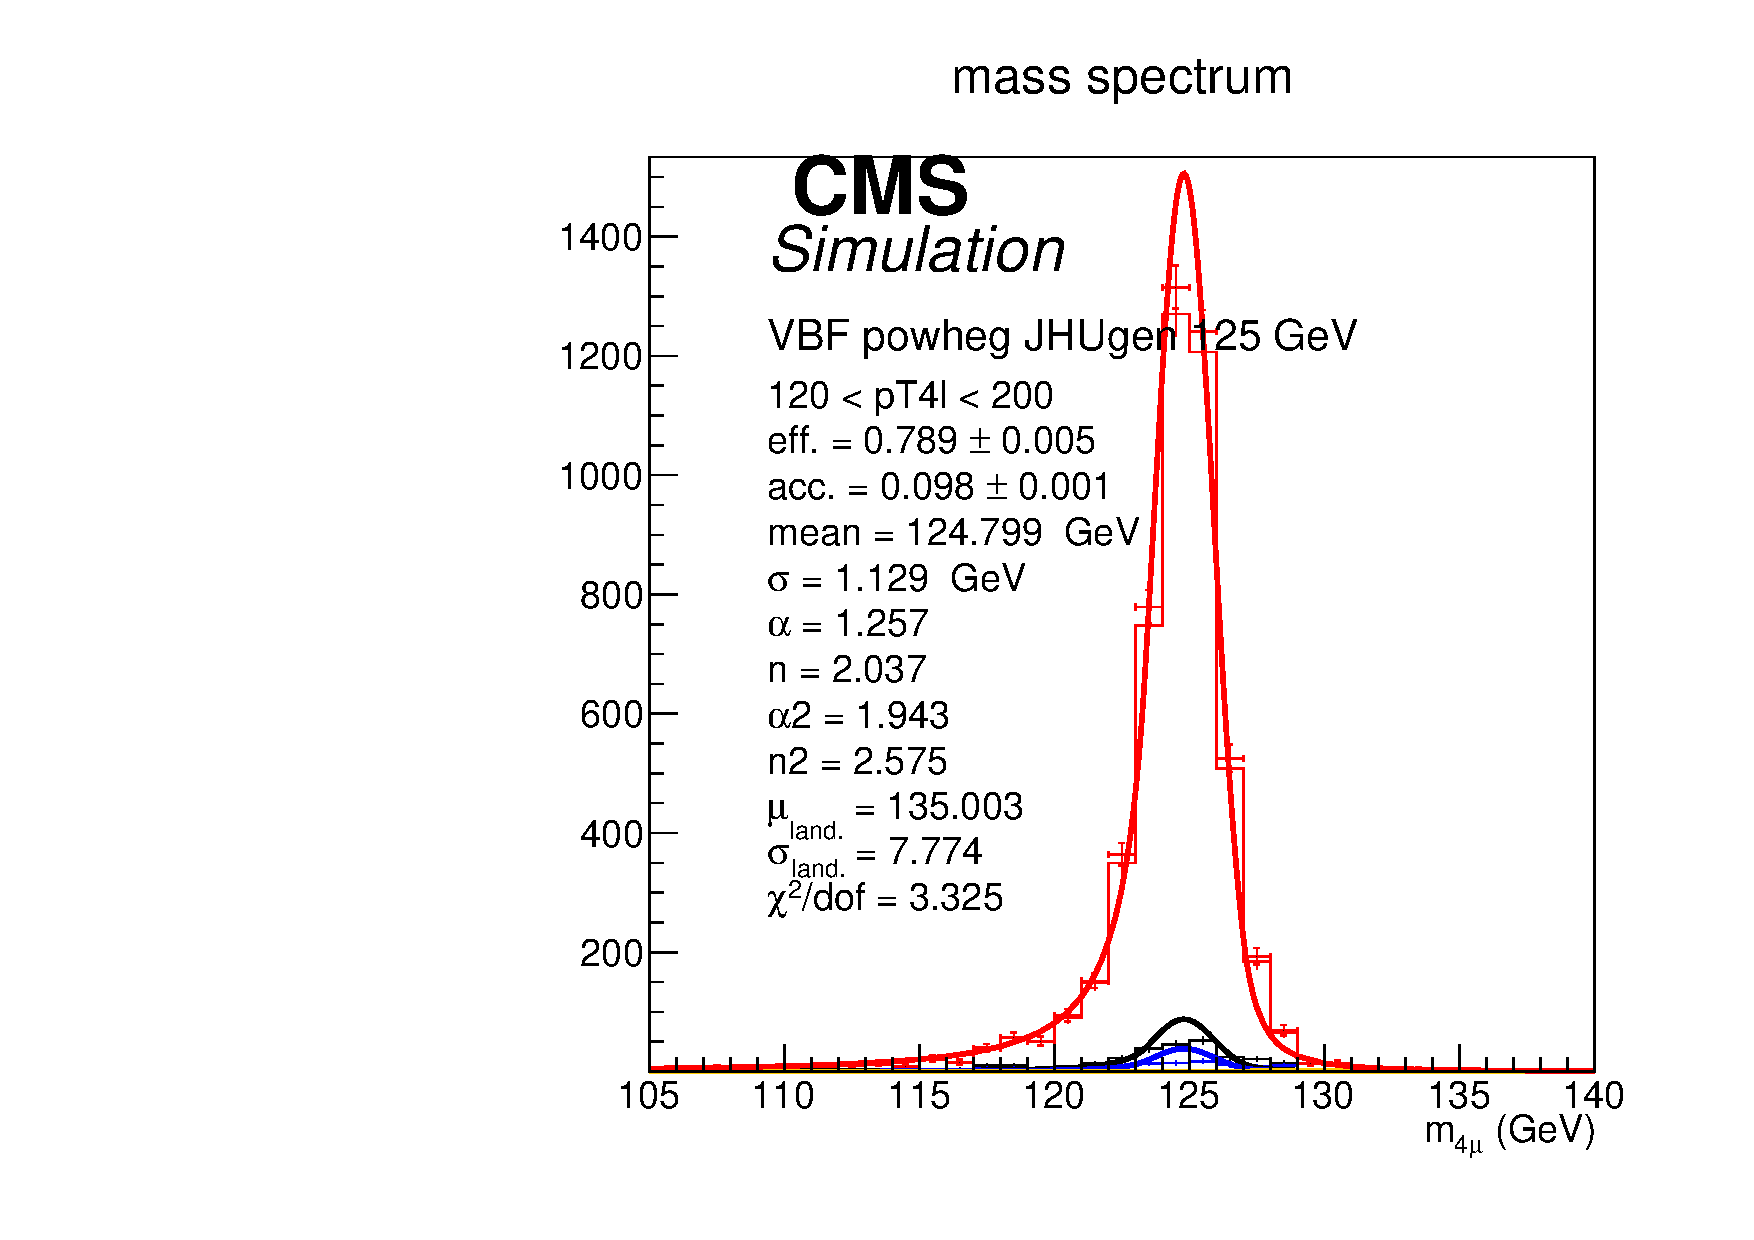
\includegraphics[width=0.3\textwidth,angle=0]{Figures/Appendix//VBF_powheg_JHUgen_125_4mu_pT4l_genbin5_recobin5_effs_genWeight*pileupWeight*dataMCWeight.pdf}
      \label{fig:sigfits-pT4l-VBF-powheg15-JHUgen-125-maintext:f}
    } \\
    \subfigure[$200.0 < \pt(\mathrm{H}) < 13000.0$]{
      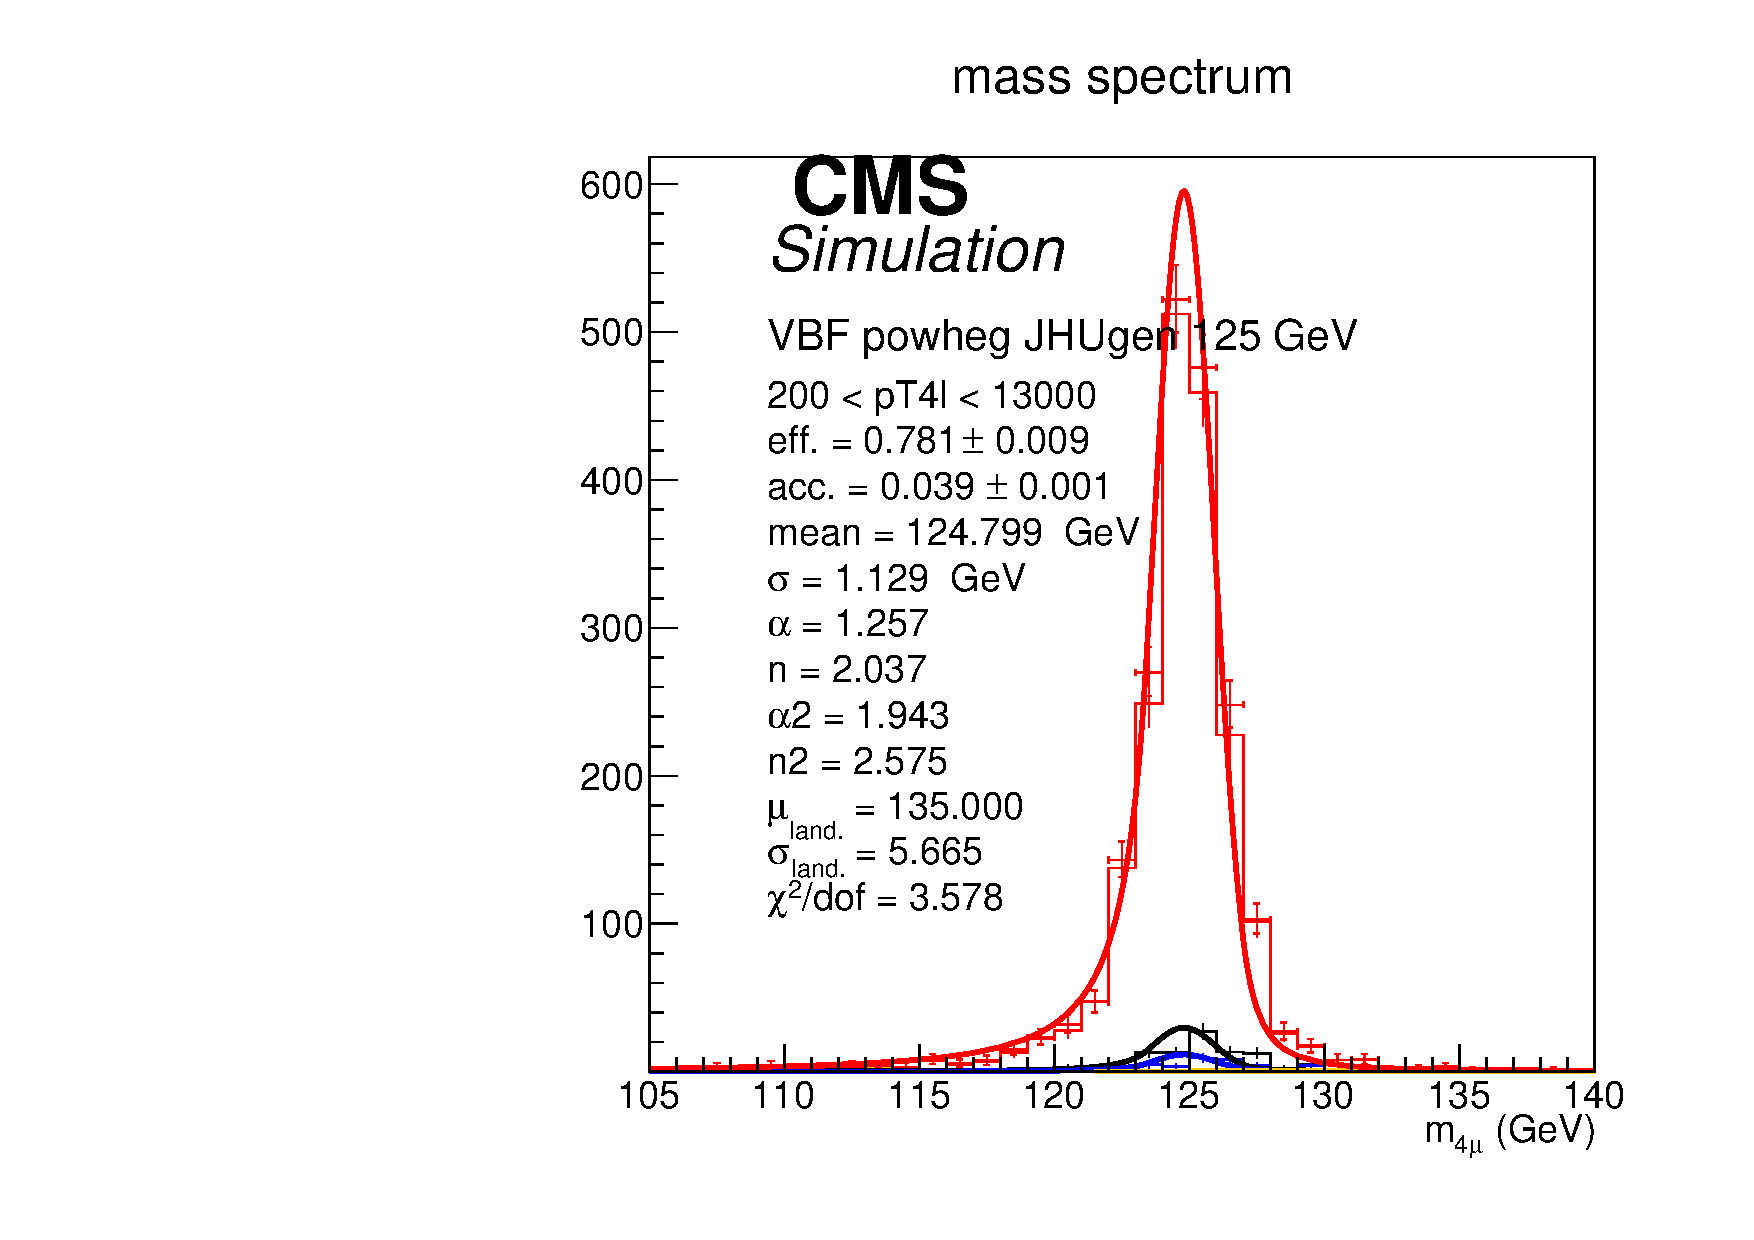
\includegraphics[width=0.3\textwidth,angle=0]{Figures/Appendix//VBF_powheg_JHUgen_125_4mu_pT4l_genbin6_recobin6_effs_genWeight*pileupWeight*dataMCWeight.pdf}
      \label{fig:sigfits-pT4l-VBF-powheg15-JHUgen-125-maintext:g}
    }
    \\
    \caption{ Example signal shapes at reconstruction level for a resonance of m(4$\ell$) in $4\mu$ final state for the $VBF$ production mode from {\sc powheg+JHUGen} in different bins of $\pt(\mathrm{H})$. The black curve represents events which do not pass the fiducial volume selection. The curve has no effect on the result.
    }
  \label{fig:sigfits-pT4l-VBF-powheg15-JHUgen-125-maintext}
 \end{center}
\end{figure} \clearpage


\begin{figure}[htb]
  \begin{center}
    \subfigure[$0.0 < \pt(\mathrm{H}) < 15.0 $]{
      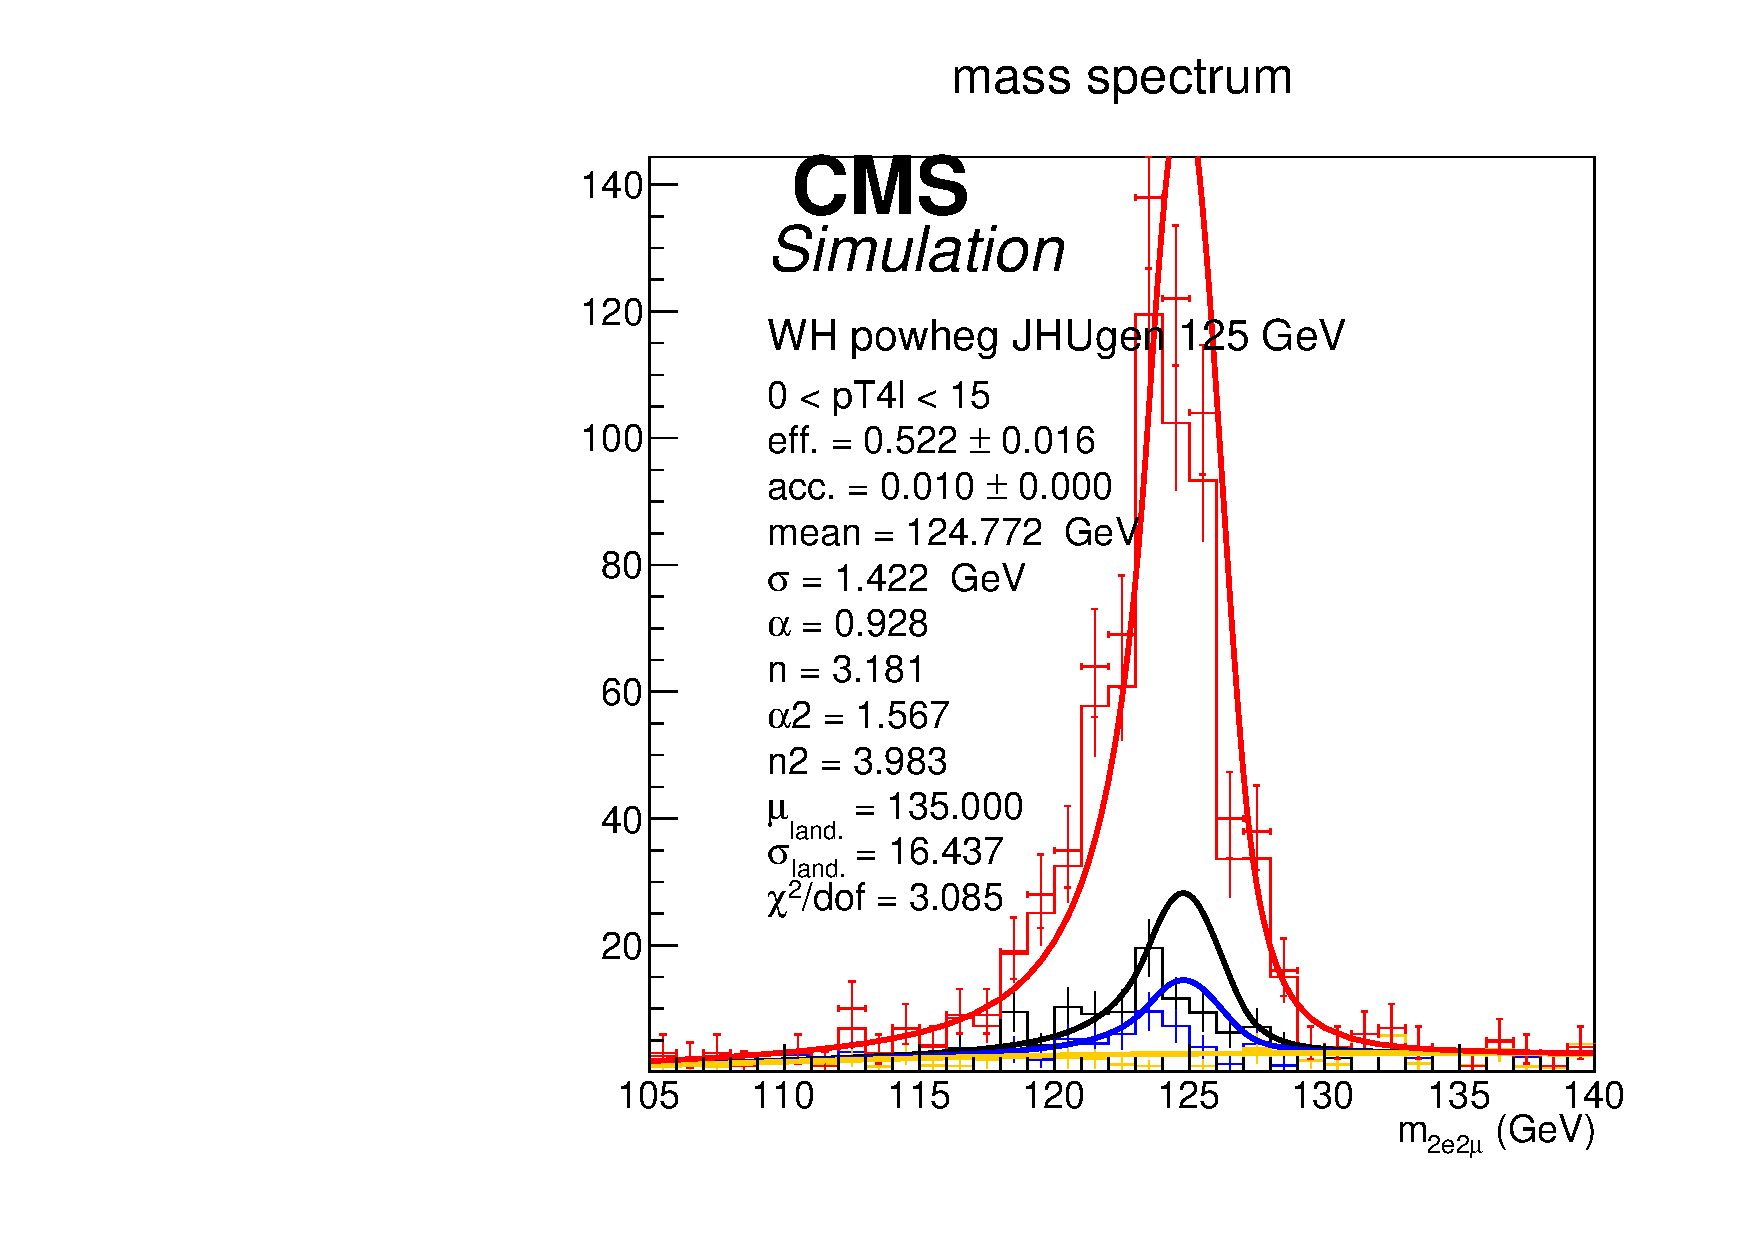
\includegraphics[width=0.3\textwidth,angle=0]{Figures/Appendix//WH_powheg_JHUgen_125_2e2mu_pT4l_genbin0_recobin0_effs_genWeight*pileupWeight*dataMCWeight.pdf}
      \label{fig:sigfits-pT4l-WH-powheg15-JHUgen-125-maintext:a}
    }
    \subfigure[$15.0 < \pt(\mathrm{H}) < 30.0$]{
      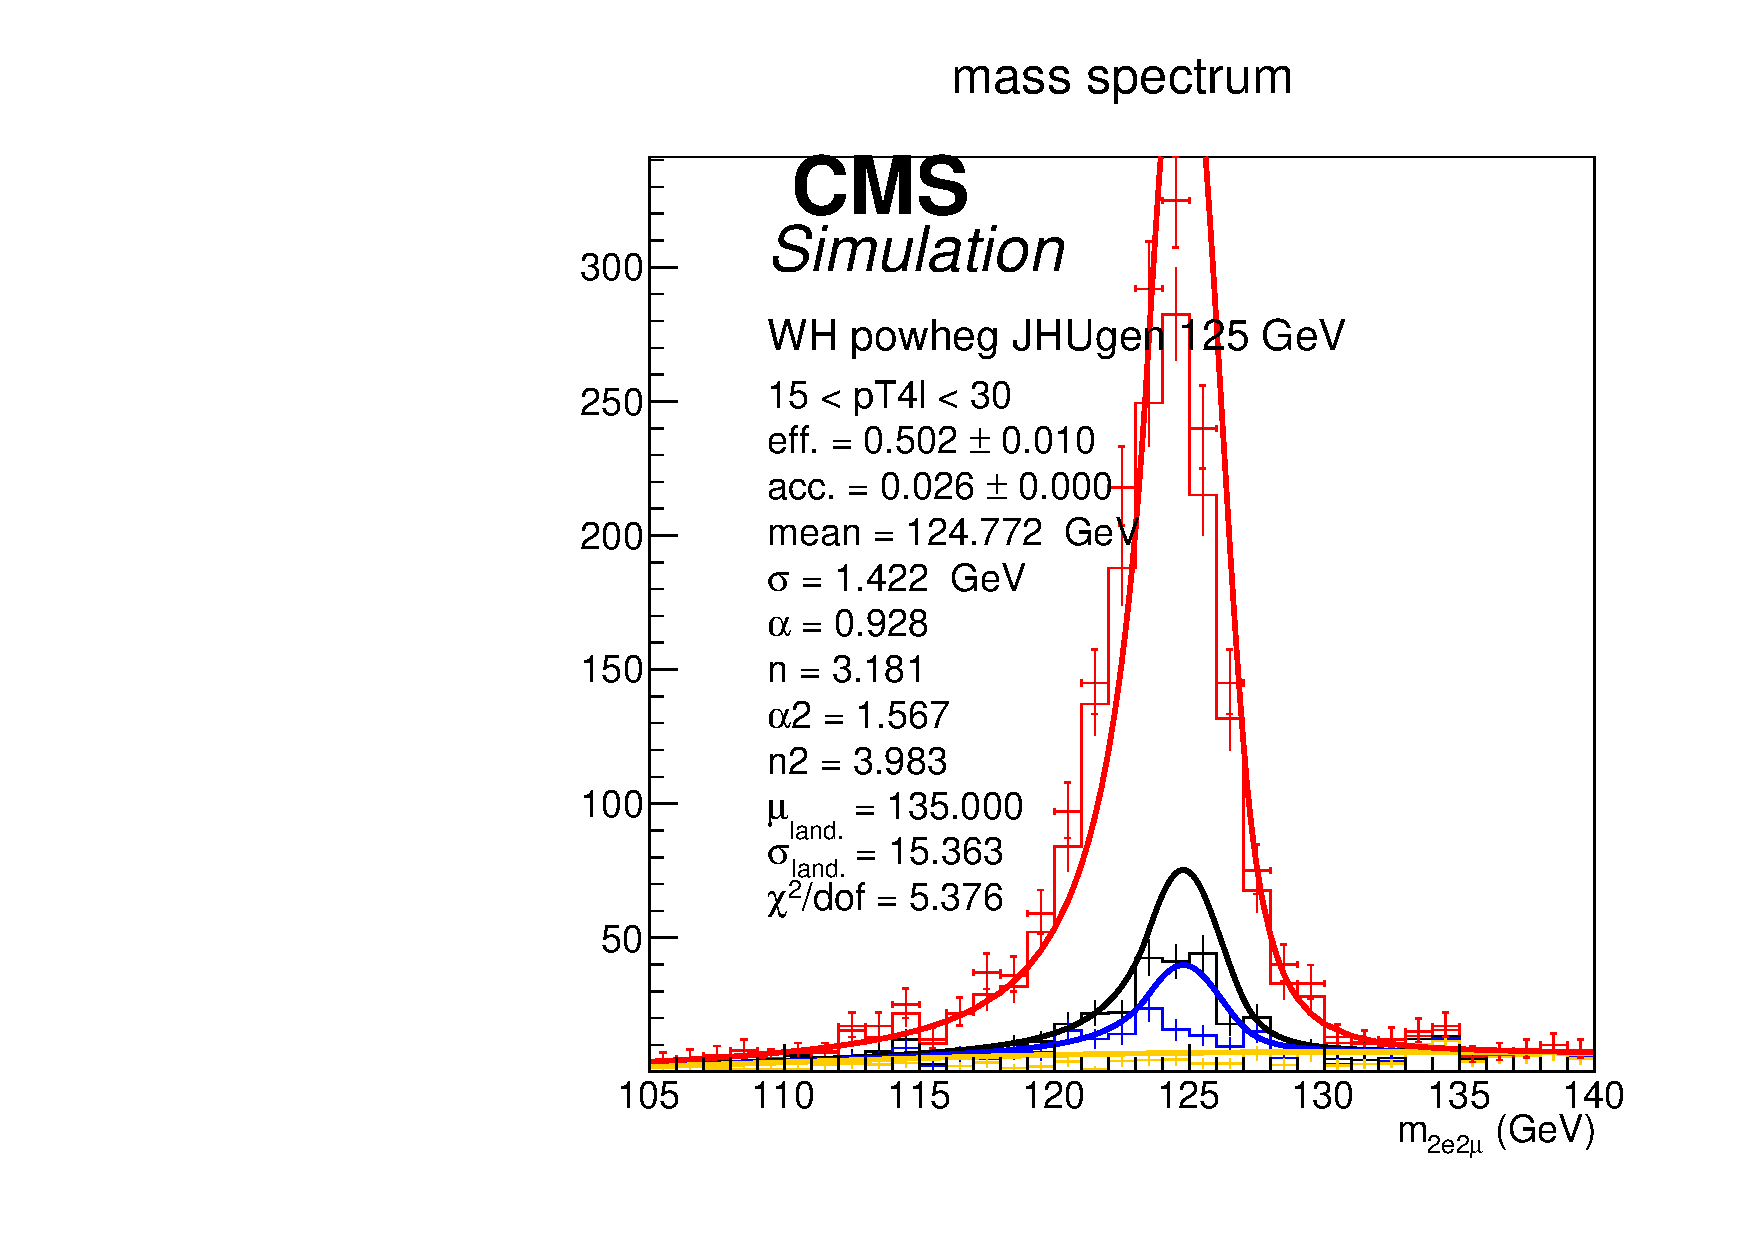
\includegraphics[width=0.3\textwidth,angle=0]{Figures/Appendix//WH_powheg_JHUgen_125_2e2mu_pT4l_genbin1_recobin1_effs_genWeight*pileupWeight*dataMCWeight.pdf}
      \label{fig:sigfits-pT4l-WH-powheg15-JHUgen-125-maintext:b}
    }
   \subfigure[$30.0 < \pt(\mathrm{H}) < 45.0$]{
      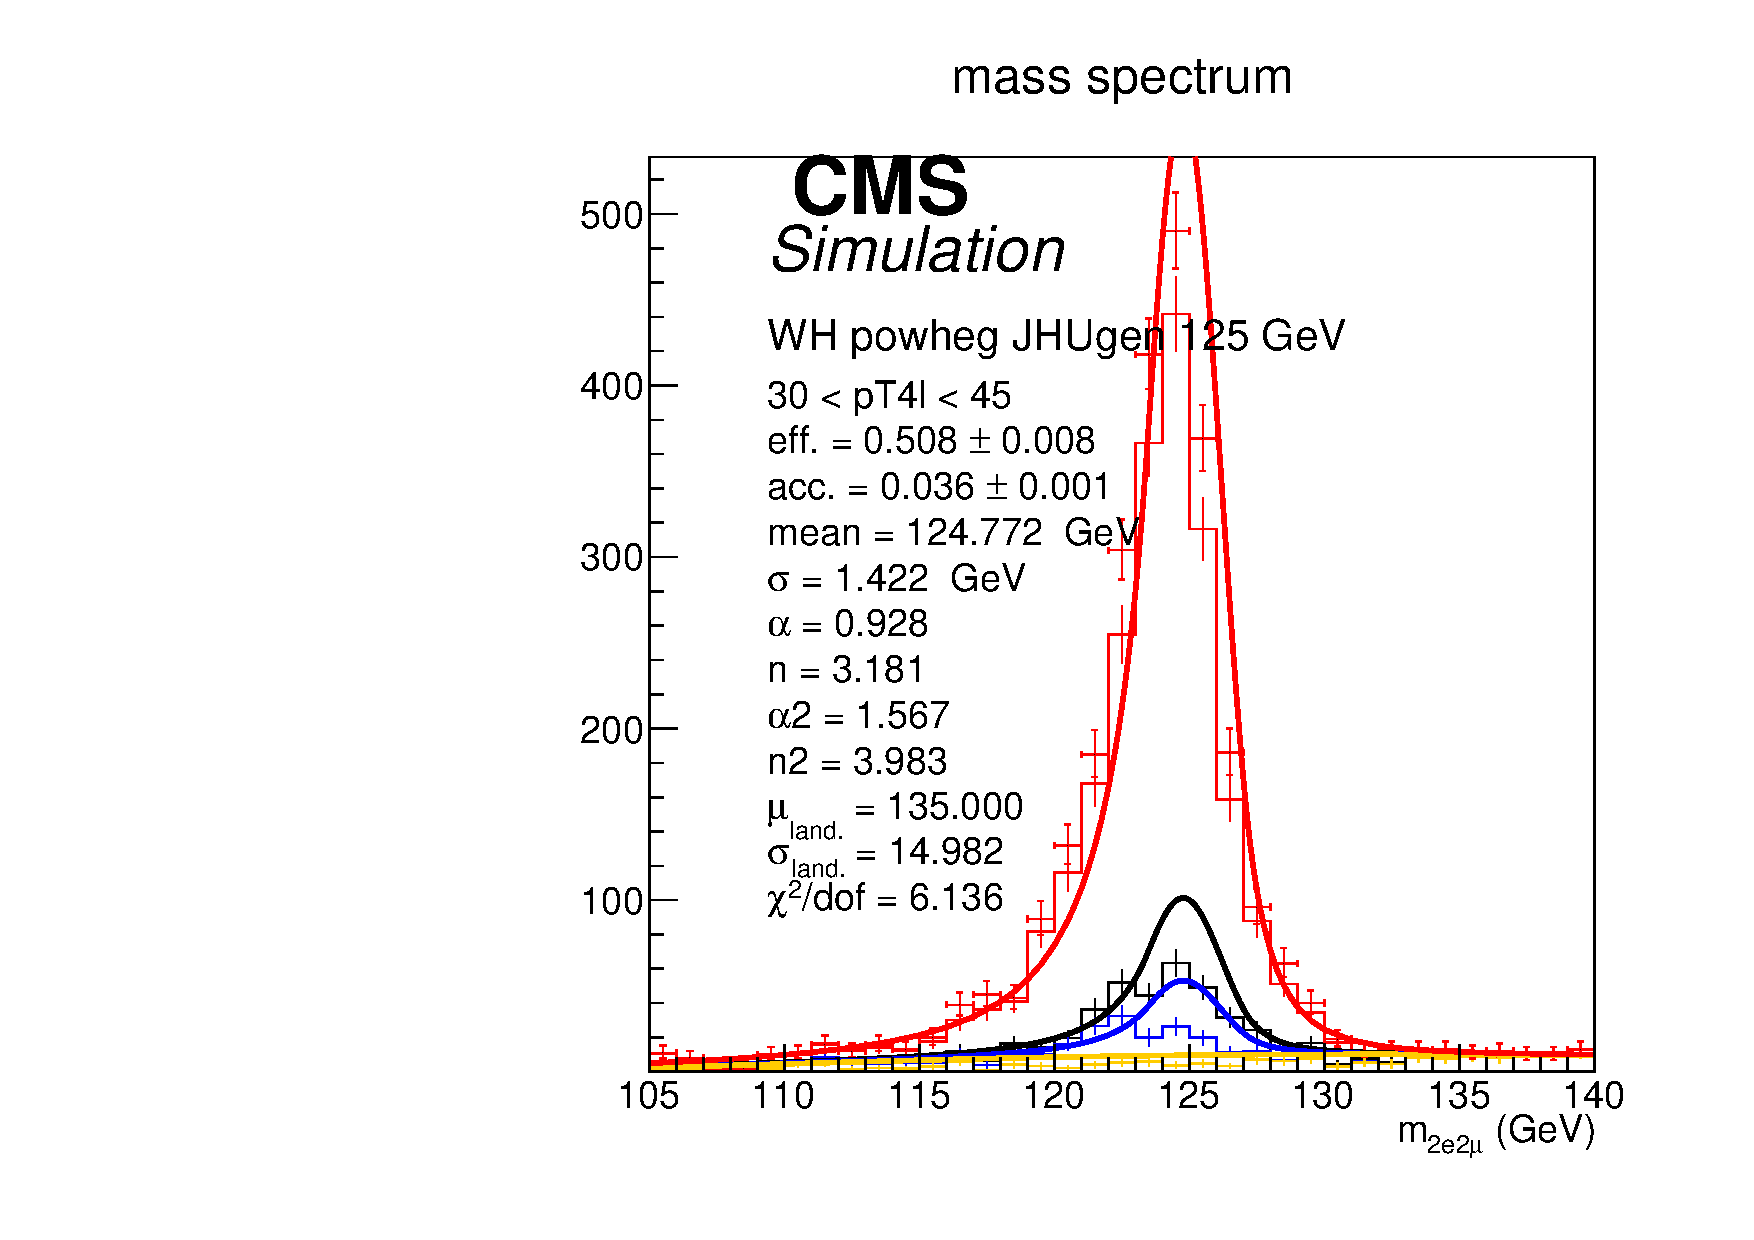
\includegraphics[width=0.3\textwidth,angle=0]{Figures/Appendix//WH_powheg_JHUgen_125_2e2mu_pT4l_genbin2_recobin2_effs_genWeight*pileupWeight*dataMCWeight.pdf}
      \label{fig:sigfits-pT4l-WH-powheg15-JHUgen-125-maintext:c}
    }  \\
    \subfigure[$45.0 < \pt(\mathrm{H}) < 80.0$]{
      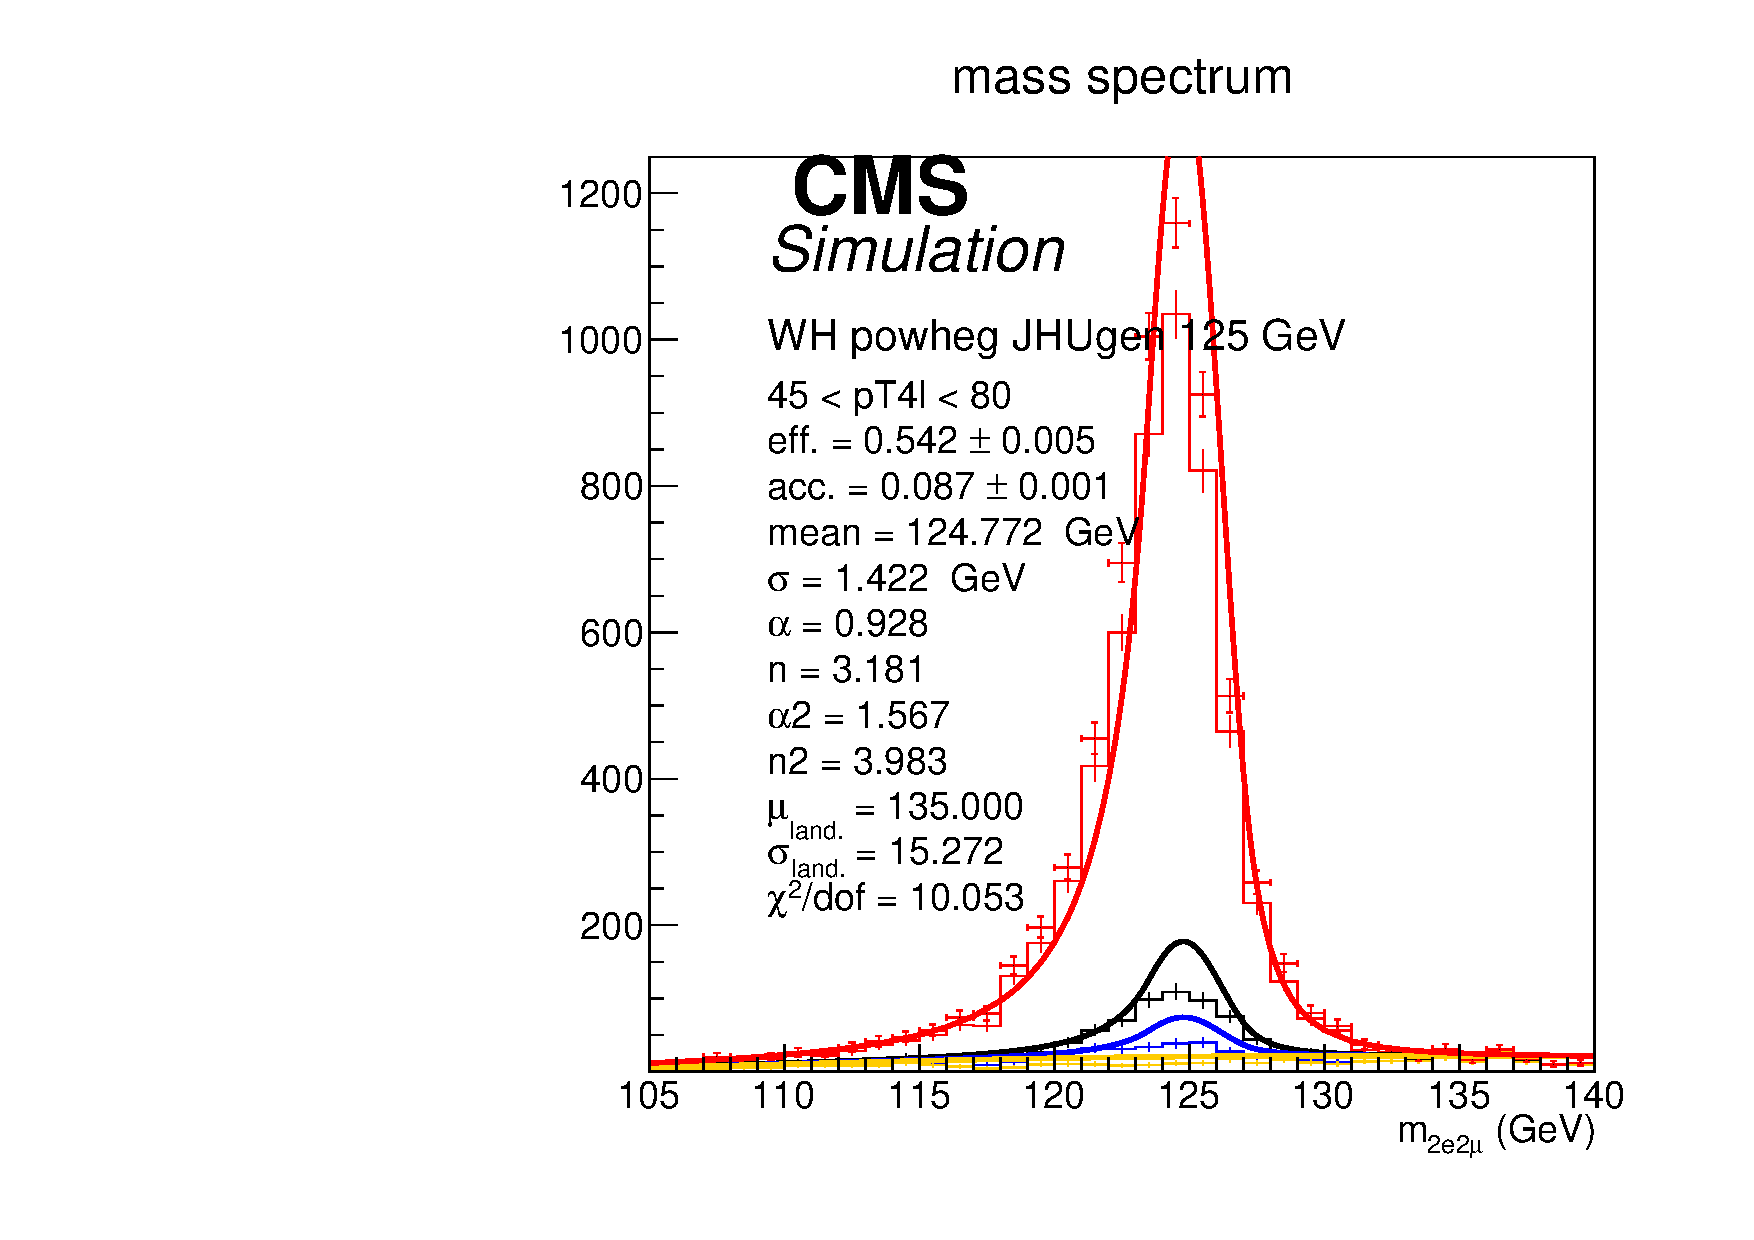
\includegraphics[width=0.3\textwidth,angle=0]{Figures/Appendix//WH_powheg_JHUgen_125_2e2mu_pT4l_genbin3_recobin3_effs_genWeight*pileupWeight*dataMCWeight.pdf}
      \label{fig:sigfits-pT4l-WH-powheg15-JHUgen-125-maintext:d}
    }
    \subfigure[$80.0 < \pt(\mathrm{H}) < 120.0$]{
      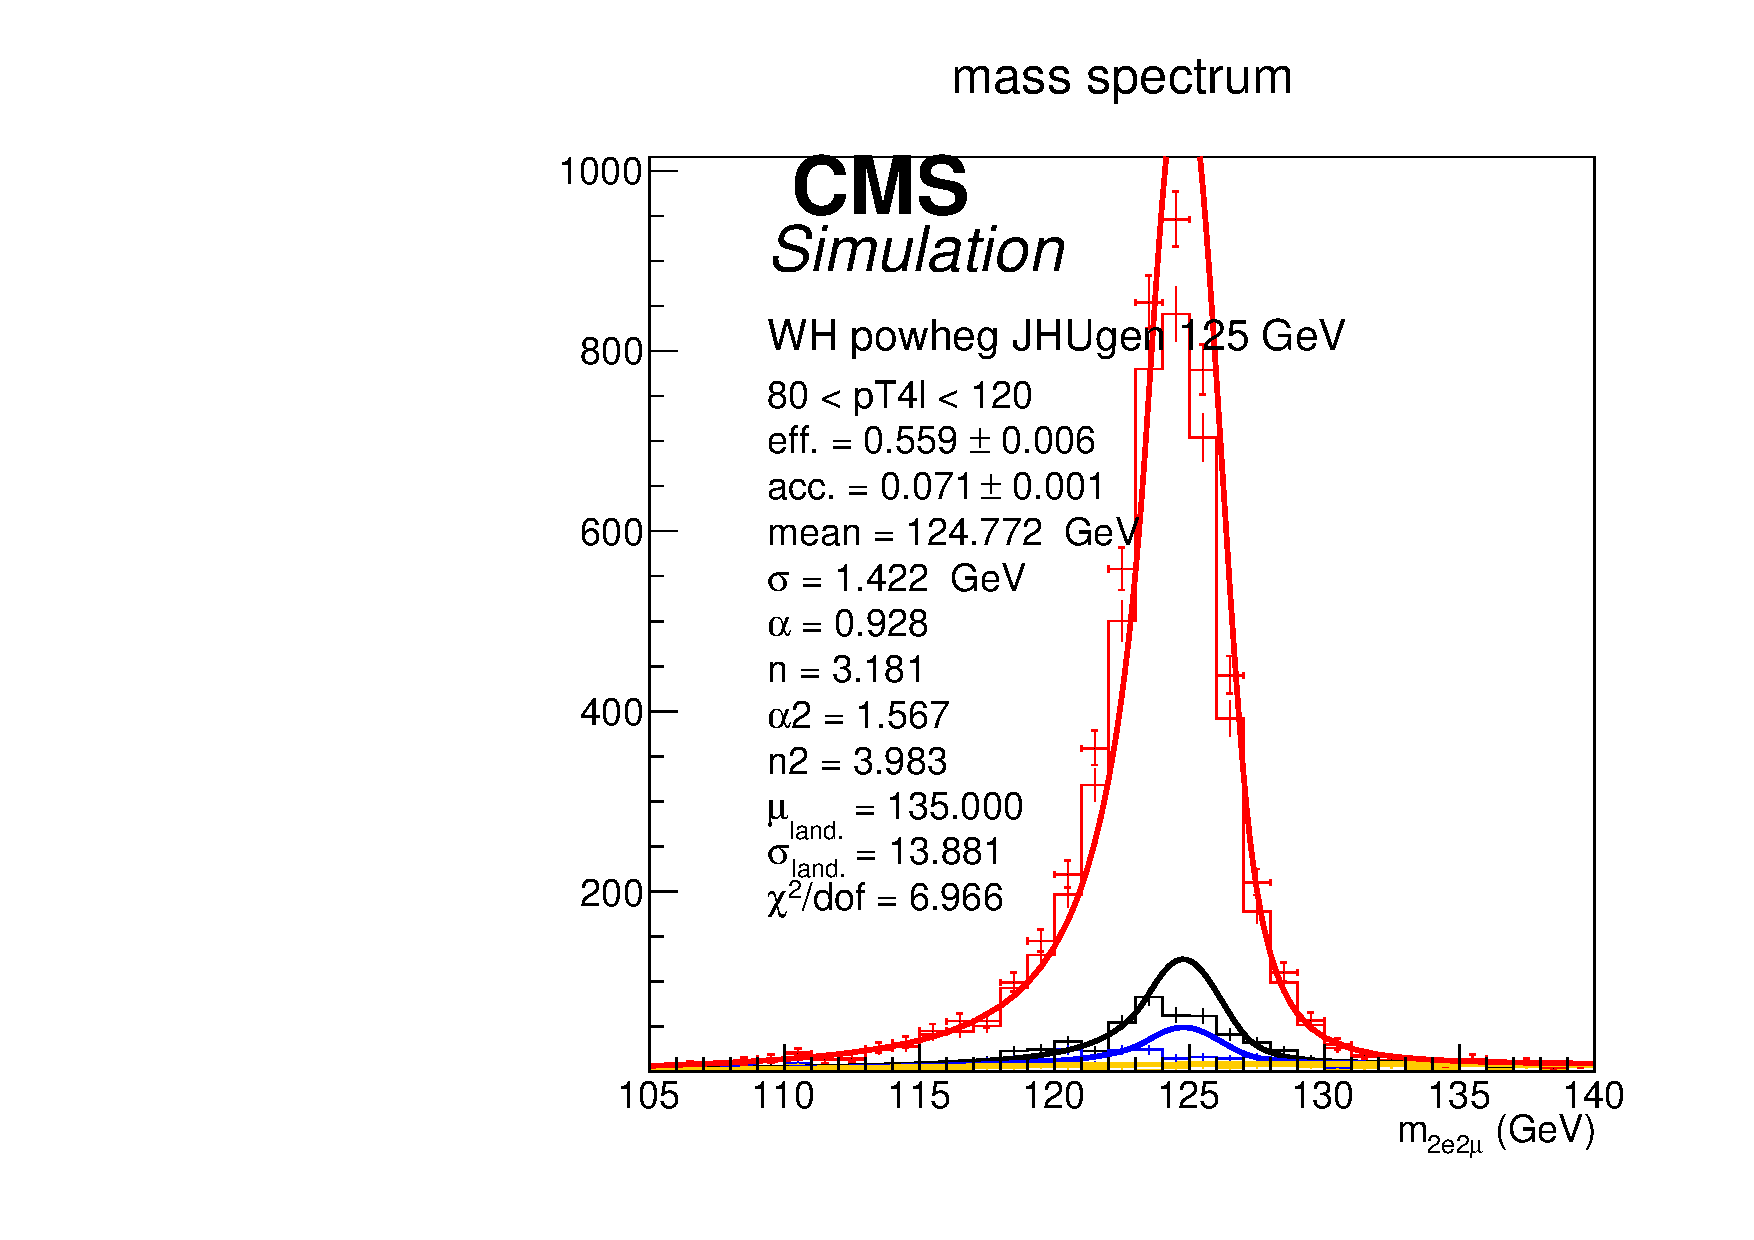
\includegraphics[width=0.3\textwidth,angle=0]{Figures/Appendix//WH_powheg_JHUgen_125_2e2mu_pT4l_genbin4_recobin4_effs_genWeight*pileupWeight*dataMCWeight.pdf}
      \label{fig:sigfits-pT4l-WH-powheg15-JHUgen-125-maintext:e}
    }
    \subfigure[$120.0 < \pt(\mathrm{H}) < 200.0$]{
      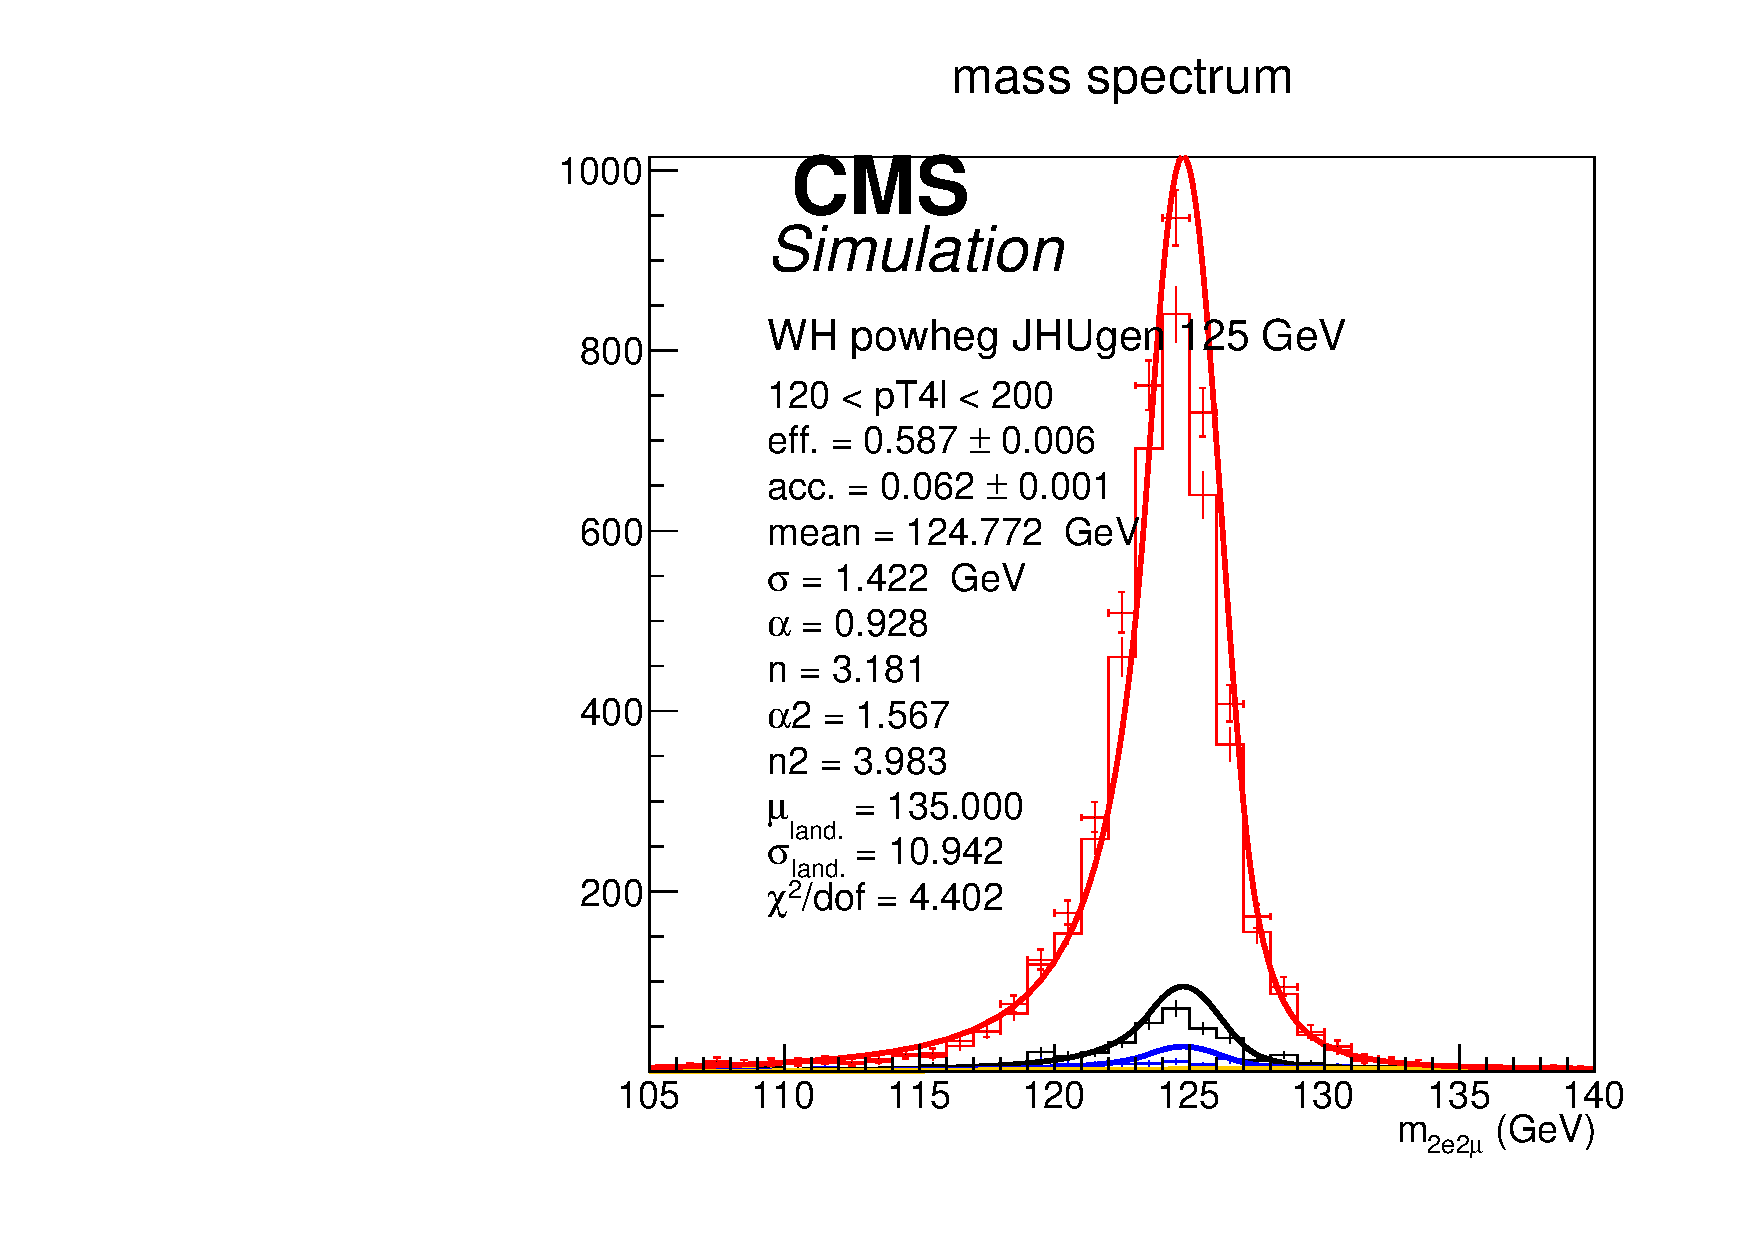
\includegraphics[width=0.3\textwidth,angle=0]{Figures/Appendix//WH_powheg_JHUgen_125_2e2mu_pT4l_genbin5_recobin5_effs_genWeight*pileupWeight*dataMCWeight.pdf}
      \label{fig:sigfits-pT4l-WH-powheg15-JHUgen-125-maintext:f}
    } \\
    \subfigure[$200.0 < \pt(\mathrm{H}) < 13000.0$]{
      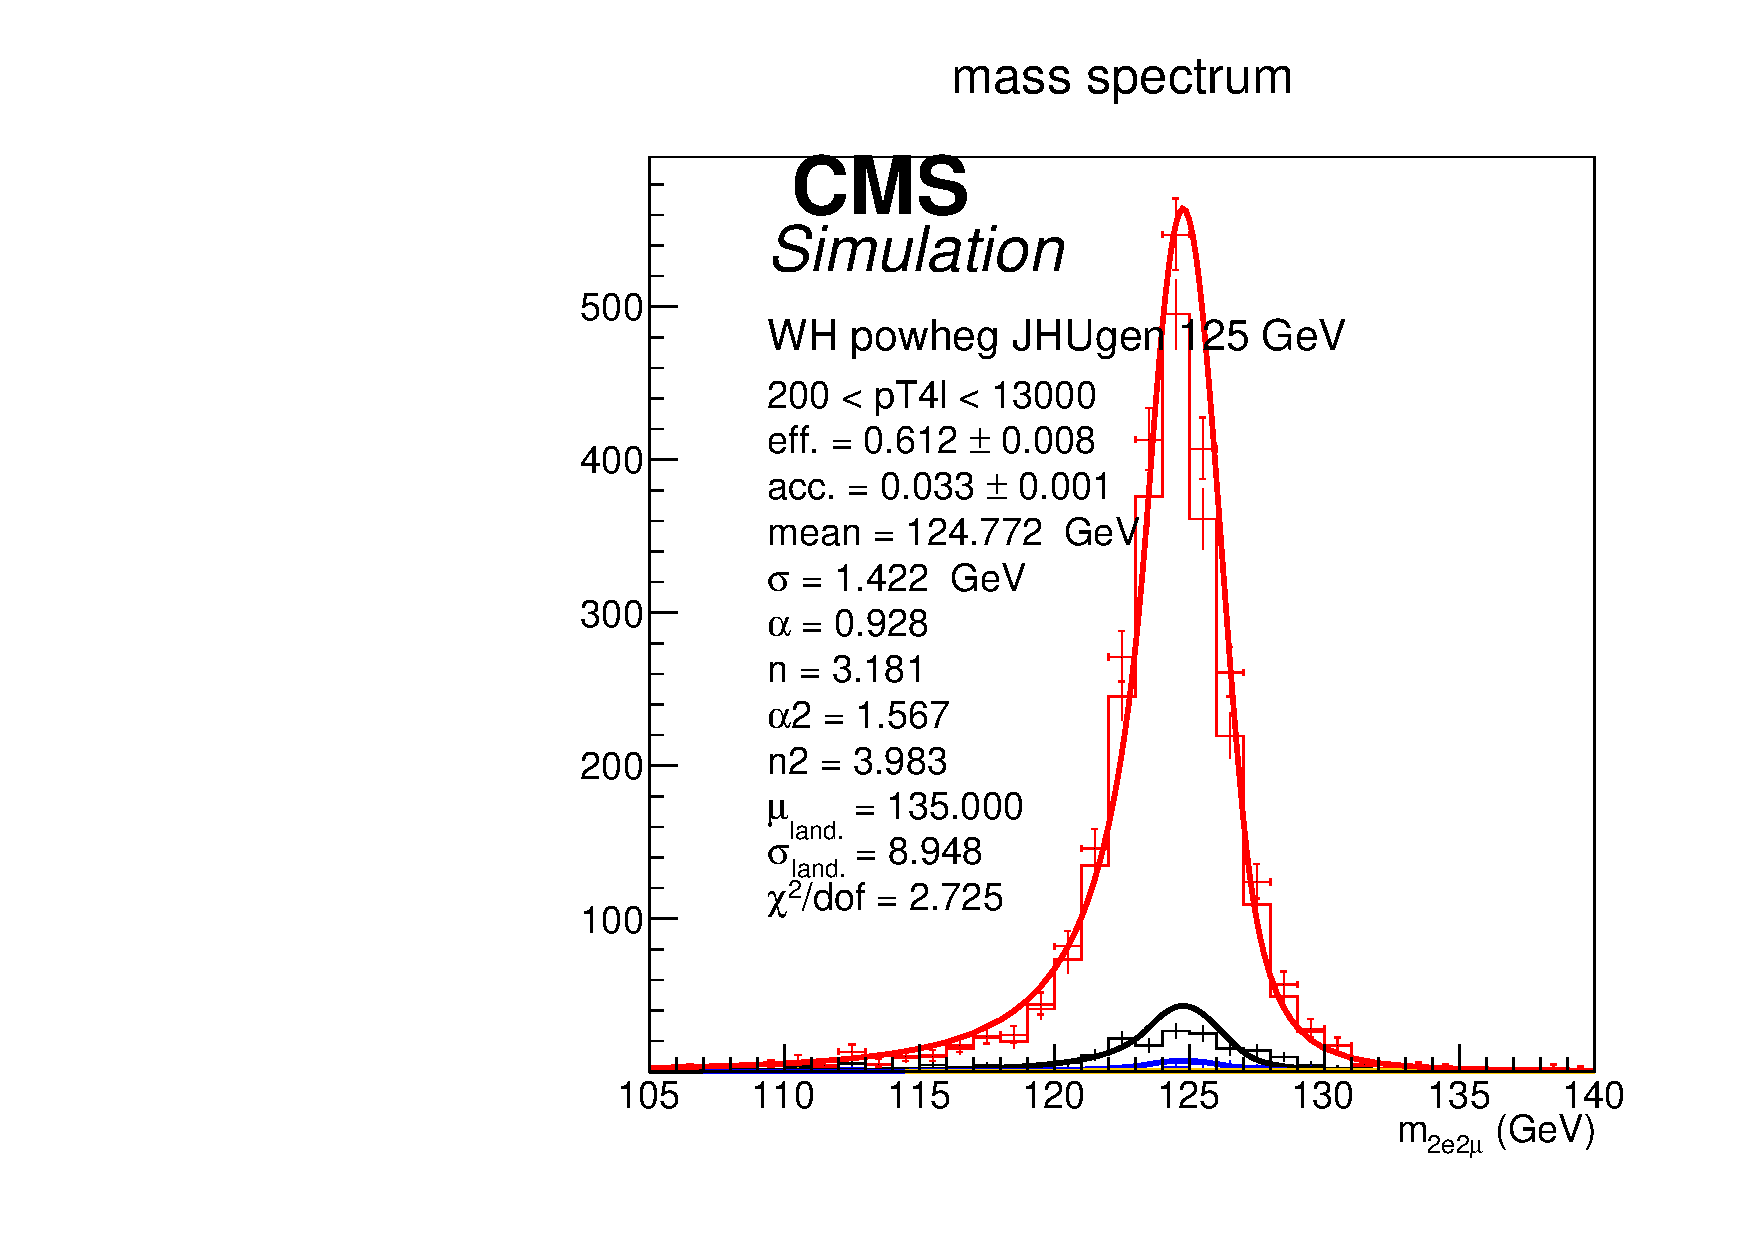
\includegraphics[width=0.3\textwidth,angle=0]{Figures/Appendix//WH_powheg_JHUgen_125_2e2mu_pT4l_genbin6_recobin6_effs_genWeight*pileupWeight*dataMCWeight.pdf}
      \label{fig:sigfits-pT4l-WH-powheg15-JHUgen-125-maintext:g}
    }
    \\
    \caption{ Example signal shapes at reconstruction level for a resonance of m(4$\ell$) in $2e2\mu$ final state for the $WH$ production mode from {\sc powheg+JHUGen} in different bins of $\pt(\mathrm{H})$. The black curve represents events which do not pass the fiducial volume selection. The curve has no effect on the result.
    }
  \label{fig:sigfits-pT4l-WH-powheg15-JHUgen-125-maintext}
 \end{center}
\end{figure} \clearpage

\begin{figure}[htb]
  \begin{center}
    \subfigure[$0.0 < \pt(\mathrm{H}) < 15.0 $]{
      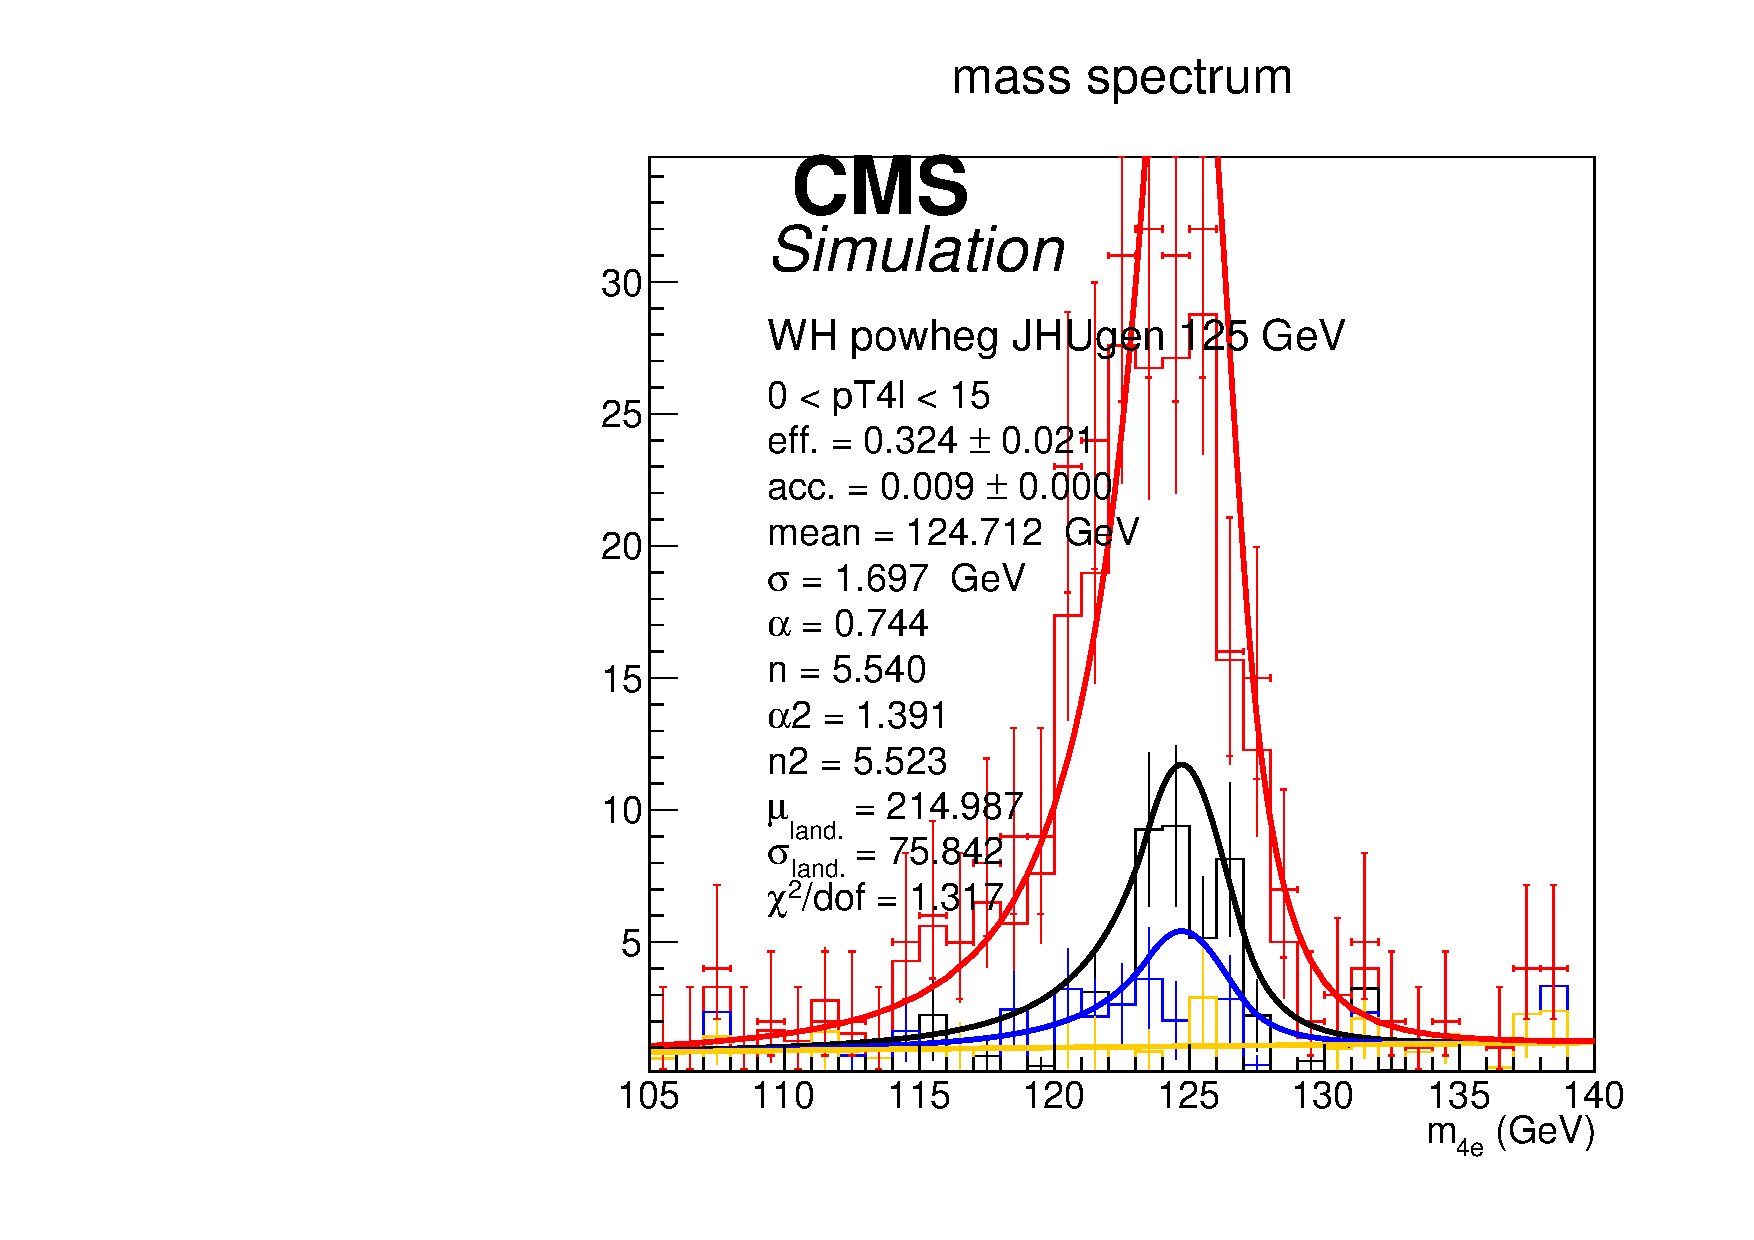
\includegraphics[width=0.3\textwidth,angle=0]{Figures/Appendix//WH_powheg_JHUgen_125_4e_pT4l_genbin0_recobin0_effs_genWeight*pileupWeight*dataMCWeight.pdf}
      \label{fig:sigfits-pT4l-WH-powheg15-JHUgen-125-maintext:a}
    }
    \subfigure[$15.0 < \pt(\mathrm{H}) < 30.0$]{
      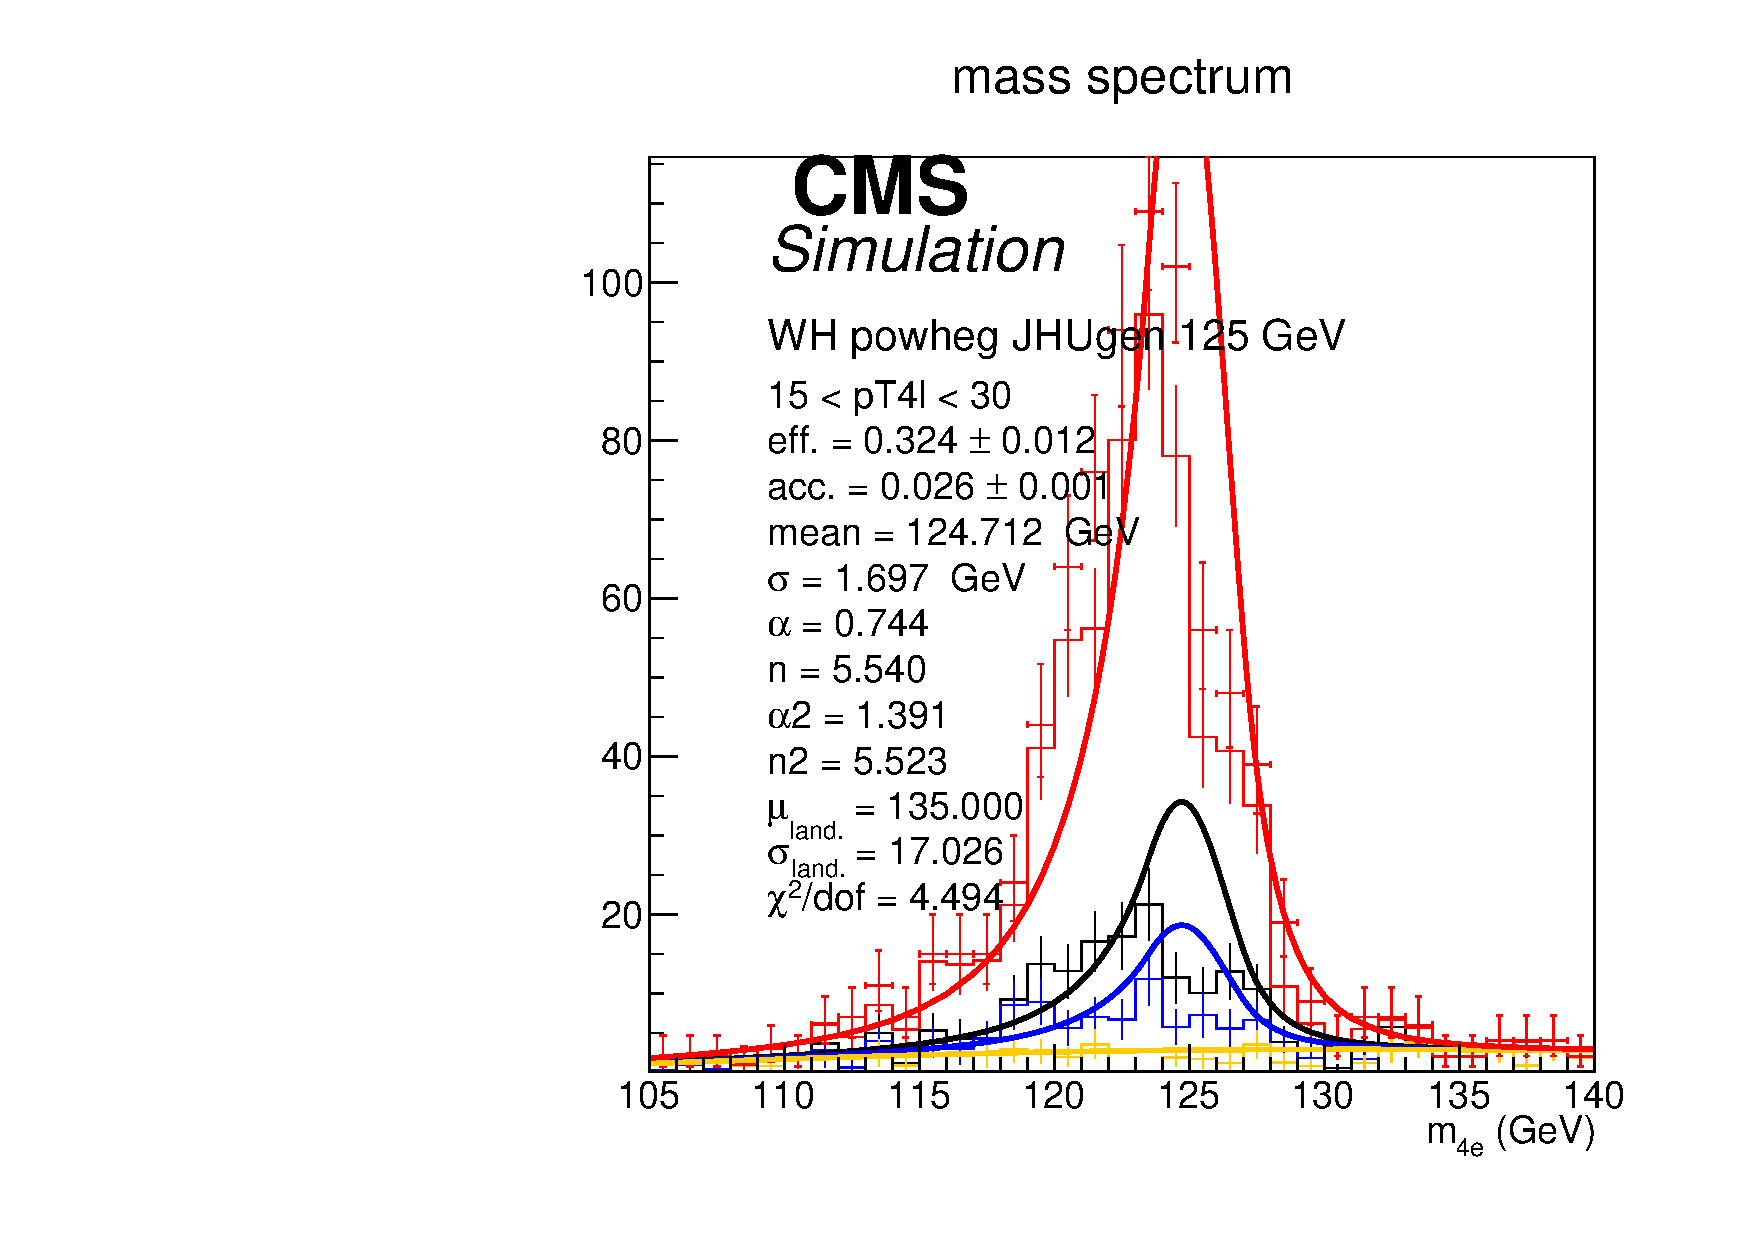
\includegraphics[width=0.3\textwidth,angle=0]{Figures/Appendix//WH_powheg_JHUgen_125_4e_pT4l_genbin1_recobin1_effs_genWeight*pileupWeight*dataMCWeight.pdf}
      \label{fig:sigfits-pT4l-WH-powheg15-JHUgen-125-maintext:b}
    }
   \subfigure[$30.0 < \pt(\mathrm{H}) < 45.0$]{
      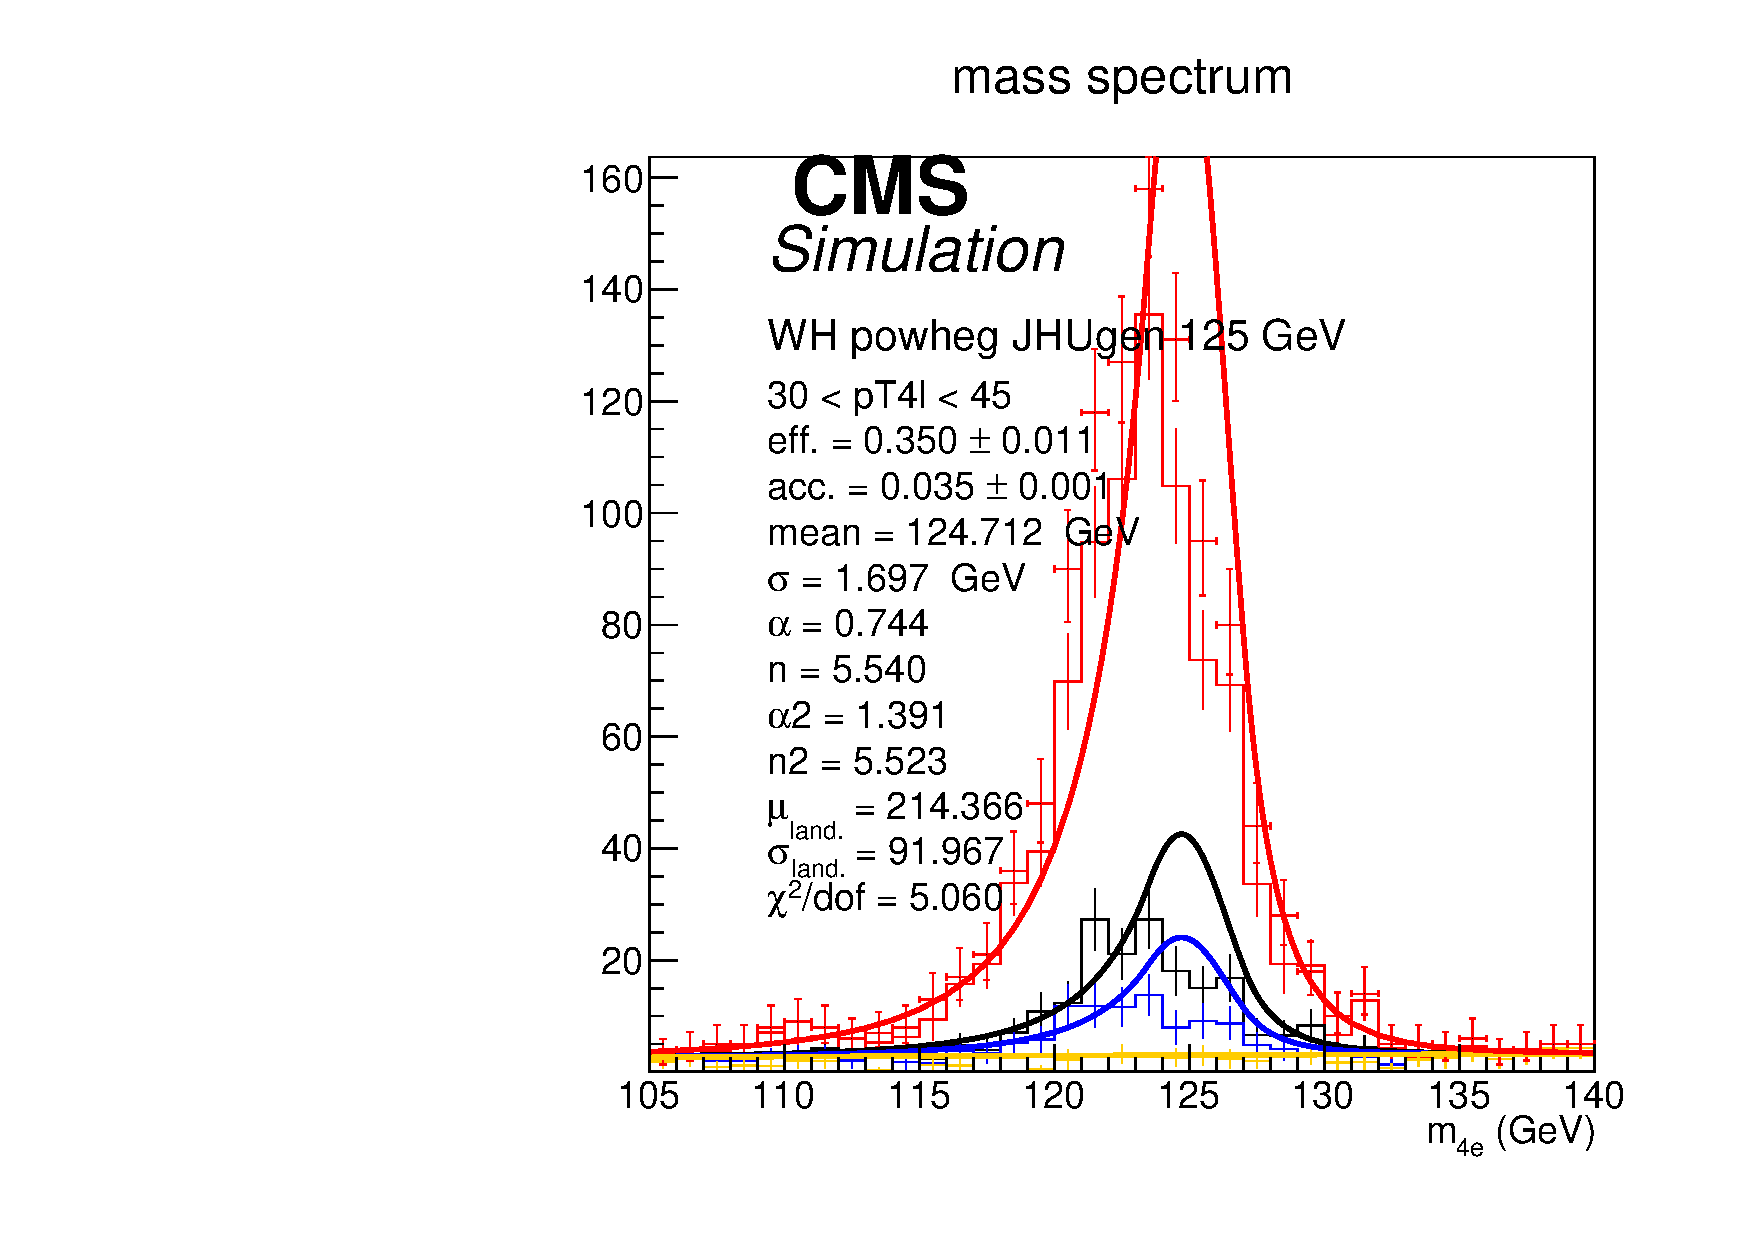
\includegraphics[width=0.3\textwidth,angle=0]{Figures/Appendix//WH_powheg_JHUgen_125_4e_pT4l_genbin2_recobin2_effs_genWeight*pileupWeight*dataMCWeight.pdf}
      \label{fig:sigfits-pT4l-WH-powheg15-JHUgen-125-maintext:c}
    }  \\
    \subfigure[$45.0 < \pt(\mathrm{H}) < 80.0$]{
      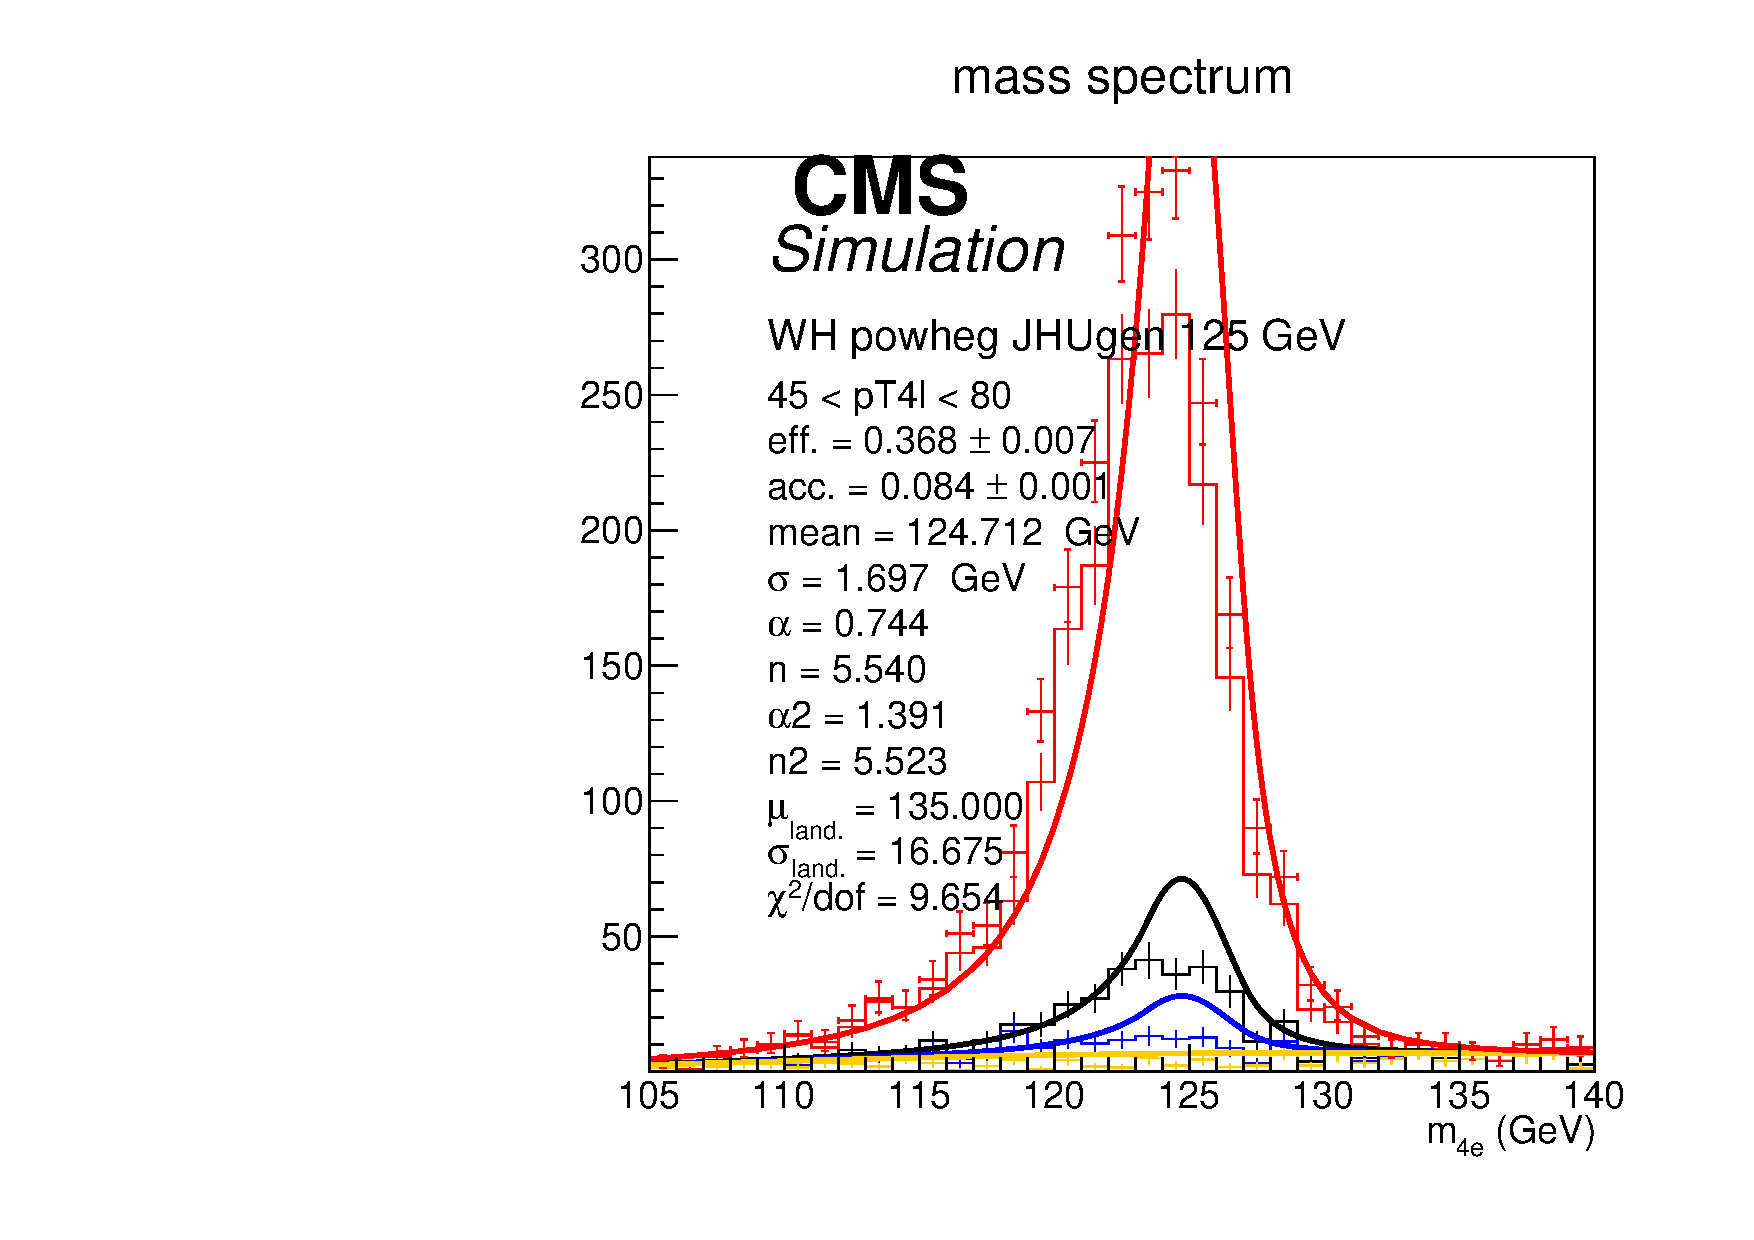
\includegraphics[width=0.3\textwidth,angle=0]{Figures/Appendix//WH_powheg_JHUgen_125_4e_pT4l_genbin3_recobin3_effs_genWeight*pileupWeight*dataMCWeight.pdf}
      \label{fig:sigfits-pT4l-WH-powheg15-JHUgen-125-maintext:d}
    }
    \subfigure[$80.0 < \pt(\mathrm{H}) < 120.0$]{
      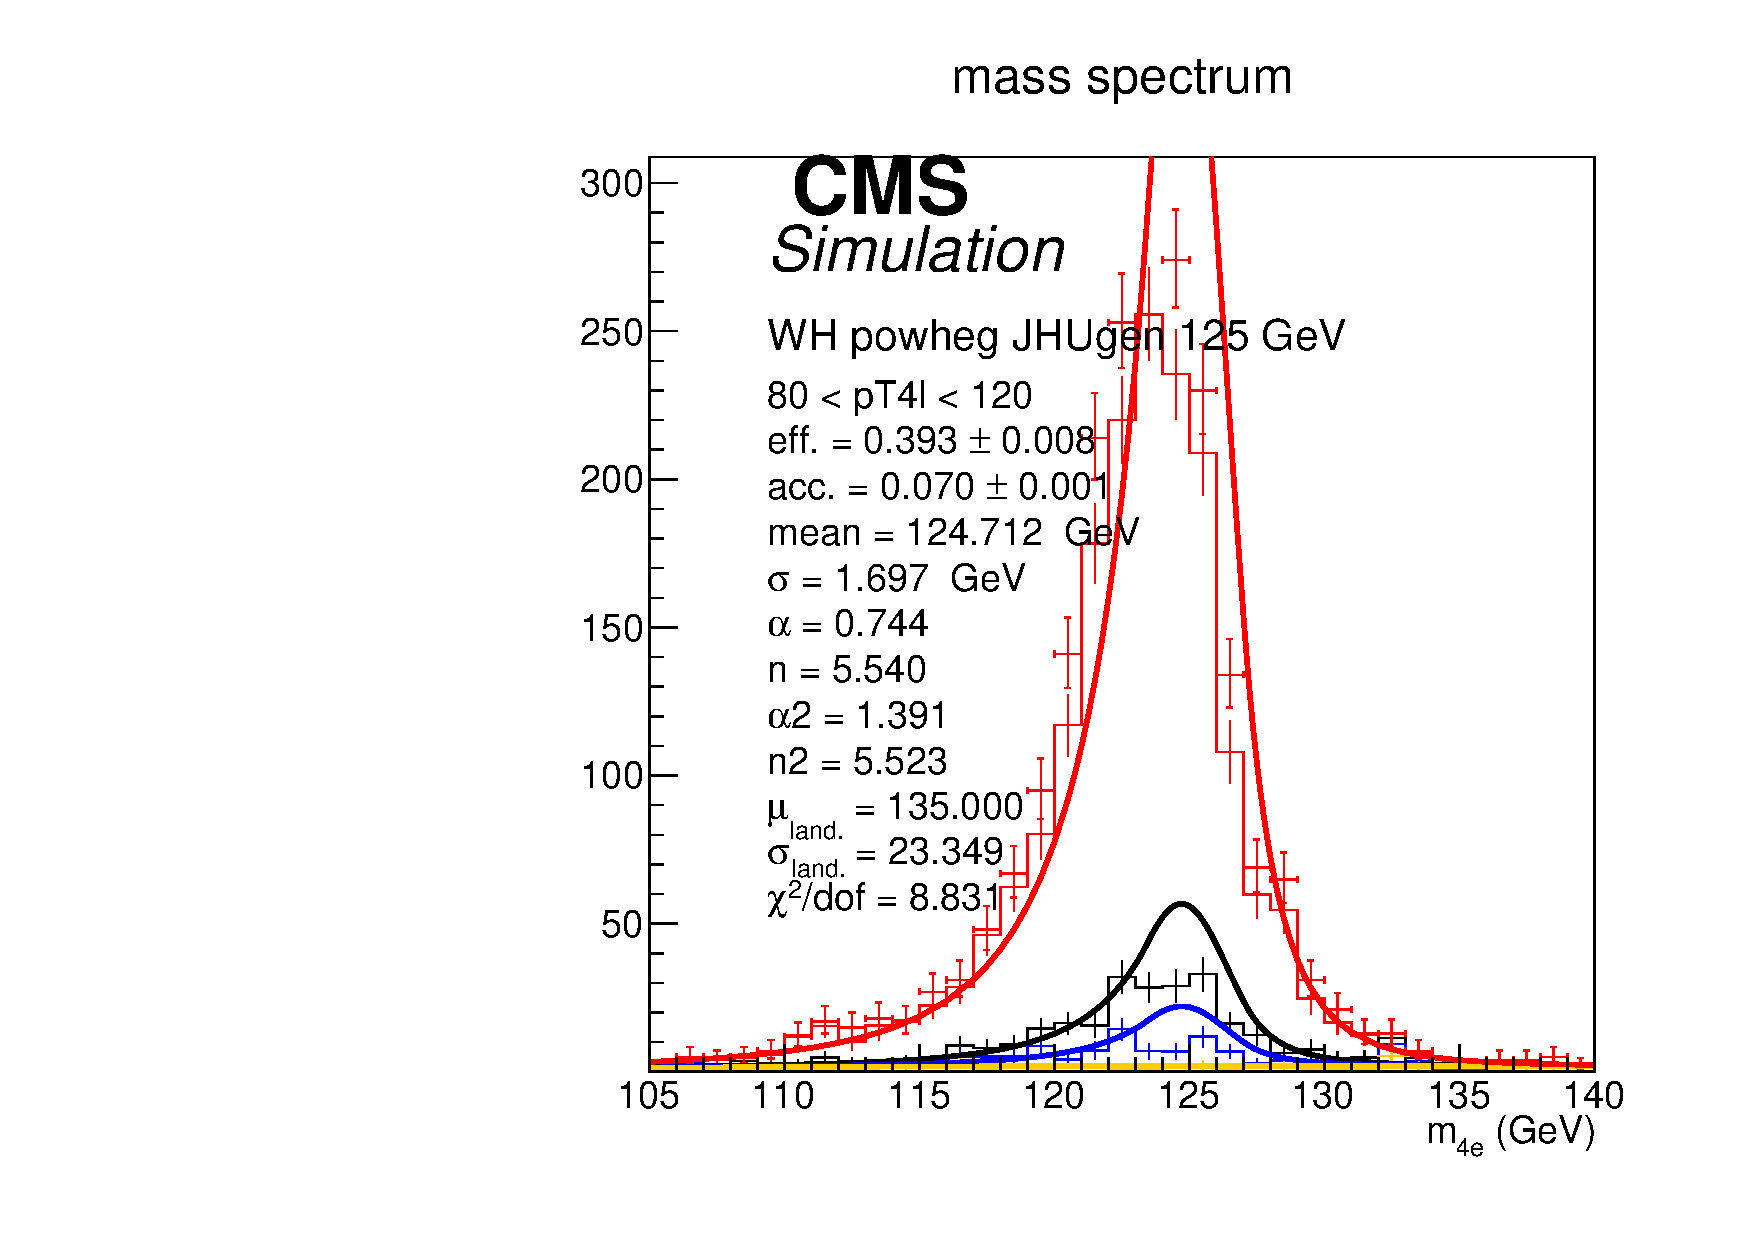
\includegraphics[width=0.3\textwidth,angle=0]{Figures/Appendix//WH_powheg_JHUgen_125_4e_pT4l_genbin4_recobin4_effs_genWeight*pileupWeight*dataMCWeight.pdf}
      \label{fig:sigfits-pT4l-WH-powheg15-JHUgen-125-maintext:e}
    }
    \subfigure[$120.0 < \pt(\mathrm{H}) < 200.0$]{
      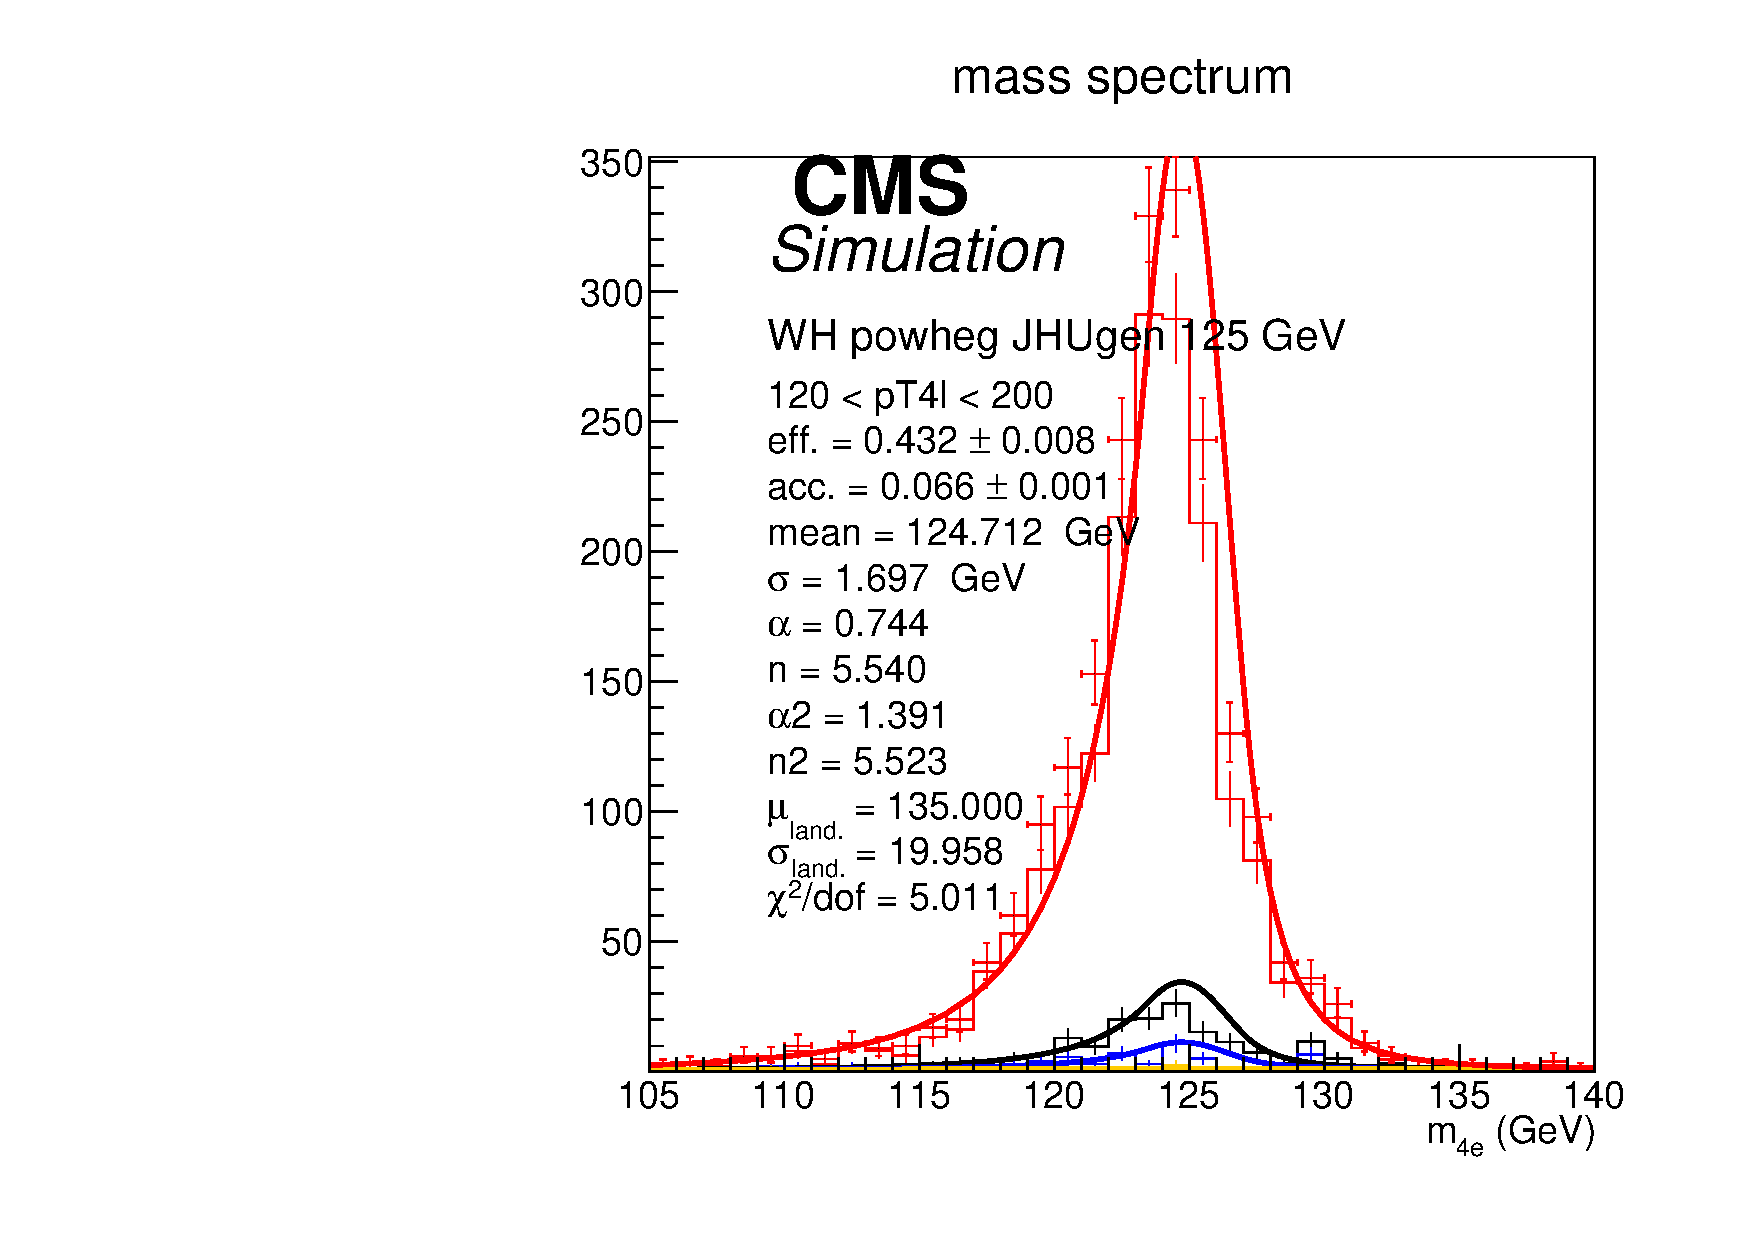
\includegraphics[width=0.3\textwidth,angle=0]{Figures/Appendix//WH_powheg_JHUgen_125_4e_pT4l_genbin5_recobin5_effs_genWeight*pileupWeight*dataMCWeight.pdf}
      \label{fig:sigfits-pT4l-WH-powheg15-JHUgen-125-maintext:f}
    } \\
    \subfigure[$200.0 < \pt(\mathrm{H}) < 13000.0$]{
      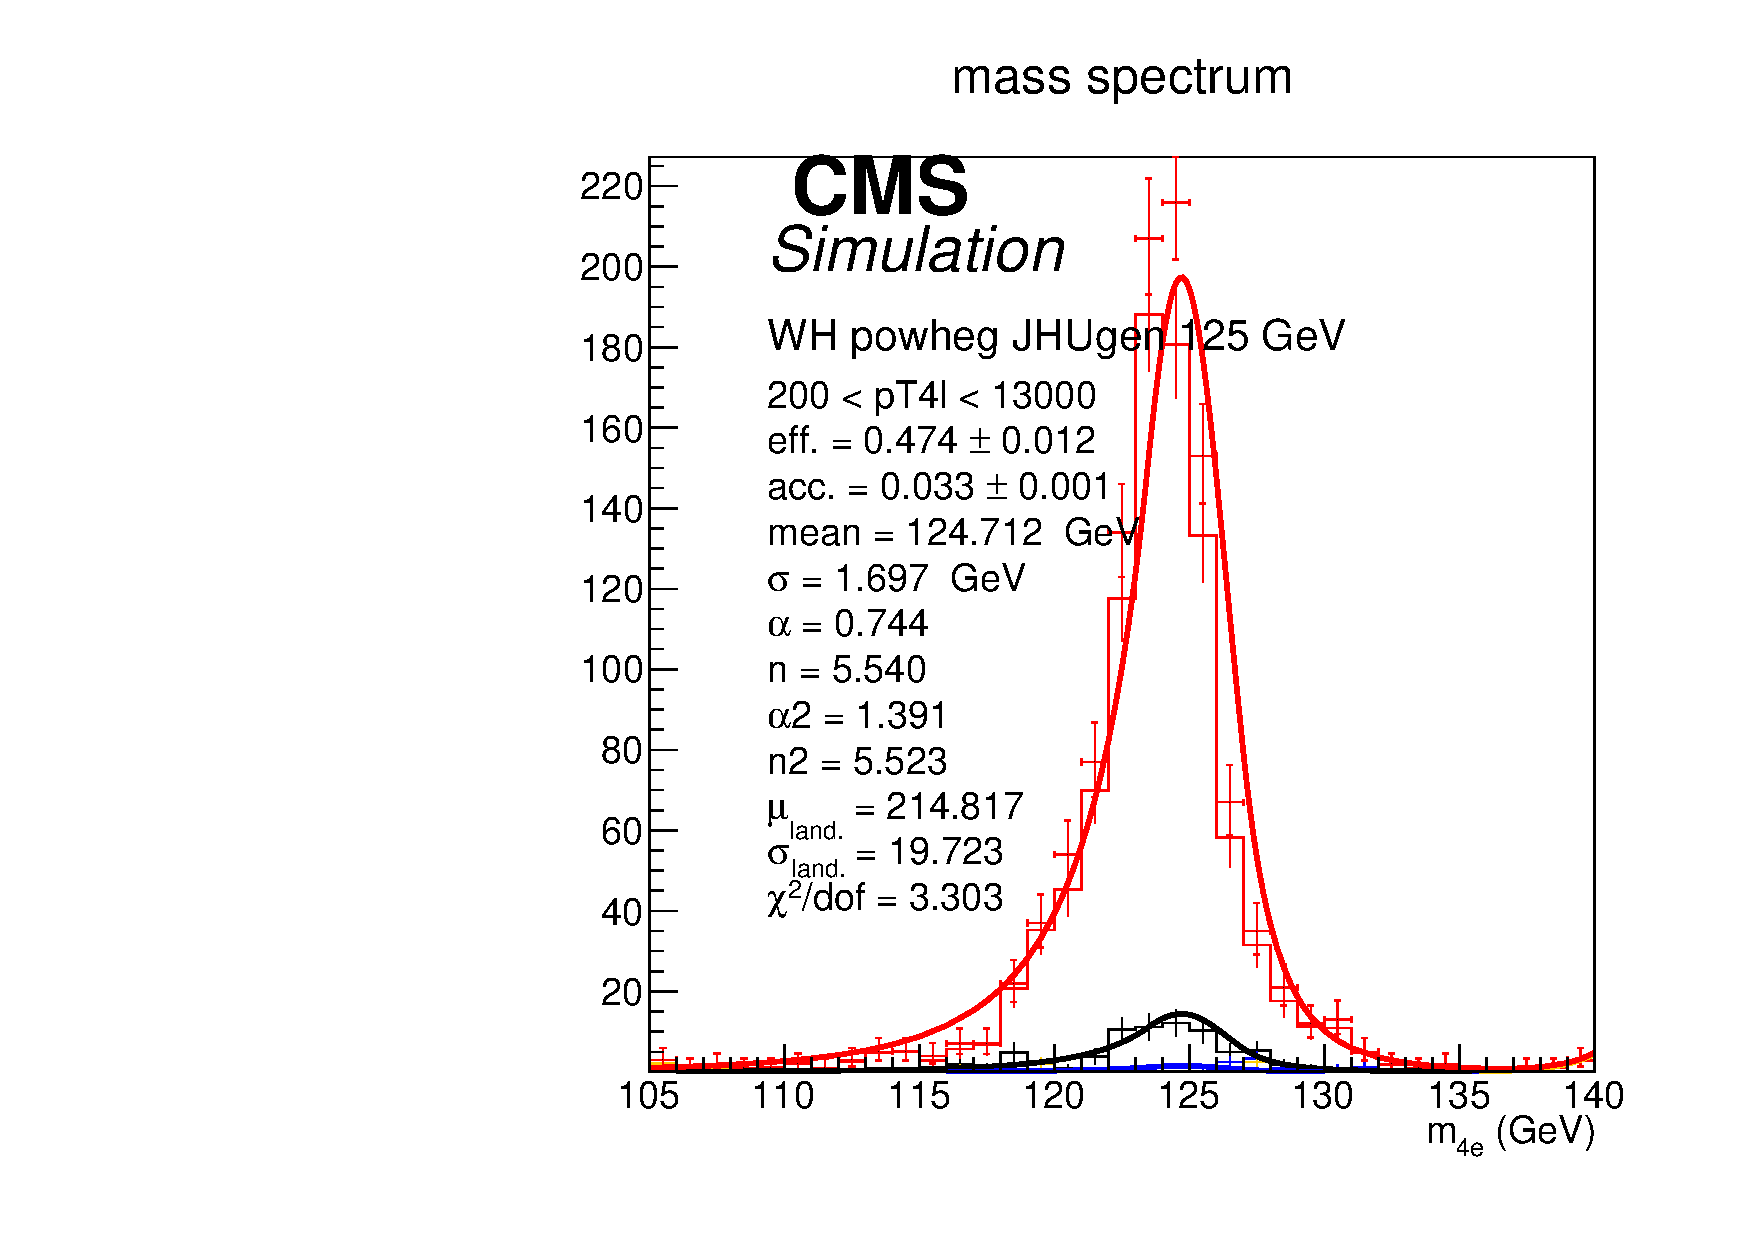
\includegraphics[width=0.3\textwidth,angle=0]{Figures/Appendix//WH_powheg_JHUgen_125_4e_pT4l_genbin6_recobin6_effs_genWeight*pileupWeight*dataMCWeight.pdf}
      \label{fig:sigfits-pT4l-WH-powheg15-JHUgen-125-maintext:g}
    }
    \\
    \caption{ Example signal shapes at reconstruction level for a resonance of m(4$\ell$) in $4e$ final state for the $WH$ production mode from {\sc powheg+JHUGen} in different bins of $\pt(\mathrm{H})$. The black curve represents events which do not pass the fiducial volume selection. The curve has no effect on the result.
    }
  \label{fig:sigfits-pT4l-WH-powheg15-JHUgen-125-maintext}
 \end{center}
\end{figure} \clearpage


\begin{figure}[htb]
  \begin{center}
    \subfigure[$0.0 < \pt(\mathrm{H}) < 15.0 $]{
      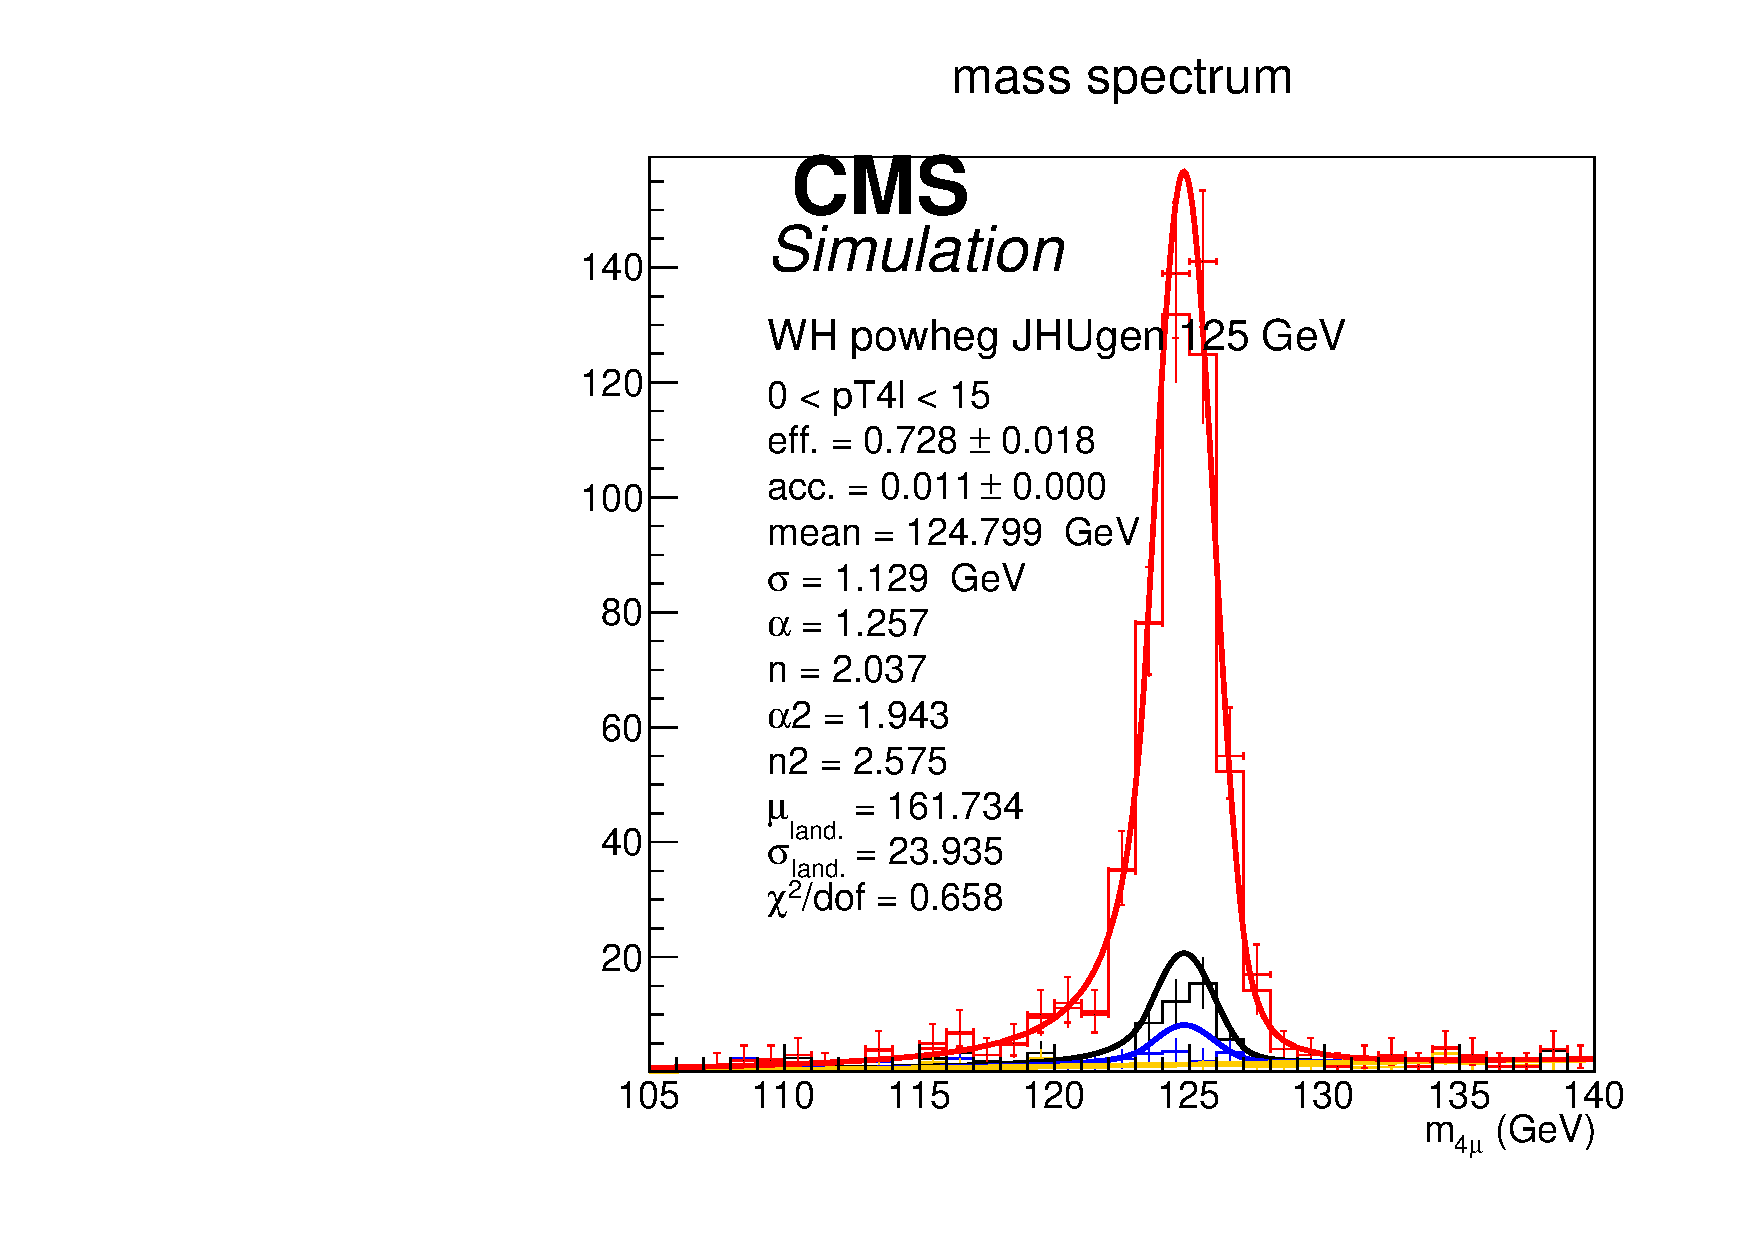
\includegraphics[width=0.3\textwidth,angle=0]{Figures/Appendix//WH_powheg_JHUgen_125_4mu_pT4l_genbin0_recobin0_effs_genWeight*pileupWeight*dataMCWeight.pdf}
      \label{fig:sigfits-pT4l-WH-powheg15-JHUgen-125-maintext:a}
    }
    \subfigure[$15.0 < \pt(\mathrm{H}) < 30.0$]{
      \includegraphics[width=0.3\textwidth,angle=0]{Figures/Appendix//WH_powheg_JHUgen_125_4mu_pT4l_genbin1_recobin1_effs_genWeight*pileupWeight*dataMCWeight.pdf}
      \label{fig:sigfits-pT4l-WH-powheg15-JHUgen-125-maintext:b}
    }
   \subfigure[$30.0 < \pt(\mathrm{H}) < 45.0$]{
      \includegraphics[width=0.3\textwidth,angle=0]{Figures/Appendix//WH_powheg_JHUgen_125_4mu_pT4l_genbin2_recobin2_effs_genWeight*pileupWeight*dataMCWeight.pdf}
      \label{fig:sigfits-pT4l-WH-powheg15-JHUgen-125-maintext:c}
    }  \\
    \subfigure[$45.0 < \pt(\mathrm{H}) < 80.0$]{
      \includegraphics[width=0.3\textwidth,angle=0]{Figures/Appendix//WH_powheg_JHUgen_125_4mu_pT4l_genbin3_recobin3_effs_genWeight*pileupWeight*dataMCWeight.pdf}
      \label{fig:sigfits-pT4l-WH-powheg15-JHUgen-125-maintext:d}
    }
    \subfigure[$80.0 < \pt(\mathrm{H}) < 120.0$]{
      \includegraphics[width=0.3\textwidth,angle=0]{Figures/Appendix//WH_powheg_JHUgen_125_4mu_pT4l_genbin4_recobin4_effs_genWeight*pileupWeight*dataMCWeight.pdf}
      \label{fig:sigfits-pT4l-WH-powheg15-JHUgen-125-maintext:e}
    }
    \subfigure[$120.0 < \pt(\mathrm{H}) < 200.0$]{
      \includegraphics[width=0.3\textwidth,angle=0]{Figures/Appendix//WH_powheg_JHUgen_125_4mu_pT4l_genbin5_recobin5_effs_genWeight*pileupWeight*dataMCWeight.pdf}
      \label{fig:sigfits-pT4l-WH-powheg15-JHUgen-125-maintext:f}
    } \\
    \subfigure[$200.0 < \pt(\mathrm{H}) < 13000.0$]{
      \includegraphics[width=0.3\textwidth,angle=0]{Figures/Appendix//WH_powheg_JHUgen_125_4mu_pT4l_genbin6_recobin6_effs_genWeight*pileupWeight*dataMCWeight.pdf}
      \label{fig:sigfits-pT4l-WH-powheg15-JHUgen-125-maintext:g}
    }
    \\
    \caption{ Example signal shapes at reconstruction level for a resonance of m(4$\ell$) in $4\mu$ final state for the $gg\rightarrow \mathrm{H}$ production mode from {\sc powheg+JHUGen} in different bins of $\pt(\mathrm{H})$. The black curve represents events which do not pass the fiducial volume selection. The curve has no effect on the result.
    }
  \label{fig:sigfits-pT4l-WH-powheg15-JHUgen-125-maintext}
 \end{center}
\end{figure} \clearpage

\begin{figure}[htb]
  \begin{center}
    \subfigure[$0.0 < \pt(\mathrm{H}) < 15.0 $]{
      \includegraphics[width=0.3\textwidth,angle=0]{Figures/Appendix//ZH_powheg_JHUgen_125_2e2mu_pT4l_genbin0_recobin0_effs_genWeight*pileupWeight*dataMCWeight.pdf}
      \label{fig:sigfits-pT4l-ZH-powheg15-JHUgen-125-maintext:a}
    }
    \subfigure[$15.0 < \pt(\mathrm{H}) < 30.0$]{
      \includegraphics[width=0.3\textwidth,angle=0]{Figures/Appendix//ZH_powheg_JHUgen_125_2e2mu_pT4l_genbin1_recobin1_effs_genWeight*pileupWeight*dataMCWeight.pdf}
      \label{fig:sigfits-pT4l-ZH-powheg15-JHUgen-125-maintext:b}
    }
   \subfigure[$30.0 < \pt(\mathrm{H}) < 45.0$]{
      \includegraphics[width=0.3\textwidth,angle=0]{Figures/Appendix//ZH_powheg_JHUgen_125_2e2mu_pT4l_genbin2_recobin2_effs_genWeight*pileupWeight*dataMCWeight.pdf}
      \label{fig:sigfits-pT4l-ZH-powheg15-JHUgen-125-maintext:c}
    }  \\
    \subfigure[$45.0 < \pt(\mathrm{H}) < 80.0$]{
      \includegraphics[width=0.3\textwidth,angle=0]{Figures/Appendix//ZH_powheg_JHUgen_125_2e2mu_pT4l_genbin3_recobin3_effs_genWeight*pileupWeight*dataMCWeight.pdf}
      \label{fig:sigfits-pT4l-ZH-powheg15-JHUgen-125-maintext:d}
    }
    \subfigure[$80.0 < \pt(\mathrm{H}) < 120.0$]{
      \includegraphics[width=0.3\textwidth,angle=0]{Figures/Appendix//ZH_powheg_JHUgen_125_2e2mu_pT4l_genbin4_recobin4_effs_genWeight*pileupWeight*dataMCWeight.pdf}
      \label{fig:sigfits-pT4l-ZH-powheg15-JHUgen-125-maintext:e}
    }
    \subfigure[$120.0 < \pt(\mathrm{H}) < 200.0$]{
      \includegraphics[width=0.3\textwidth,angle=0]{Figures/Appendix//ZH_powheg_JHUgen_125_2e2mu_pT4l_genbin5_recobin5_effs_genWeight*pileupWeight*dataMCWeight.pdf}
      \label{fig:sigfits-pT4l-ZH-powheg15-JHUgen-125-maintext:f}
    } \\
    \subfigure[$200.0 < \pt(\mathrm{H}) < 13000.0$]{
      \includegraphics[width=0.3\textwidth,angle=0]{Figures/Appendix//ZH_powheg_JHUgen_125_2e2mu_pT4l_genbin6_recobin6_effs_genWeight*pileupWeight*dataMCWeight.pdf}
      \label{fig:sigfits-pT4l-ZH-powheg15-JHUgen-125-maintext:g}
    }
    \\
    \caption{ Example signal shapes at reconstruction level for a resonance of m(4$\ell$) in $2e2\mu$ final state for the $ZH$ production mode from {\sc powheg+JHUGen} in different bins of $\pt(\mathrm{H})$. The black curve represents events which do not pass the fiducial volume selection. The curve has no effect on the result.
    }
  \label{fig:sigfits-pT4l-ZH-powheg15-JHUgen-125-maintext}
 \end{center}
\end{figure} \clearpage

\begin{figure}[htb]
  \begin{center}
    \subfigure[$0.0 < \pt(\mathrm{H}) < 15.0 $]{
      \includegraphics[width=0.3\textwidth,angle=0]{Figures/Appendix//ZH_powheg_JHUgen_125_4e_pT4l_genbin0_recobin0_effs_genWeight*pileupWeight*dataMCWeight.pdf}
      \label{fig:sigfits-pT4l-ZH-powheg15-JHUgen-125-maintext:a}
    }
    \subfigure[$15.0 < \pt(\mathrm{H}) < 30.0$]{
      \includegraphics[width=0.3\textwidth,angle=0]{Figures/Appendix//ZH_powheg_JHUgen_125_4e_pT4l_genbin1_recobin1_effs_genWeight*pileupWeight*dataMCWeight.pdf}
      \label{fig:sigfits-pT4l-ZH-powheg15-JHUgen-125-maintext:b}
    }
   \subfigure[$30.0 < \pt(\mathrm{H}) < 45.0$]{
      \includegraphics[width=0.3\textwidth,angle=0]{Figures/Appendix//ZH_powheg_JHUgen_125_4e_pT4l_genbin2_recobin2_effs_genWeight*pileupWeight*dataMCWeight.pdf}
      \label{fig:sigfits-pT4l-ZH-powheg15-JHUgen-125-maintext:c}
    }  \\
    \subfigure[$45.0 < \pt(\mathrm{H}) < 80.0$]{
      \includegraphics[width=0.3\textwidth,angle=0]{Figures/Appendix//ZH_powheg_JHUgen_125_4e_pT4l_genbin3_recobin3_effs_genWeight*pileupWeight*dataMCWeight.pdf}
      \label{fig:sigfits-pT4l-ZH-powheg15-JHUgen-125-maintext:d}
    }
    \subfigure[$80.0 < \pt(\mathrm{H}) < 120.0$]{
      \includegraphics[width=0.3\textwidth,angle=0]{Figures/Appendix//ZH_powheg_JHUgen_125_4e_pT4l_genbin4_recobin4_effs_genWeight*pileupWeight*dataMCWeight.pdf}
      \label{fig:sigfits-pT4l-ZH-powheg15-JHUgen-125-maintext:e}
    }
    \subfigure[$120.0 < \pt(\mathrm{H}) < 200.0$]{
      \includegraphics[width=0.3\textwidth,angle=0]{Figures/Appendix//ZH_powheg_JHUgen_125_4e_pT4l_genbin5_recobin5_effs_genWeight*pileupWeight*dataMCWeight.pdf}
      \label{fig:sigfits-pT4l-ZH-powheg15-JHUgen-125-maintext:f}
    } \\
    \subfigure[$200.0 < \pt(\mathrm{H}) < 13000.0$]{
      \includegraphics[width=0.3\textwidth,angle=0]{Figures/Appendix//ZH_powheg_JHUgen_125_4e_pT4l_genbin6_recobin6_effs_genWeight*pileupWeight*dataMCWeight.pdf}
      \label{fig:sigfits-pT4l-ZH-powheg15-JHUgen-125-maintext:g}
    }
    \\
    \caption{ Example signal shapes at reconstruction level for a resonance of m(4$\ell$) in $4e$ final state for the $ZH$ production mode from {\sc powheg+JHUGen} in different bins of $\pt(\mathrm{H})$. The black curve represents events which do not pass the fiducial volume selection. The curve has no effect on the result.
    }
  \label{fig:sigfits-pT4l-ZH-powheg15-JHUgen-125-maintext}
 \end{center}
\end{figure} \clearpage

\begin{figure}[htb]
  \begin{center}
    \subfigure[$0.0 < \pt(\mathrm{H}) < 15.0 $]{
      \includegraphics[width=0.3\textwidth,angle=0]{Figures/Appendix//ZH_powheg_JHUgen_125_4mu_pT4l_genbin0_recobin0_effs_genWeight*pileupWeight*dataMCWeight.pdf}
      \label{fig:sigfits-pT4l-ZH-powheg15-JHUgen-125-maintext:a}
    }
    \subfigure[$15.0 < \pt(\mathrm{H}) < 30.0$]{
      \includegraphics[width=0.3\textwidth,angle=0]{Figures/Appendix//ZH_powheg_JHUgen_125_4mu_pT4l_genbin1_recobin1_effs_genWeight*pileupWeight*dataMCWeight.pdf}
      \label{fig:sigfits-pT4l-ZH-powheg15-JHUgen-125-maintext:b}
    }
   \subfigure[$30.0 < \pt(\mathrm{H}) < 45.0$]{
      \includegraphics[width=0.3\textwidth,angle=0]{Figures/Appendix//ZH_powheg_JHUgen_125_4mu_pT4l_genbin2_recobin2_effs_genWeight*pileupWeight*dataMCWeight.pdf}
      \label{fig:sigfits-pT4l-ZH-powheg15-JHUgen-125-maintext:c}
    }  \\
    \subfigure[$45.0 < \pt(\mathrm{H}) < 80.0$]{
      \includegraphics[width=0.3\textwidth,angle=0]{Figures/Appendix//ZH_powheg_JHUgen_125_4mu_pT4l_genbin3_recobin3_effs_genWeight*pileupWeight*dataMCWeight.pdf}
      \label{fig:sigfits-pT4l-ZH-powheg15-JHUgen-125-maintext:d}
    }
    \subfigure[$80.0 < \pt(\mathrm{H}) < 120.0$]{
      \includegraphics[width=0.3\textwidth,angle=0]{Figures/Appendix//ZH_powheg_JHUgen_125_4mu_pT4l_genbin4_recobin4_effs_genWeight*pileupWeight*dataMCWeight.pdf}
      \label{fig:sigfits-pT4l-ZH-powheg15-JHUgen-125-maintext:e}
    }
    \subfigure[$120.0 < \pt(\mathrm{H}) < 200.0$]{
      \includegraphics[width=0.3\textwidth,angle=0]{Figures/Appendix//ZH_powheg_JHUgen_125_4mu_pT4l_genbin5_recobin5_effs_genWeight*pileupWeight*dataMCWeight.pdf}
      \label{fig:sigfits-pT4l-ZH-powheg15-JHUgen-125-maintext:f}
    } \\
    \subfigure[$200.0 < \pt(\mathrm{H}) < 13000.0$]{
      \includegraphics[width=0.3\textwidth,angle=0]{Figures/Appendix//ZH_powheg_JHUgen_125_4mu_pT4l_genbin6_recobin6_effs_genWeight*pileupWeight*dataMCWeight.pdf}
      \label{fig:sigfits-pT4l-ZH-powheg15-JHUgen-125-maintext:g}
    }
    \\
    \caption{ Example signal shapes at reconstruction level for a resonance of m(4$\ell$) in $4\mu$ final state for the $ZH$ production mode from {\sc powheg+JHUGen} in different bins of $\pt(\mathrm{H})$. The black curve represents events which do not pass the fiducial volume selection. The curve has no effect on the result.
    }
  \label{fig:sigfits-pT4l-ZH-powheg15-JHUgen-125-maintext}
 \end{center}
\end{figure} \clearpage

%%%%%%%%%%%%%%%%%%%%%%%%%%%%%%%%%%%%%%%%%%%%%%%%%%%%  ttH
\begin{figure}[htb]
  \begin{center}
    \subfigure[$0.0 < \pt(\mathrm{H}) < 15.0 $]{
      \includegraphics[width=0.3\textwidth,angle=0]{Figures/Appendix//ttH_powheg_JHUgen_125_2e2mu_pT4l_genbin0_recobin0_effs_genWeight*pileupWeight*dataMCWeight.pdf}
      \label{fig:sigfits-pT4l-ttH-powheg15-JHUgen-125-maintext:a}
    }
    \subfigure[$15.0 < \pt(\mathrm{H}) < 30.0$]{
      \includegraphics[width=0.3\textwidth,angle=0]{Figures/Appendix//ttH_powheg_JHUgen_125_2e2mu_pT4l_genbin1_recobin1_effs_genWeight*pileupWeight*dataMCWeight.pdf}
      \label{fig:sigfits-pT4l-ttH-powheg15-JHUgen-125-maintext:b}
    }
   \subfigure[$30.0 < \pt(\mathrm{H}) < 45.0$]{
      \includegraphics[width=0.3\textwidth,angle=0]{Figures/Appendix//ttH_powheg_JHUgen_125_2e2mu_pT4l_genbin2_recobin2_effs_genWeight*pileupWeight*dataMCWeight.pdf}
      \label{fig:sigfits-pT4l-ttH-powheg15-JHUgen-125-maintext:c}
    }  \\
    \subfigure[$45.0 < \pt(\mathrm{H}) < 80.0$]{
      \includegraphics[width=0.3\textwidth,angle=0]{Figures/Appendix//ttH_powheg_JHUgen_125_2e2mu_pT4l_genbin3_recobin3_effs_genWeight*pileupWeight*dataMCWeight.pdf}
      \label{fig:sigfits-pT4l-ttH-powheg15-JHUgen-125-maintext:d}
    }
    \subfigure[$80.0 < \pt(\mathrm{H}) < 120.0$]{
      \includegraphics[width=0.3\textwidth,angle=0]{Figures/Appendix//ttH_powheg_JHUgen_125_2e2mu_pT4l_genbin4_recobin4_effs_genWeight*pileupWeight*dataMCWeight.pdf}
      \label{fig:sigfits-pT4l-ttH-powheg15-JHUgen-125-maintext:e}
    }
    \subfigure[$120.0 < \pt(\mathrm{H}) < 200.0$]{
      \includegraphics[width=0.3\textwidth,angle=0]{Figures/Appendix//ttH_powheg_JHUgen_125_2e2mu_pT4l_genbin5_recobin5_effs_genWeight*pileupWeight*dataMCWeight.pdf}
      \label{fig:sigfits-pT4l-ttH-powheg15-JHUgen-125-maintext:f}
    } \\
    \subfigure[$200.0 < \pt(\mathrm{H}) < 13000.0$]{
      \includegraphics[width=0.3\textwidth,angle=0]{Figures/Appendix//ttH_powheg_JHUgen_125_2e2mu_pT4l_genbin6_recobin6_effs_genWeight*pileupWeight*dataMCWeight.pdf}
      \label{fig:sigfits-pT4l-ttH-powheg15-JHUgen-125-maintext:g}
    }
    \\
    \caption{ Example signal shapes at reconstruction level for a resonance of m(4$\ell$) in $2e2\mu$ final state for the $ttH$ production mode from {\sc powheg+JHUGen} in different bins of $\pt(\mathrm{H})$. The black curve represents events which do not pass the fiducial volume selection. The curve has no effect on the result.
    }
  \label{fig:sigfits-pT4l-ttH-powheg15-JHUgen-125-maintext}
 \end{center}
\end{figure} \clearpage

\begin{figure}[htb]
  \begin{center}
    \subfigure[$0.0 < \pt(\mathrm{H}) < 15.0 $]{
      \includegraphics[width=0.3\textwidth,angle=0]{Figures/Appendix//ggH_powheg_JHUgen_125_4e_pT4l_genbin0_recobin0_effs_genWeight*pileupWeight*dataMCWeight.pdf}
      \label{fig:sigfits-pT4l-ggH-powheg15-JHUgen-125-maintext:a}
    }
    \subfigure[$15.0 < \pt(\mathrm{H}) < 30.0$]{
      \includegraphics[width=0.3\textwidth,angle=0]{Figures/Appendix//ggH_powheg_JHUgen_125_4e_pT4l_genbin1_recobin1_effs_genWeight*pileupWeight*dataMCWeight.pdf}
      \label{fig:sigfits-pT4l-ggH-powheg15-JHUgen-125-maintext:b}
    }
   \subfigure[$30.0 < \pt(\mathrm{H}) < 45.0$]{
      \includegraphics[width=0.3\textwidth,angle=0]{Figures/Appendix//ggH_powheg_JHUgen_125_4e_pT4l_genbin2_recobin2_effs_genWeight*pileupWeight*dataMCWeight.pdf}
      \label{fig:sigfits-pT4l-ggH-powheg15-JHUgen-125-maintext:c}
    }  \\
    \subfigure[$45.0 < \pt(\mathrm{H}) < 80.0$]{
      \includegraphics[width=0.3\textwidth,angle=0]{Figures/Appendix//ggH_powheg_JHUgen_125_4e_pT4l_genbin3_recobin3_effs_genWeight*pileupWeight*dataMCWeight.pdf}
      \label{fig:sigfits-pT4l-ggH-powheg15-JHUgen-125-maintext:d}
    }
    \subfigure[$80.0 < \pt(\mathrm{H}) < 120.0$]{
      \includegraphics[width=0.3\textwidth,angle=0]{Figures/Appendix//ggH_powheg_JHUgen_125_4e_pT4l_genbin4_recobin4_effs_genWeight*pileupWeight*dataMCWeight.pdf}
      \label{fig:sigfits-pT4l-ggH-powheg15-JHUgen-125-maintext:e}
    }
    \subfigure[$120.0 < \pt(\mathrm{H}) < 200.0$]{
      \includegraphics[width=0.3\textwidth,angle=0]{Figures/Appendix//ggH_powheg_JHUgen_125_4e_pT4l_genbin5_recobin5_effs_genWeight*pileupWeight*dataMCWeight.pdf}
      \label{fig:sigfits-pT4l-ggH-powheg15-JHUgen-125-maintext:f}
    } \\
    \subfigure[$200.0 < \pt(\mathrm{H}) < 13000.0$]{
      \includegraphics[width=0.3\textwidth,angle=0]{Figures/Appendix//ggH_powheg_JHUgen_125_4e_pT4l_genbin6_recobin6_effs_genWeight*pileupWeight*dataMCWeight.pdf}
      \label{fig:sigfits-pT4l-ggH-powheg15-JHUgen-125-maintext:g}
    }
    \\
    \caption{ Example signal shapes at reconstruction level for a resonance of m(4$\ell$) in $4e$ final state for the $ttH$ production mode from {\sc powheg+JHUGen} in different bins of $\pt(\mathrm{H})$. The black curve represents events which do not pass the fiducial volume selection. The curve has no effect on the result.
    }
  \label{fig:sigfits-pT4l-ggH-powheg15-JHUgen-125-maintext}
 \end{center}
\end{figure} \clearpage



\begin{figure}[htb]
  \begin{center}
    \subfigure[$0.0 < \pt(\mathrm{H}) < 15.0 $]{
      \includegraphics[width=0.3\textwidth,angle=0]{Figures/Appendix//ttH_powheg_JHUgen_125_4mu_pT4l_genbin0_recobin0_effs_genWeight*pileupWeight*dataMCWeight.pdf}
      \label{fig:sigfits-pT4l-ttH-powheg15-JHUgen-125-maintext:a}
    }
    \subfigure[$15.0 < \pt(\mathrm{H}) < 30.0$]{
      \includegraphics[width=0.3\textwidth,angle=0]{Figures/Appendix//ttH_powheg_JHUgen_125_4mu_pT4l_genbin1_recobin1_effs_genWeight*pileupWeight*dataMCWeight.pdf}
      \label{fig:sigfits-pT4l-ttH-powheg15-JHUgen-125-maintext:b}
    }
   \subfigure[$30.0 < \pt(\mathrm{H}) < 45.0$]{
      \includegraphics[width=0.3\textwidth,angle=0]{Figures/Appendix//ttH_powheg_JHUgen_125_4mu_pT4l_genbin2_recobin2_effs_genWeight*pileupWeight*dataMCWeight.pdf}
      \label{fig:sigfits-pT4l-ttH-powheg15-JHUgen-125-maintext:c}
    }  \\
    \subfigure[$45.0 < \pt(\mathrm{H}) < 80.0$]{
      \includegraphics[width=0.3\textwidth,angle=0]{Figures/Appendix//ttH_powheg_JHUgen_125_4mu_pT4l_genbin3_recobin3_effs_genWeight*pileupWeight*dataMCWeight.pdf}
      \label{fig:sigfits-pT4l-ttH-powheg15-JHUgen-125-maintext:d}
    }
    \subfigure[$80.0 < \pt(\mathrm{H}) < 120.0$]{
      \includegraphics[width=0.3\textwidth,angle=0]{Figures/Appendix//ttH_powheg_JHUgen_125_4mu_pT4l_genbin4_recobin4_effs_genWeight*pileupWeight*dataMCWeight.pdf}
      \label{fig:sigfits-pT4l-ttH-powheg15-JHUgen-125-maintext:e}
    }
    \subfigure[$120.0 < \pt(\mathrm{H}) < 200.0$]{
      \includegraphics[width=0.3\textwidth,angle=0]{Figures/Appendix//ttH_powheg_JHUgen_125_4mu_pT4l_genbin5_recobin5_effs_genWeight*pileupWeight*dataMCWeight.pdf}
      \label{fig:sigfits-pT4l-ttH-powheg15-JHUgen-125-maintext:f}
    } \\
    \subfigure[$200.0 < \pt(\mathrm{H}) < 13000.0$]{
      \includegraphics[width=0.3\textwidth,angle=0]{Figures/Appendix//ttH_powheg_JHUgen_125_4mu_pT4l_genbin6_recobin6_effs_genWeight*pileupWeight*dataMCWeight.pdf}
      \label{fig:sigfits-pT4l-ttH-powheg15-JHUgen-125-maintext:g}
    }
    \\
    \caption{ Example signal shapes at reconstruction level for a resonance of m(4$\ell$) in $4\mu$ final state for the $ttH$ production mode from {\sc powheg+JHUGen} in different bins of $\pt(\mathrm{H})$. The black curve represents events which do not pass the fiducial volume selection. The curve has no effect on the result.
    }
  \label{fig:sigfits-pT4l-ttH-powheg15-JHUgen-125-maintext}
 \end{center}
\end{figure} \clearpage


%%%%%%%%%%%%%%%%%%%%%%%%%%%%%  2D response matrices

\begin{figure}[!h!tb]
  \begin{center}
    \subfigure[$gg\rightarrow$H ({\sc powheg+JHUgen})]{
    \includegraphics[width=0.30\textwidth,angle=0]{Figures/Appendix//eff2d_ggH_powheg_JHUgen_125_pT4l_4e.pdf}
    \label{fig:eff-pT4l-4e:a}
    }
%    \subfigure[$gg\rightarrow$H ({\sc minloHJJ})]{
%    \includegraphics[width=0.30\textwidth,angle=0]{Figures/Appendix//eff2d_ggH_minloHJJ_125_pT4l_4e.pdf}
%    \label{fig:eff-pT4l-4e:b}
%    } \\
    \subfigure[VBF ({\sc powheg})]{
    \includegraphics[width=0.30\textwidth,angle=0]{Figures/Appendix//eff2d_VBF_powheg_JHUgen_125_pT4l_4e.pdf}
    \label{fig:eff-pT4l-4e:c}
    }
    \subfigure[WH ({\sc pythia})]{
    \includegraphics[width=0.30\textwidth,angle=0]{Figures/Appendix//eff2d_WH_powheg_JHUgen_125_pT4l_4e.pdf}
    \label{fig:eff-pT4l-4e:d}
    } \\
    \subfigure[ZH ({\sc pythia})]{
    \includegraphics[width=0.30\textwidth,angle=0]{Figures/Appendix//eff2d_ZH_powheg_JHUgen_125_pT4l_4e.pdf}
    \label{fig:eff-pT4l-4e:e}
    }
    \subfigure[ttH ({\sc pythia})]{
    \includegraphics[width=0.30\textwidth,angle=0]{Figures/Appendix//eff2d_ttH_powheg_JHUgen_125_pT4l_4e.pdf}
    \label{fig:eff-pT4l-4e:f}
    } 
    \caption{ Efficiency matrices for  $\pt({\rm H})$ for different SM production modes in the $4e$ final state. }
    \label{fig:eff-pT4l-4e}
  \end{center}
\end{figure} \clearpage


\begin{figure}[!h!tb]
  \begin{center}
    \subfigure[$gg\rightarrow$H ({\sc powheg+JHUgen})]{
    \includegraphics[width=0.30\textwidth,angle=0]{Figures/Appendix//eff2d_ggH_powheg_JHUgen_125_pT4l_4mu.pdf}
    \label{fig:eff-pT4l-4mu:a}
    }
%    \subfigure[$\Pg\Pg\rightarrow$H ({\sc minloHJJ})]{
%    \includegraphics[width=0.30\textwidth,angle=0]{Figures/Appendix//eff2d_ggH_minloHJJ_125_pT4l_4mu.pdf}
%    \label{fig:eff-pT4l-4mu:b}
%    } \\
    \subfigure[VBF ({\sc powheg})]{
    \includegraphics[width=0.30\textwidth,angle=0]{Figures/Appendix//eff2d_VBF_powheg_JHUgen_125_pT4l_4mu.pdf}
    \label{fig:eff-pT4l-4mu:c}
    }
    \subfigure[WH ({\sc pythia})]{
    \includegraphics[width=0.30\textwidth,angle=0]{Figures/Appendix//eff2d_WH_powheg_JHUgen_125_pT4l_4mu.pdf}
    \label{fig:eff-pT4l-4mu:d}
    } \\
    \subfigure[ZH ({\sc pythia})]{
    \includegraphics[width=0.30\textwidth,angle=0]{Figures/Appendix//eff2d_ZH_powheg_JHUgen_125_pT4l_4mu.pdf}
    \label{fig:eff-pT4l-4mu:e}
    }
    \subfigure[ttH ({\sc pythia})]{
    \includegraphics[width=0.30\textwidth,angle=0]{Figures/Appendix//eff2d_ttH_powheg_JHUgen_125_pT4l_4mu.pdf}
    \label{fig:eff-pT4l-4mu:f}
    } 
    \caption{ Efficiency matrices for  $\pt({\rm H})$ for different SM production modes in the $4\mu$ final state. }
    \label{fig:eff-pT4l-4mu}
  \end{center}
\end{figure} \clearpage

\begin{figure}[!h!tb]
  \begin{center}
    \subfigure[$gg\rightarrow$H ({\sc powheg+JHUgen})]{
    \includegraphics[width=0.30\textwidth,angle=0]{Figures/Appendix//eff2d_ggH_powheg_JHUgen_125_pT4l_2e2mu.pdf}
    \label{fig:eff-pT4l-2e2mu:a}
    }
%    \subfigure[$\Pg\Pg\rightarrow$H ({\sc minloHJJ})]{
%    \includegraphics[width=0.30\textwidth,angle=0]{Figures/Appendix//eff2d_ggH_minloHJJ_125_pT4l_2e2mu.pdf}
%    \label{fig:eff-pT4l-2e2mu:b}
%    } \\
    \subfigure[VBF ({\sc powheg})]{
    \includegraphics[width=0.30\textwidth,angle=0]{Figures/Appendix//eff2d_VBF_powheg_JHUgen_125_pT4l_2e2mu.pdf}
    \label{fig:eff-pT4l-2e2mu:c}
    }
    \subfigure[WH ({\sc pythia})]{
    \includegraphics[width=0.30\textwidth,angle=0]{Figures/Appendix//eff2d_WH_powheg_JHUgen_125_pT4l_2e2mu.pdf}
    \label{fig:eff-pT4l-2e2mu:d}
    } \\
    \subfigure[ZH ({\sc pythia})]{
    \includegraphics[width=0.30\textwidth,angle=0]{Figures/Appendix//eff2d_ZH_powheg_JHUgen_125_pT4l_2e2mu.pdf}
    \label{fig:eff-pT4l-2e2mu:e}
    }
    \subfigure[ttH ({\sc pythia})]{
    \includegraphics[width=0.30\textwidth,angle=0]{Figures/Appendix//eff2d_ttH_powheg_JHUgen_125_pT4l_2e2mu.pdf}
    \label{fig:eff-pT4l-2e2mu:f}
    } 
    \caption{ Efficiency matrices for $\pt({\rm H})$ for different SM production modes in the $2e2\mu$ final state. }
    \label{fig:eff-pT4l-2e2mu}
  \end{center}
\end{figure} \clearpage


\subsection[Differential bins - rapidity of the Higgs boson]{Signal inputs in different bins of $|y(\mathrm{H})|$ }

\begin{figure}[!h!tb]
  \begin{center}
    \subfigure[$gg\rightarrow$H ({\sc powheg+JHUgen})]{
    \includegraphics[width=0.30\textwidth,angle=0]{Figures/Appendix//eff2d_ggH_powheg_JHUgen_125_rapidity4l_4e.pdf}
    \label{fig:eff-rapidity4l-4e:a}
    }
%    \subfigure[$\Pg\Pg\rightarrow$H ({\sc minloHJJ})]{
%    \includegraphics[width=0.30\textwidth,angle=0]{Figures/Appendix//eff2d_ggH_minloHJJ_125_rapidity4l_4e.pdf}
%    \label{fig:eff-rapidity4l-4e:b}
%    } \\
    \subfigure[VBF ({\sc powheg})]{
    \includegraphics[width=0.30\textwidth,angle=0]{Figures/Appendix//eff2d_VBF_powheg_JHUgen_125_rapidity4l_4e.pdf}
    \label{fig:eff-rapidity4l-4e:c}
    }
    \subfigure[WH ({\sc pythia})]{
    \includegraphics[width=0.30\textwidth,angle=0]{Figures/Appendix//eff2d_WH_powheg_JHUgen_125_rapidity4l_4e.pdf}
    \label{fig:eff-rapidity4l-4e:d}
    } \\
    \subfigure[ZH ({\sc pythia})]{
    \includegraphics[width=0.30\textwidth,angle=0]{Figures/Appendix//eff2d_ZH_powheg_JHUgen_125_rapidity4l_4e.pdf}
    \label{fig:eff-rapidity4l-4e:e}
    }
    \subfigure[ttH ({\sc pythia})]{
    \includegraphics[width=0.30\textwidth,angle=0]{Figures/Appendix//eff2d_ttH_powheg_JHUgen_125_rapidity4l_4e.pdf}
    \label{fig:eff-rapidity4l-4e:f}
    } 
    \caption{ Efficiency matrices for $|y({\rm H})|$ for different SM production modes in the $4e$ final state. }
    \label{fig:eff-rapidity4l-4e}
  \end{center}
\end{figure} \clearpage


\begin{figure}[!h!tb]
  \begin{center}
    \subfigure[$gg\rightarrow$H ({\sc powheg+JHUgen})]{
    \includegraphics[width=0.30\textwidth,angle=0]{Figures/Appendix//eff2d_ggH_powheg_JHUgen_125_rapidity4l_4mu.pdf}
    \label{fig:eff-rapidity4l-4mu:a}
    }
%    \subfigure[$\Pg\Pg\rightarrow$H ({\sc minloHJJ})]{
%    \includegraphics[width=0.30\textwidth,angle=0]{Figures/Appendix//eff2d_ggH_minloHJJ_125_rapidity4l_4mu.pdf}
%    \label{fig:eff-rapidity4l-4mu:b}
%    } \\
    \subfigure[VBF ({\sc powheg})]{
    \includegraphics[width=0.30\textwidth,angle=0]{Figures/Appendix//eff2d_VBF_powheg_JHUgen_125_rapidity4l_4mu.pdf}
    \label{fig:eff-rapidity4l-4mu:c}
    }
    \subfigure[WH ({\sc pythia})]{
    \includegraphics[width=0.30\textwidth,angle=0]{Figures/Appendix//eff2d_WH_powheg_JHUgen_125_rapidity4l_4mu.pdf}
    \label{fig:eff-rapidity4l-4mu:d}
    } \\
    \subfigure[ZH ({\sc pythia})]{
    \includegraphics[width=0.30\textwidth,angle=0]{Figures/Appendix//eff2d_ZH_powheg_JHUgen_125_rapidity4l_4mu.pdf}
    \label{fig:eff-rapidity4l-4mu:e}
    }
    \subfigure[ttH ({\sc pythia})]{
    \includegraphics[width=0.30\textwidth,angle=0]{Figures/Appendix//eff2d_ttH_powheg_JHUgen_125_rapidity4l_4mu.pdf}
    \label{fig:eff-rapidity4l-4mu:f}
    } 
    \caption{ Efficiency matrices for $|y({\rm H})|$ for different SM production modes in the $4\mu$ final state. }
    \label{fig:eff-rapidity4l-4mu}
  \end{center}
\end{figure} \clearpage

\begin{figure}[!h!tb]
  \begin{center}
    \subfigure[$gg\rightarrow$H ({\sc powheg+JHUgen})]{
    \includegraphics[width=0.30\textwidth,angle=0]{Figures/Appendix//eff2d_ggH_powheg_JHUgen_125_rapidity4l_2e2mu.pdf}
    \label{fig:eff-rapidity4l-2e2mu:a}
    }
%    \subfigure[$\Pg\Pg\rightarrow$H ({\sc minloHJJ})]{
%    \includegraphics[width=0.30\textwidth,angle=0]{Figures/Appendix//eff2d_ggH_minloHJJ_125_rapidity4l_2e2mu.pdf}
%    \label{fig:eff-rapidity4l-2e2mu:b}
%    } \\
    \subfigure[VBF ({\sc powheg})]{
    \includegraphics[width=0.30\textwidth,angle=0]{Figures/Appendix//eff2d_VBF_powheg_JHUgen_125_rapidity4l_2e2mu.pdf}
    \label{fig:eff-rapidity4l-2e2mu:c}
    }
    \subfigure[WH ({\sc pythia})]{
    \includegraphics[width=0.30\textwidth,angle=0]{Figures/Appendix//eff2d_WH_powheg_JHUgen_125_rapidity4l_2e2mu.pdf}
    \label{fig:eff-rapidity4l-2e2mu:d}
    } \\
    \subfigure[ZH ({\sc pythia})]{
    \includegraphics[width=0.30\textwidth,angle=0]{Figures/Appendix//eff2d_ZH_powheg_JHUgen_125_rapidity4l_2e2mu.pdf}
    \label{fig:eff-rapidity4l-2e2mu:e}
    }
    \subfigure[ttH ({\sc pythia})]{
    \includegraphics[width=0.30\textwidth,angle=0]{Figures/Appendix//eff2d_ttH_powheg_JHUgen_125_rapidity4l_2e2mu.pdf}
    \label{fig:eff-rapidity4l-2e2mu:f}
    } 
    \caption{ Efficiency matrices for $|y({\rm H})|$ for different SM production modes in the $2e2\mu$ final state. }
    \label{fig:eff-rapidity4l-2e2mu}
  \end{center}
\end{figure} \clearpage

%%%%%%%%%%%%%%%%%%%%%%%%%%%%%%% njets
\subsection[Signal fits in differential bins - number of jets]{Fits in different bins of N(jets) }


\begin{figure}[!h!tb]
  \begin{center}
    \subfigure[$gg\rightarrow$H ({\sc powheg+JHUgen})]{
    \includegraphics[width=0.30\textwidth,angle=0]{Figures/Appendix//eff2d_ggH_powheg_JHUgen_125_njets_pt30_eta2p5_4e.pdf}
    \label{fig:eff-njets_pt30_eta2p5-4e:a}
    }
%    \subfigure[$\Pg\Pg\rightarrow$H ({\sc minloHJJ})]{
%    \includegraphics[width=0.30\textwidth,angle=0]{Figures/Appendix//eff2d_ggH_minloHJJ_125_njets_pt30_eta2p5_4e.pdf}
%    \label{fig:eff-njets_pt30_eta2p5-4e:b}
%    } \\
    \subfigure[VBF ({\sc powheg})]{
    \includegraphics[width=0.30\textwidth,angle=0]{Figures/Appendix//eff2d_VBF_powheg_JHUgen_125_njets_pt30_eta2p5_4e.pdf}
    \label{fig:eff-njets_pt30_eta2p5-4e:c}
    }
    \subfigure[WH ({\sc pythia})]{
    \includegraphics[width=0.30\textwidth,angle=0]{Figures/Appendix//eff2d_WH_powheg_JHUgen_125_njets_pt30_eta2p5_4e.pdf}
    \label{fig:eff-njets_pt30_eta2p5-4e:d}
    } \\
    \subfigure[ZH ({\sc pythia})]{
    \includegraphics[width=0.30\textwidth,angle=0]{Figures/Appendix//eff2d_ZH_powheg_JHUgen_125_njets_pt30_eta2p5_4e.pdf}
    \label{fig:eff-njets_pt30_eta2p5-4e:e}
    }
    \subfigure[ttH ({\sc pythia})]{
    \includegraphics[width=0.30\textwidth,angle=0]{Figures/Appendix//eff2d_ttH_powheg_JHUgen_125_njets_pt30_eta2p5_4e.pdf}
    \label{fig:eff-njets_pt30_eta2p5-4e:f}
    } 
    \caption{ Efficiency matrices for N(jets) for different SM production modes in the $4e$ final state. }
    \label{fig:eff-njets_pt30_eta2p5-4e}
  \end{center}
\end{figure} \clearpage


\begin{figure}[!h!tb]
  \begin{center}
    \subfigure[$gg\rightarrow$H ({\sc powheg+JHUgen})]{
    \includegraphics[width=0.30\textwidth,angle=0]{Figures/Appendix//eff2d_ggH_powheg_JHUgen_125_njets_pt30_eta2p5_4mu.pdf}
    \label{fig:eff-njets_pt30_eta2p5-4mu:a}
    }
%    \subfigure[$\Pg\Pg\rightarrow$H ({\sc minloHJJ})]{
%    \includegraphics[width=0.30\textwidth,angle=0]{Figures/Appendix//eff2d_ggH_minloHJJ_125_njets_pt30_eta2p5_4mu.pdf}
%    \label{fig:eff-njets_pt30_eta2p5-4mu:b}
%    } \\
    \subfigure[VBF ({\sc powheg})]{
    \includegraphics[width=0.30\textwidth,angle=0]{Figures/Appendix//eff2d_VBF_powheg_JHUgen_125_njets_pt30_eta2p5_4mu.pdf}
    \label{fig:eff-njets_pt30_eta2p5-4mu:c}
    }
    \subfigure[WH ({\sc pythia})]{
    \includegraphics[width=0.30\textwidth,angle=0]{Figures/Appendix//eff2d_WH_powheg_JHUgen_125_njets_pt30_eta2p5_4mu.pdf}
    \label{fig:eff-njets_pt30_eta2p5-4mu:d}
    } \\
    \subfigure[ZH ({\sc pythia})]{
    \includegraphics[width=0.30\textwidth,angle=0]{Figures/Appendix//eff2d_ZH_powheg_JHUgen_125_njets_pt30_eta2p5_4mu.pdf}
    \label{fig:eff-njets_pt30_eta2p5-4mu:e}
    }
    \subfigure[ttH ({\sc pythia})]{
    \includegraphics[width=0.30\textwidth,angle=0]{Figures/Appendix//eff2d_ttH_powheg_JHUgen_125_njets_pt30_eta2p5_4mu.pdf}
    \label{fig:eff-njets_pt30_eta2p5-4mu:f}
    } 
    \caption{ Efficiency matrices for N(jets) for different SM production modes in the $4\mu$ final state. }
    \label{fig:eff-njets_pt30_eta2p5-4mu}
  \end{center}
\end{figure} \clearpage

\begin{figure}[!h!tb]
  \begin{center}
    \subfigure[$gg\rightarrow$H ({\sc powheg+JHUgen})]{
    \includegraphics[width=0.30\textwidth,angle=0]{Figures/Appendix//eff2d_ggH_powheg_JHUgen_125_njets_pt30_eta2p5_2e2mu.pdf}
    \label{fig:eff-njets_pt30_eta2p5-2e2mu:a}
    }
%    \subfigure[$\Pg\Pg\rightarrow$H ({\sc minloHJJ})]{
%    \includegraphics[width=0.30\textwidth,angle=0]{Figures/Appendix//eff2d_ggH_minloHJJ_125_njets_pt30_eta2p5_2e2mu.pdf}
%    \label{fig:eff-njets_pt30_eta2p5-2e2mu:b}
%    } \\
    \subfigure[VBF ({\sc powheg})]{
    \includegraphics[width=0.30\textwidth,angle=0]{Figures/Appendix//eff2d_VBF_powheg_JHUgen_125_njets_pt30_eta2p5_2e2mu.pdf}
    \label{fig:eff-njets_pt30_eta2p5-2e2mu:c}
    }
    \subfigure[WH ({\sc pythia})]{
    \includegraphics[width=0.30\textwidth,angle=0]{Figures/Appendix//eff2d_WH_powheg_JHUgen_125_njets_pt30_eta2p5_2e2mu.pdf}
    \label{fig:eff-njets_pt30_eta2p5-2e2mu:d}
    } \\
    \subfigure[ZH ({\sc pythia})]{
    \includegraphics[width=0.30\textwidth,angle=0]{Figures/Appendix//eff2d_ZH_powheg_JHUgen_125_njets_pt30_eta2p5_2e2mu.pdf}
    \label{fig:eff-njets_pt30_eta2p5-2e2mu:e}
    }
    \subfigure[ttH ({\sc pythia})]{
    \includegraphics[width=0.30\textwidth,angle=0]{Figures/Appendix//eff2d_ttH_powheg_JHUgen_125_njets_pt30_eta2p5_2e2mu.pdf}
    \label{fig:eff-njets_pt30_eta2p5-2e2mu:f}
    } 
    \caption{ Efficiency matrices for N(jets)for different SM production modes in the $2e2\mu$ final state. }
    \label{fig:eff-njets_pt30_eta2p5-2e2mu}
  \end{center}
\end{figure} \clearpage
